\section{Background fractions and shapes in differential bins}

\subsection[Background fractions]{Background fractions} \label{app:bkginputs_fractions}

\begin{table}[!h!tb]  
\begin{center}  
\small  
    \caption{  
        Estimated fraction of background events in each bin of $\pt(4\ell)$, for each final state.  
\label{tab:fractions_pT4l}  
}  
\begin{tabular}{|l|c|c|c|c|c|}  
\hline  
Background & final state & $0\leq$$\pt(4\ell)$$<15$ & $15\leq$$\pt(4\ell)$$<30$ & $30\leq$$\pt(4\ell)$$<60$ & $60\leq$$\pt(4\ell)$$<200$ \\ \hline  
qqZZ& $2e2\mu$  & 0.569  & 0.231  & 0.138  & 0.061  \\  
qqZZ& $4e$  & 0.548  & 0.236  & 0.146  & 0.069  \\  
qqZZ& $4\mu$  & 0.569  & 0.228  & 0.140  & 0.062  \\  
ggZZ& $2e2\mu$  & 0.299  & 0.268  & 0.261  & 0.172  \\  
ggZZ& $4e$  & 0.290  & 0.271  & 0.272  & 0.167  \\  
ggZZ& $4\mu$  & 0.323  & 0.265  & 0.260  & 0.152  \\  
Z+X (CR)& 4l  & 0.153  & 0.271  & 0.373  & 0.203  \\  
\hline  
\end{tabular}  
\normalsize  
\end{center}  
\end{table}  

\begin{table}[!h!tb]  
\begin{center}  
\small  
    \caption{  
        Estimated fraction of background events in each bin of $m(\mathrm{Z}_{2})$, for each final state.  
\label{tab:fractions_massZ2}  
}  
\begin{tabular}{|l|c|c|c|c|c|}  
\hline  
Background & final state & $12\leq$$m(\mathrm{Z}_{2})$$<20$ & $20\leq$$m(\mathrm{Z}_{2})$$<28$ & $28\leq$$m(\mathrm{Z}_{2})$$<35$ & $35\leq$$m(\mathrm{Z}_{2})$$<120$ \\ \hline  
qqZZ& $2e2\mu$  & 0.518  & 0.288  & 0.121  & 0.073  \\  
qqZZ& $4e$  & 0.412  & 0.309  & 0.154  & 0.124  \\  
qqZZ& $4\mu$  & 0.532  & 0.274  & 0.112  & 0.082  \\  
ggZZ& $2e2\mu$  & 0.386  & 0.277  & 0.161  & 0.176  \\  
ggZZ& $4e$  & 0.215  & 0.211  & 0.189  & 0.385  \\  
ggZZ& $4\mu$  & 0.265  & 0.236  & 0.178  & 0.321  \\  
Z+X (CR)& 4l  & 0.334  & 0.349  & 0.183  & 0.133  \\  
\hline  
\end{tabular}  
\normalsize  
\end{center}  
\end{table}  

\begin{table}[!h!tb]  
\begin{center}  
\small  
    \caption{  
        Estimated fraction of background events in each bin of $N_{\rm jets}$, for each final state.  
\label{tab:fractions_njets_reco_pt30_eta4p7}  
}  
\begin{tabular}{|l|c|c|c|c|c|}  
\hline  
Background & final state & $0\leq$$N_{\rm jets}$$<1$ & $1\leq$$N_{\rm jets}$$<2$ & $2\leq$$N_{\rm jets}$$<3$ & $3\leq$$N_{\rm jets}$$<10$ \\ \hline  
qqZZ& $2e2\mu$  & 0.807  & 0.166  & 0.024  & 0.004  \\  
qqZZ& $4e$  & 0.795  & 0.176  & 0.026  & 0.004  \\  
qqZZ& $4\mu$  & 0.807  & 0.165  & 0.024  & 0.004  \\  
ggZZ& $2e2\mu$  & 0.623  & 0.289  & 0.073  & 0.015  \\  
ggZZ& $4e$  & 0.617  & 0.296  & 0.072  & 0.016  \\  
ggZZ& $4\mu$  & 0.645  & 0.278  & 0.064  & 0.013  \\  
Z+X (CR)& 4l  & 0.575  & 0.271  & 0.110  & 0.045  \\  
\hline  
\end{tabular}  
\normalsize  
\end{center}  
\end{table}  

\begin{table}[!h!tb]  
\begin{center}  
\small  
    \caption{  
        Estimated fraction of background events in each bin of $|y(4\ell)|$, for each final state.  
\label{tab:fractions_rapidity4l}  
}  
\begin{tabular}{|l|c|c|c|c|c|}  
\hline  
Background & final state & $0\leq$$|y(4\ell)|$$<0.4$ & $0.4\leq$$|y(4\ell)|$$<0.8$ & $0.8\leq$$|y(4\ell)|$$<1.2$ & $1.2\leq$$|y(4\ell)|$$<2.4$ \\ \hline  
qqZZ& $2e2\mu$  & 0.279  & 0.261  & 0.222  & 0.237  \\  
qqZZ& $4e$  & 0.286  & 0.264  & 0.221  & 0.228  \\  
qqZZ& $4\mu$  & 0.270  & 0.259  & 0.227  & 0.244  \\  
ggZZ& $2e2\mu$  & 0.332  & 0.292  & 0.214  & 0.163  \\  
ggZZ& $4e$  & 0.340  & 0.298  & 0.204  & 0.158  \\  
ggZZ& $4\mu$  & 0.323  & 0.288  & 0.210  & 0.179  \\  
Z+X (CR)& 4l  & 0.282  & 0.280  & 0.216  & 0.222  \\  
\hline  
\end{tabular}  
\normalsize  
\end{center}  
\end{table}  

\begin{table}[!h!tb]  
\begin{center}  
\small  
    \caption{  
        Estimated fraction of background events in each bin of $|\cos \theta^{*}|$, for each final state.  
\label{tab:fractions_cosThetaStar}  
}  
\begin{tabular}{|l|c|c|c|c|c|}  
\hline  
Background & final state & $0.0\leq$$|\cos \theta^{*}|$$<0.25$ & $0.25\leq$$|\cos \theta^{*}|$$<0.5$ & $0.5\leq$$|\cos \theta^{*}|$$<0.75$ & $0.75\leq$$|\cos \theta^{*}|$$<1.0$ \\ \hline  
qqZZ& $2e2\mu$  & 0.222  & 0.228  & 0.245  & 0.306  \\  
qqZZ& $4e$  & 0.237  & 0.244  & 0.246  & 0.273  \\  
qqZZ& $4\mu$  & 0.217  & 0.225  & 0.243  & 0.314  \\  
ggZZ& $2e2\mu$  & 0.218  & 0.228  & 0.242  & 0.313  \\  
ggZZ& $4e$  & 0.250  & 0.249  & 0.253  & 0.247  \\  
ggZZ& $4\mu$  & 0.235  & 0.245  & 0.252  & 0.267  \\  
Z+X (CR)& 4l  & 0.194  & 0.204  & 0.232  & 0.370  \\  
\hline  
\end{tabular}  
\normalsize  
\end{center}  
\end{table} 

 \clearpage


\subsection[Higgs boson transverse momentum]{Background shapes in bins of $\pt(4\ell)$ } \label{app:bkginputs_shapes}

\begin{figure}[!ht]
  \begin{center}
  
    \subfigure[$0.0 \GeV < \pt(4\ell) < 15.0 \GeV$]{
      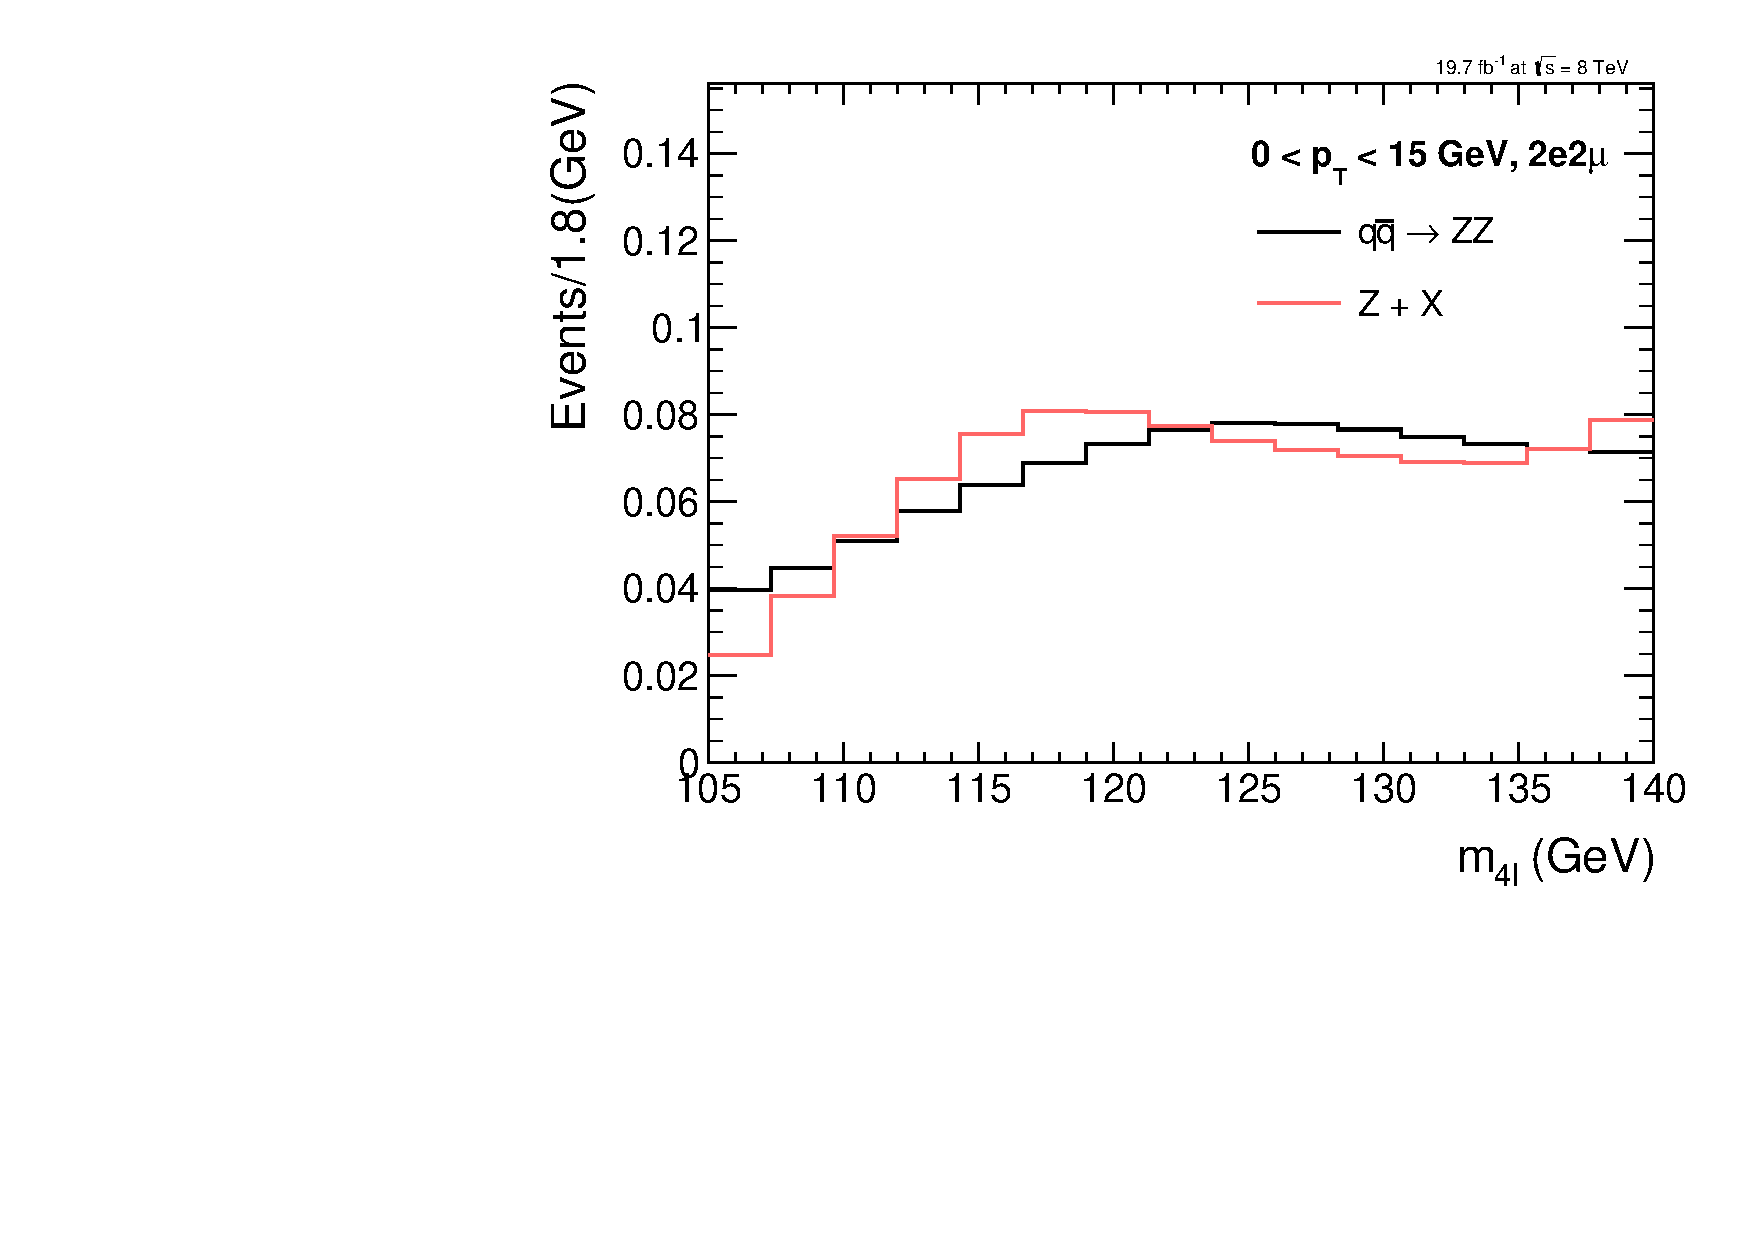
\includegraphics[width=0.30\textwidth,angle=0]{Appendix/figures/XSTemplates_2e2mu_pT4l_0_15_qqZZ_ZJetsCR.pdf}
      \label{fig:bkg-pT4l-qqZZ-ZX-2e2mu:a}
    }    
    \subfigure[$0.0 \GeV < \pt(4\ell) < 15.0 \GeV$]{
      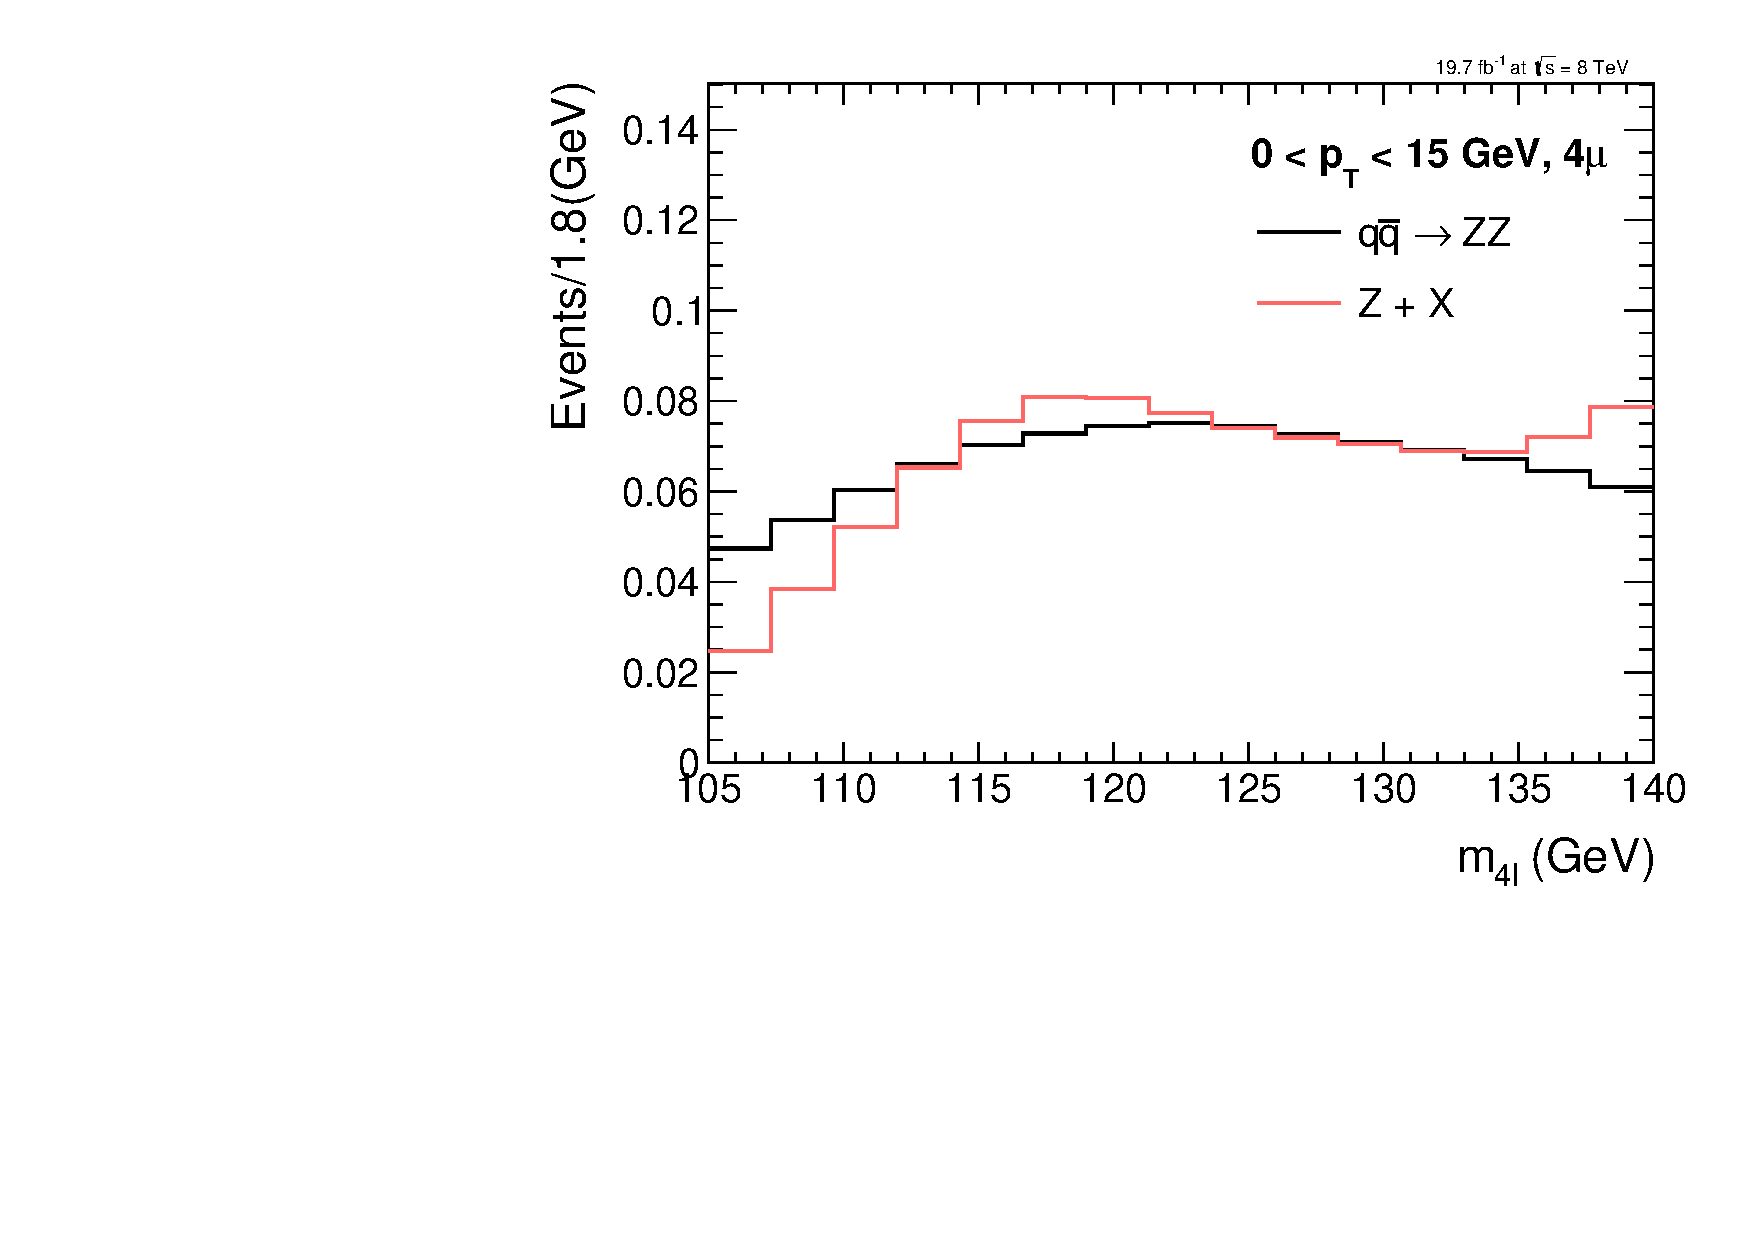
\includegraphics[width=0.30\textwidth,angle=0]{Appendix/figures/XSTemplates_4mu_pT4l_0_15_qqZZ_ZJetsCR.pdf}
      \label{fig:bkg-pT4l-qqZZ-ZX-4mu:a}
    }    
    \subfigure[$0.0 \GeV < \pt(4\ell) < 15.0 \GeV$]{
      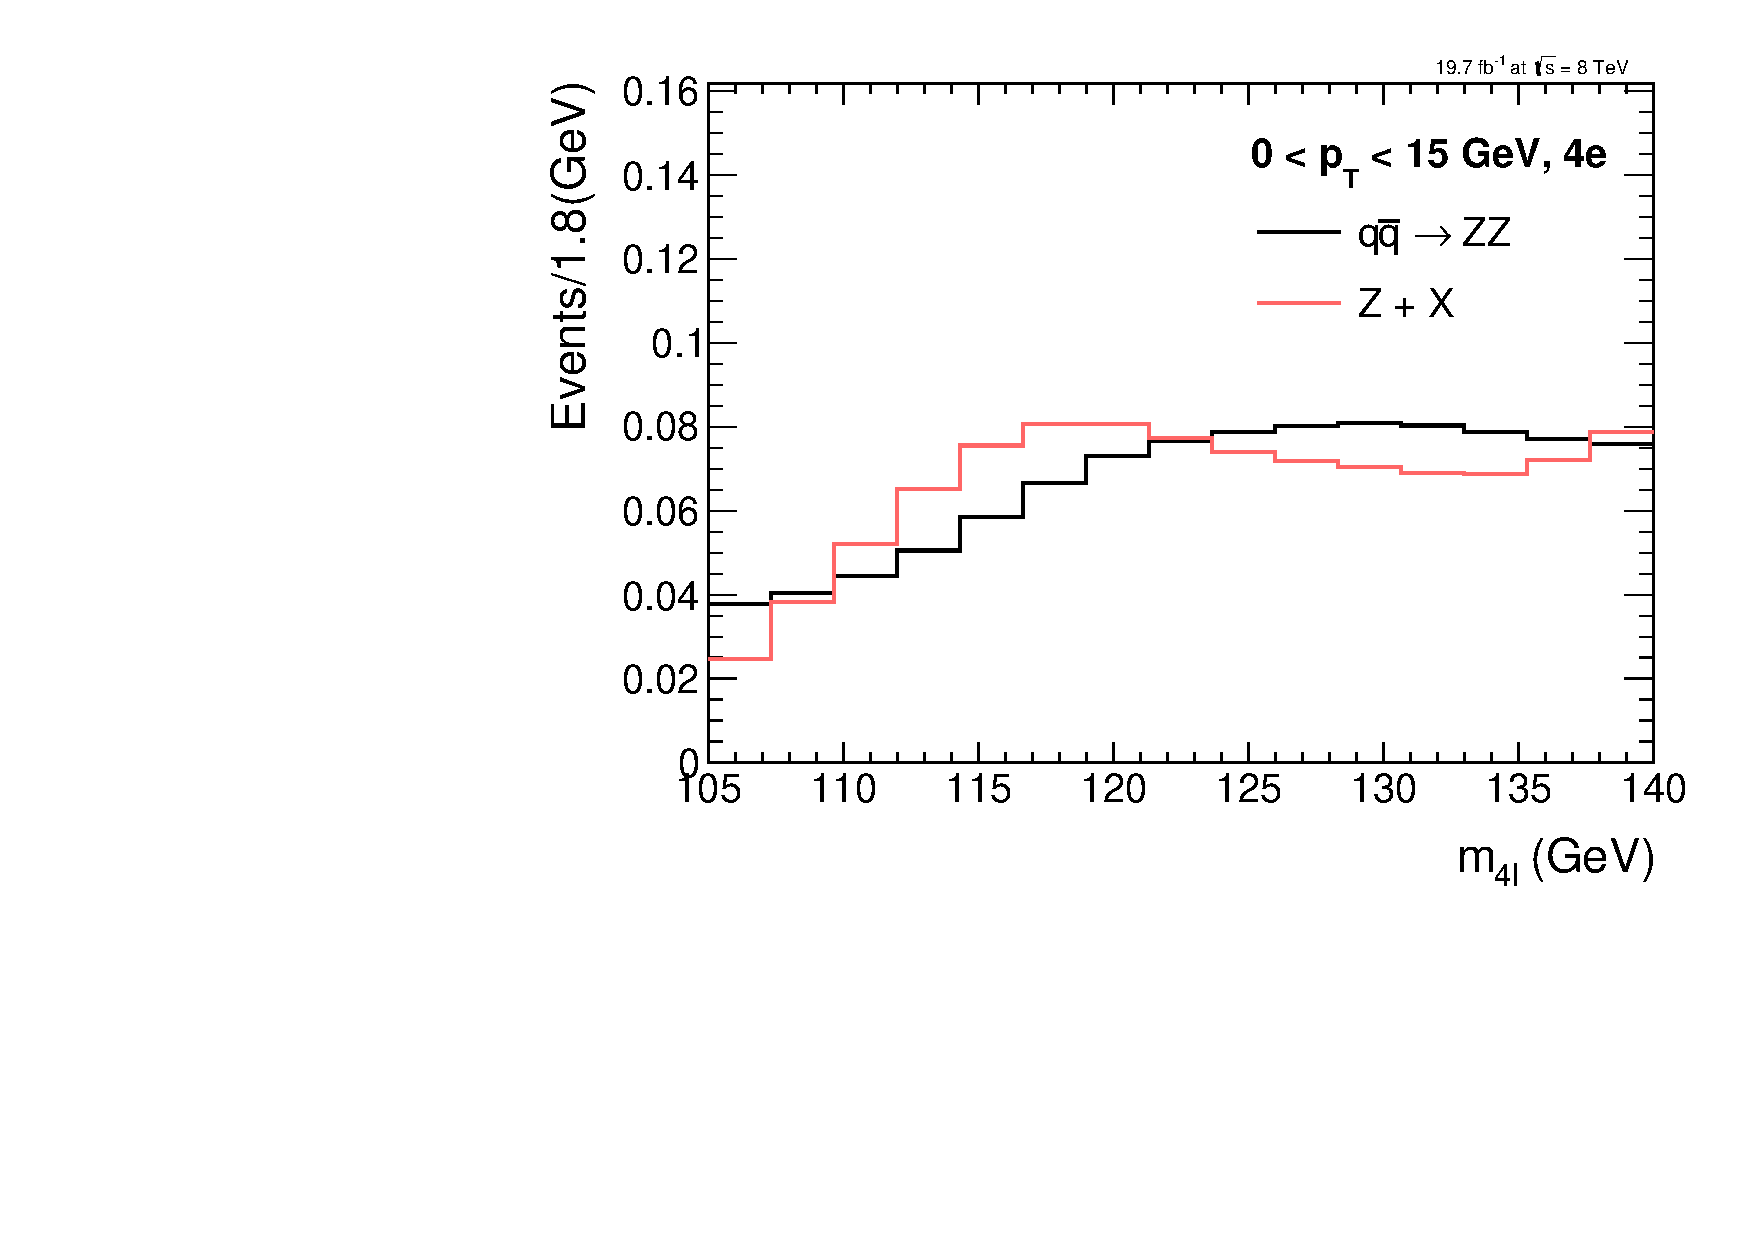
\includegraphics[width=0.30\textwidth,angle=0]{Appendix/figures/XSTemplates_4e_pT4l_0_15_qqZZ_ZJetsCR.pdf}
      \label{fig:bkg-pT4l-qqZZ-ZX-4e:a}
    }    \\

    \subfigure[$15.0 \GeV < \pt(4\ell) < 30.0 \GeV$]{
      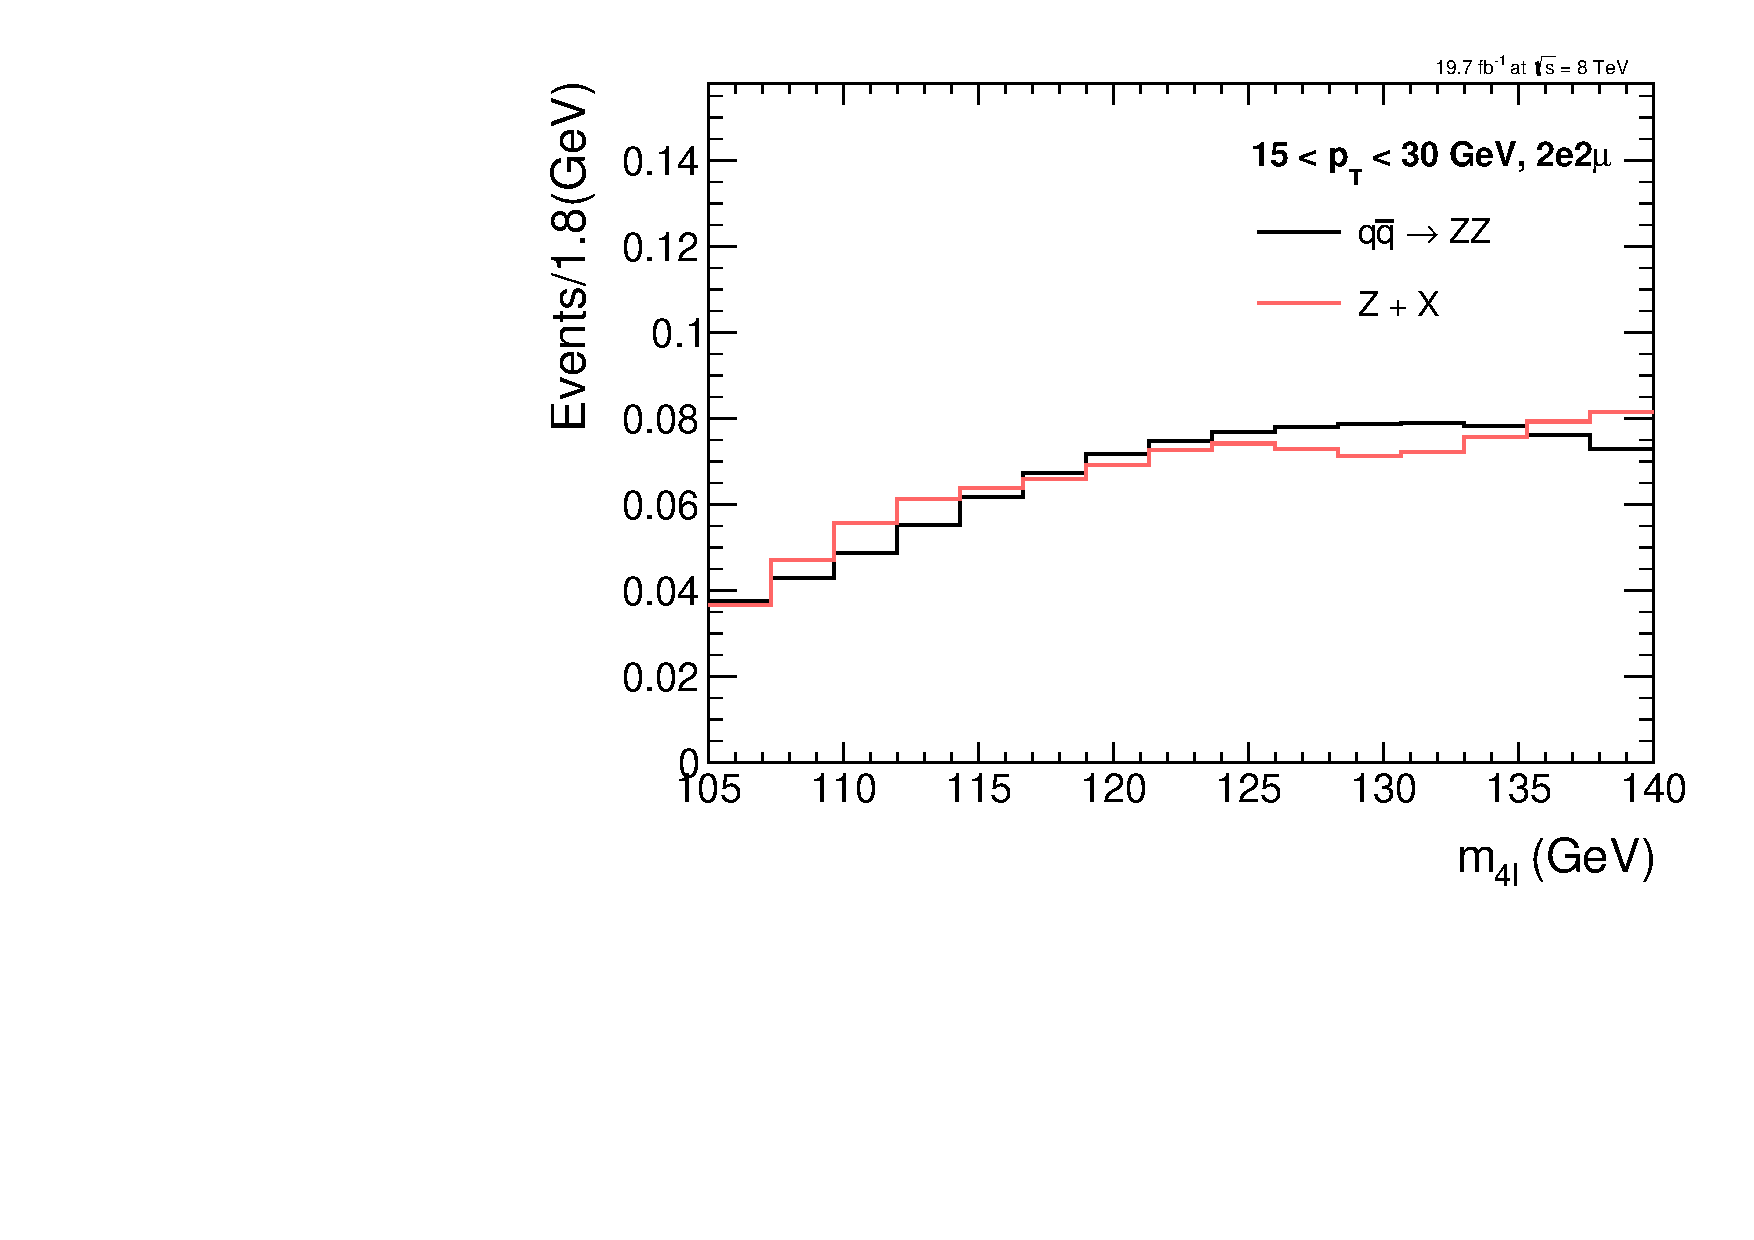
\includegraphics[width=0.30\textwidth,angle=0]{Appendix/figures/XSTemplates_2e2mu_pT4l_15_30_qqZZ_ZJetsCR.pdf}
      \label{fig:bkg-pT4l-qqZZ-ZX-2e2mu:b}
    }
    \subfigure[$15.0 \GeV < \pt(4\ell) < 30.0 \GeV$]{
      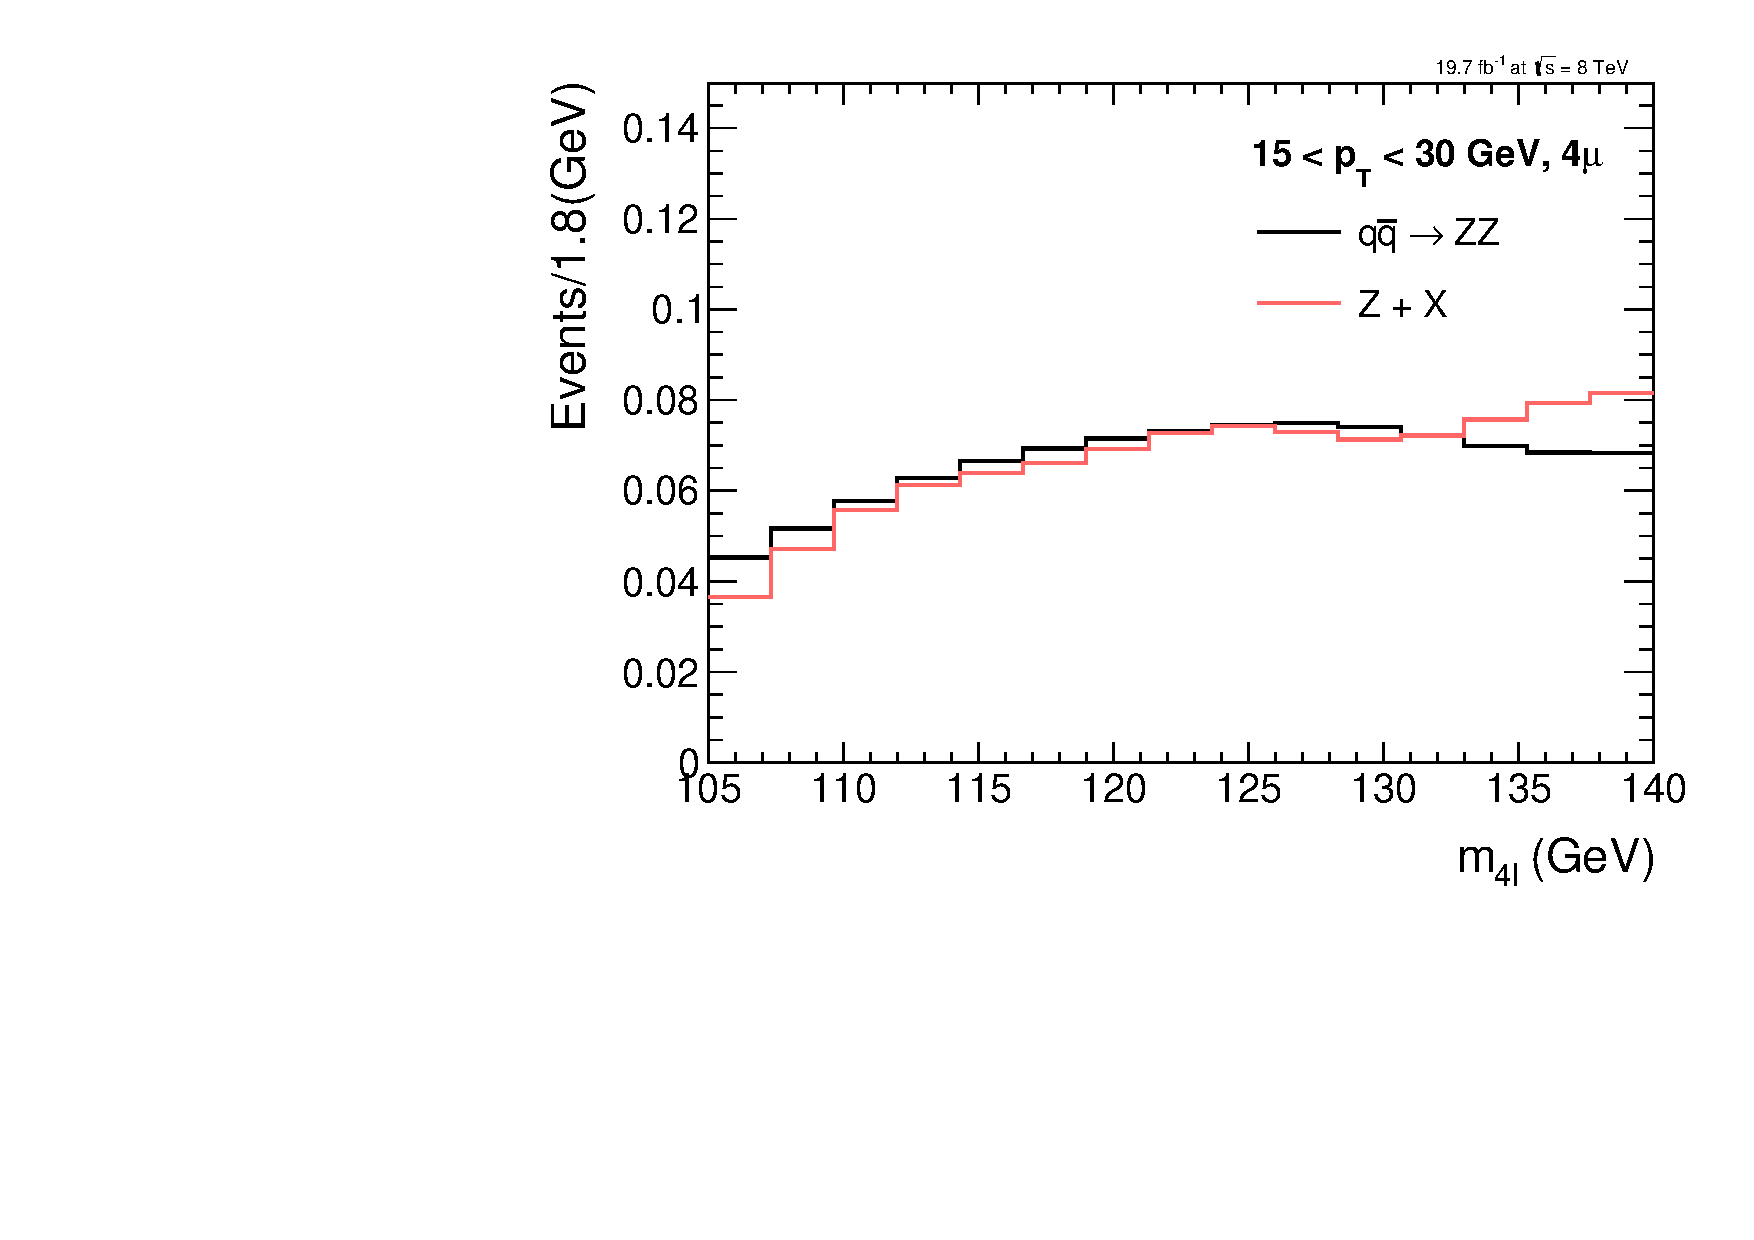
\includegraphics[width=0.30\textwidth,angle=0]{Appendix/figures/XSTemplates_4mu_pT4l_15_30_qqZZ_ZJetsCR.pdf}
      \label{fig:bkg-pT4l-qqZZ-ZX-4mu:b}
    } 
    \subfigure[$15.0 \GeV < \pt(4\ell) < 30.0 \GeV$]{
      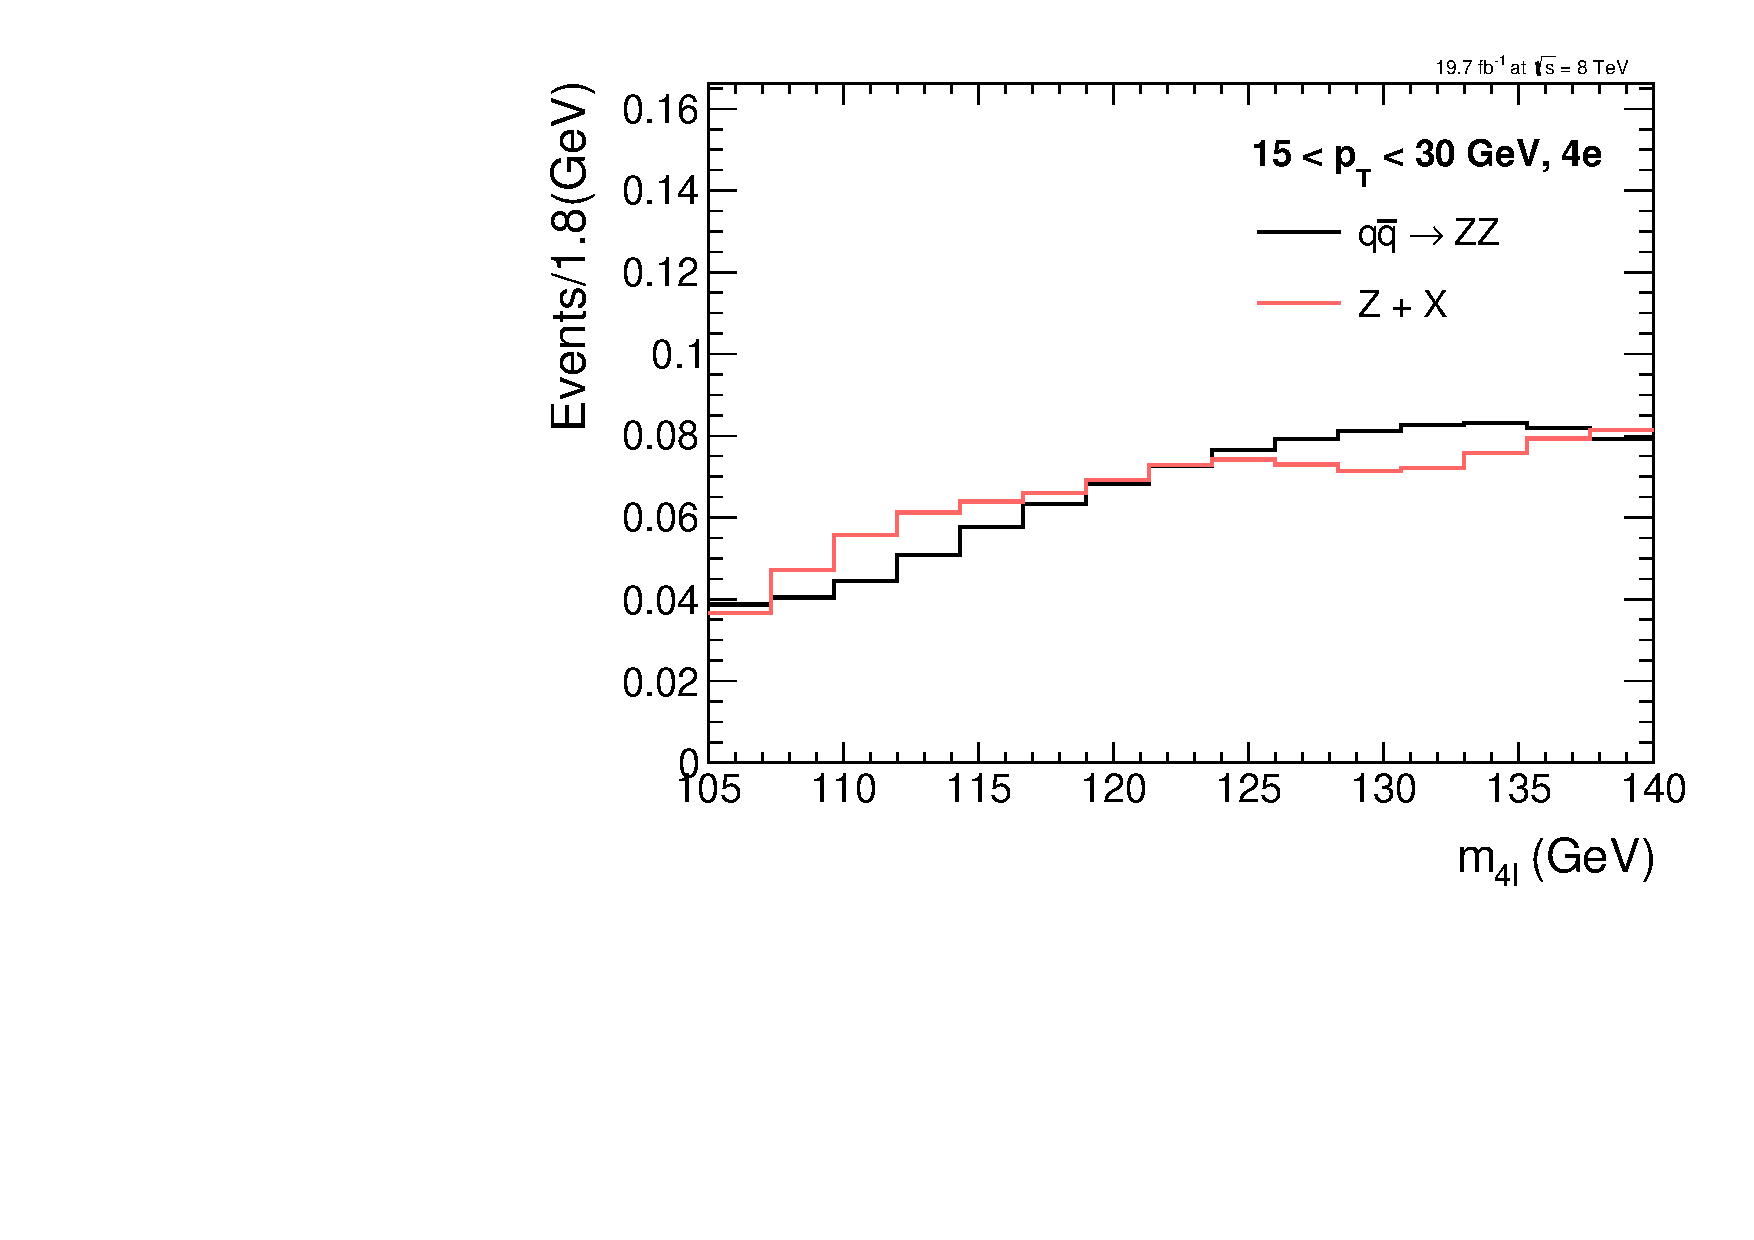
\includegraphics[width=0.30\textwidth,angle=0]{Appendix/figures/XSTemplates_4e_pT4l_15_30_qqZZ_ZJetsCR.pdf}
      \label{fig:bkg-pT4l-qqZZ-ZX-4e:b}
    } \\
    
    \subfigure[$30.0 \GeV < \pt(4\ell) < 60.0 \GeV$]{
      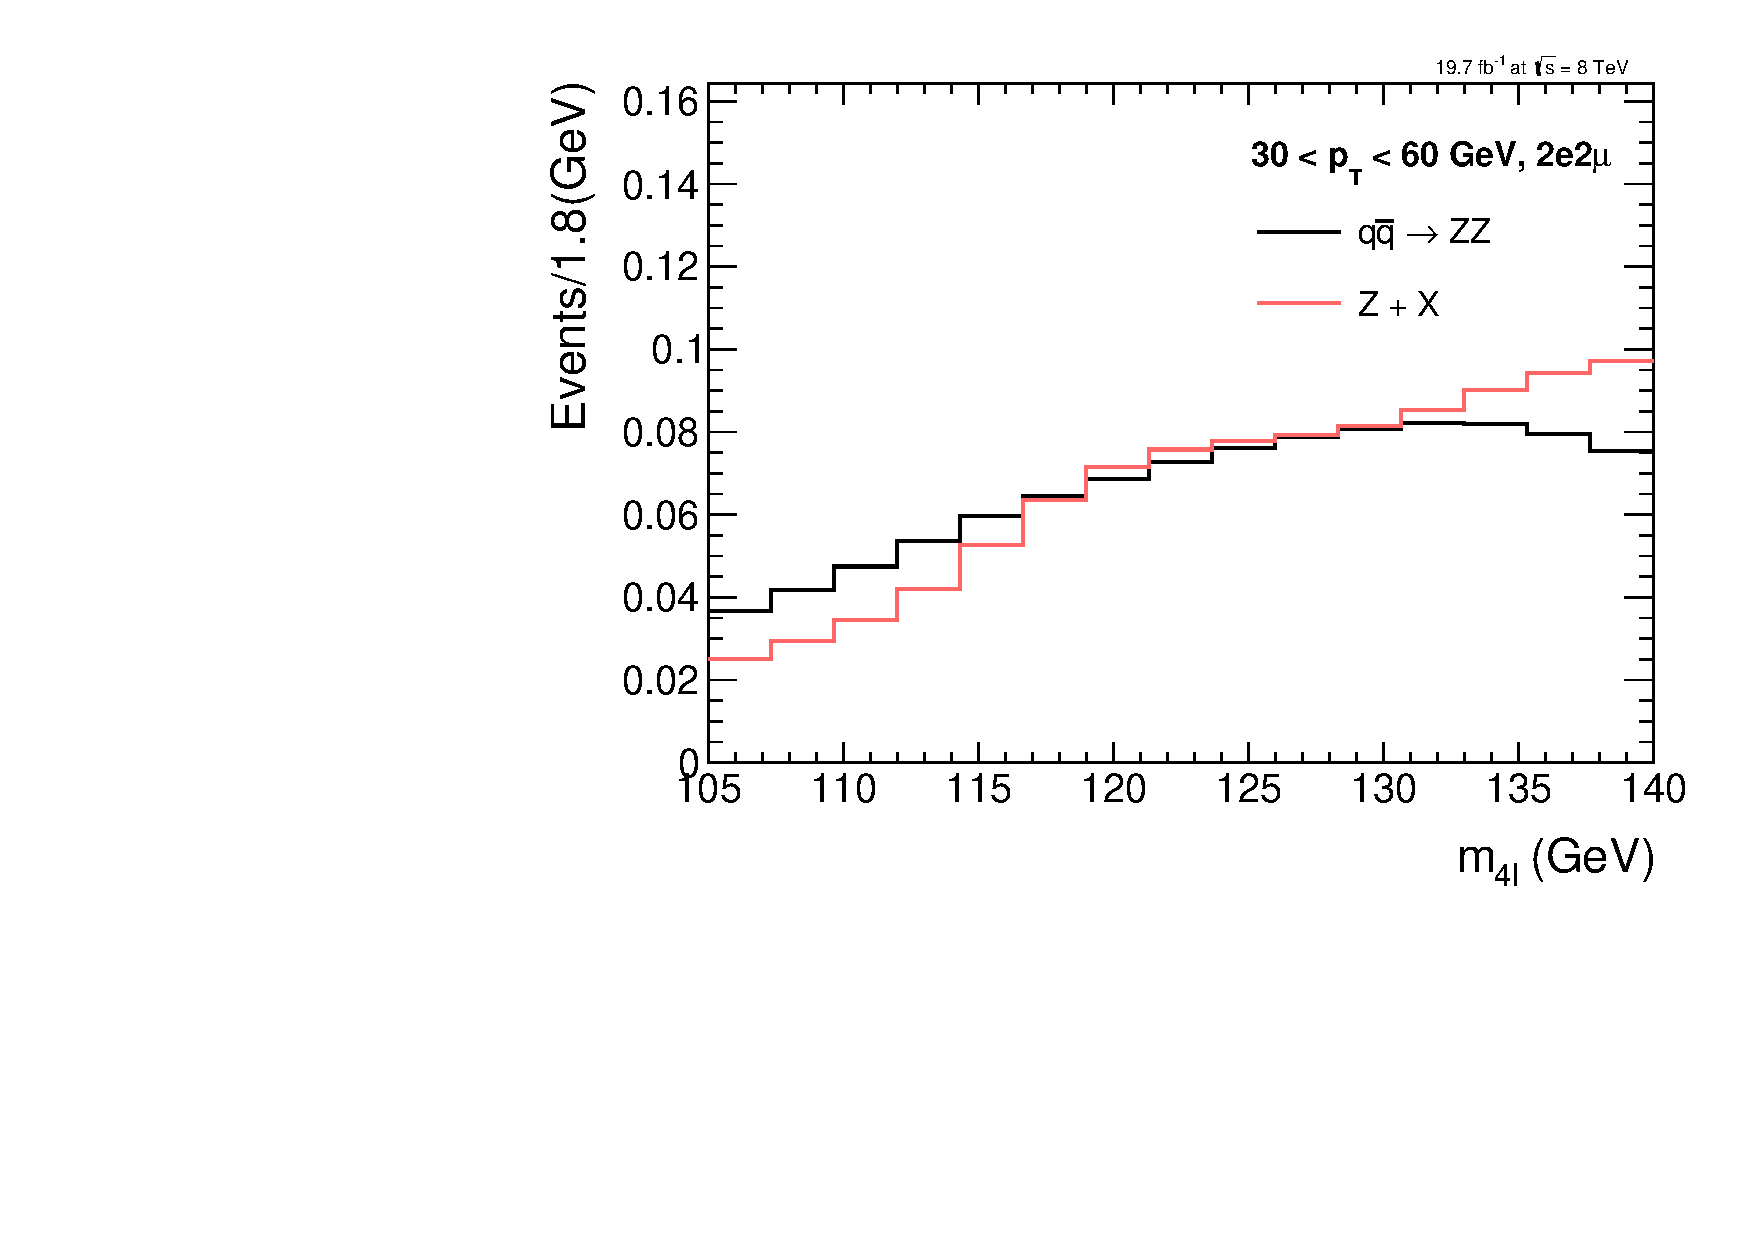
\includegraphics[width=0.30\textwidth,angle=0]{Appendix/figures/XSTemplates_2e2mu_pT4l_30_60_qqZZ_ZJetsCR.pdf}
      \label{fig:bkg-pT4l-qqZZ-ZX-2e2mu:c}
    }
    \subfigure[$30.0 \GeV < \pt(4\ell) < 60.0 \GeV$]{
      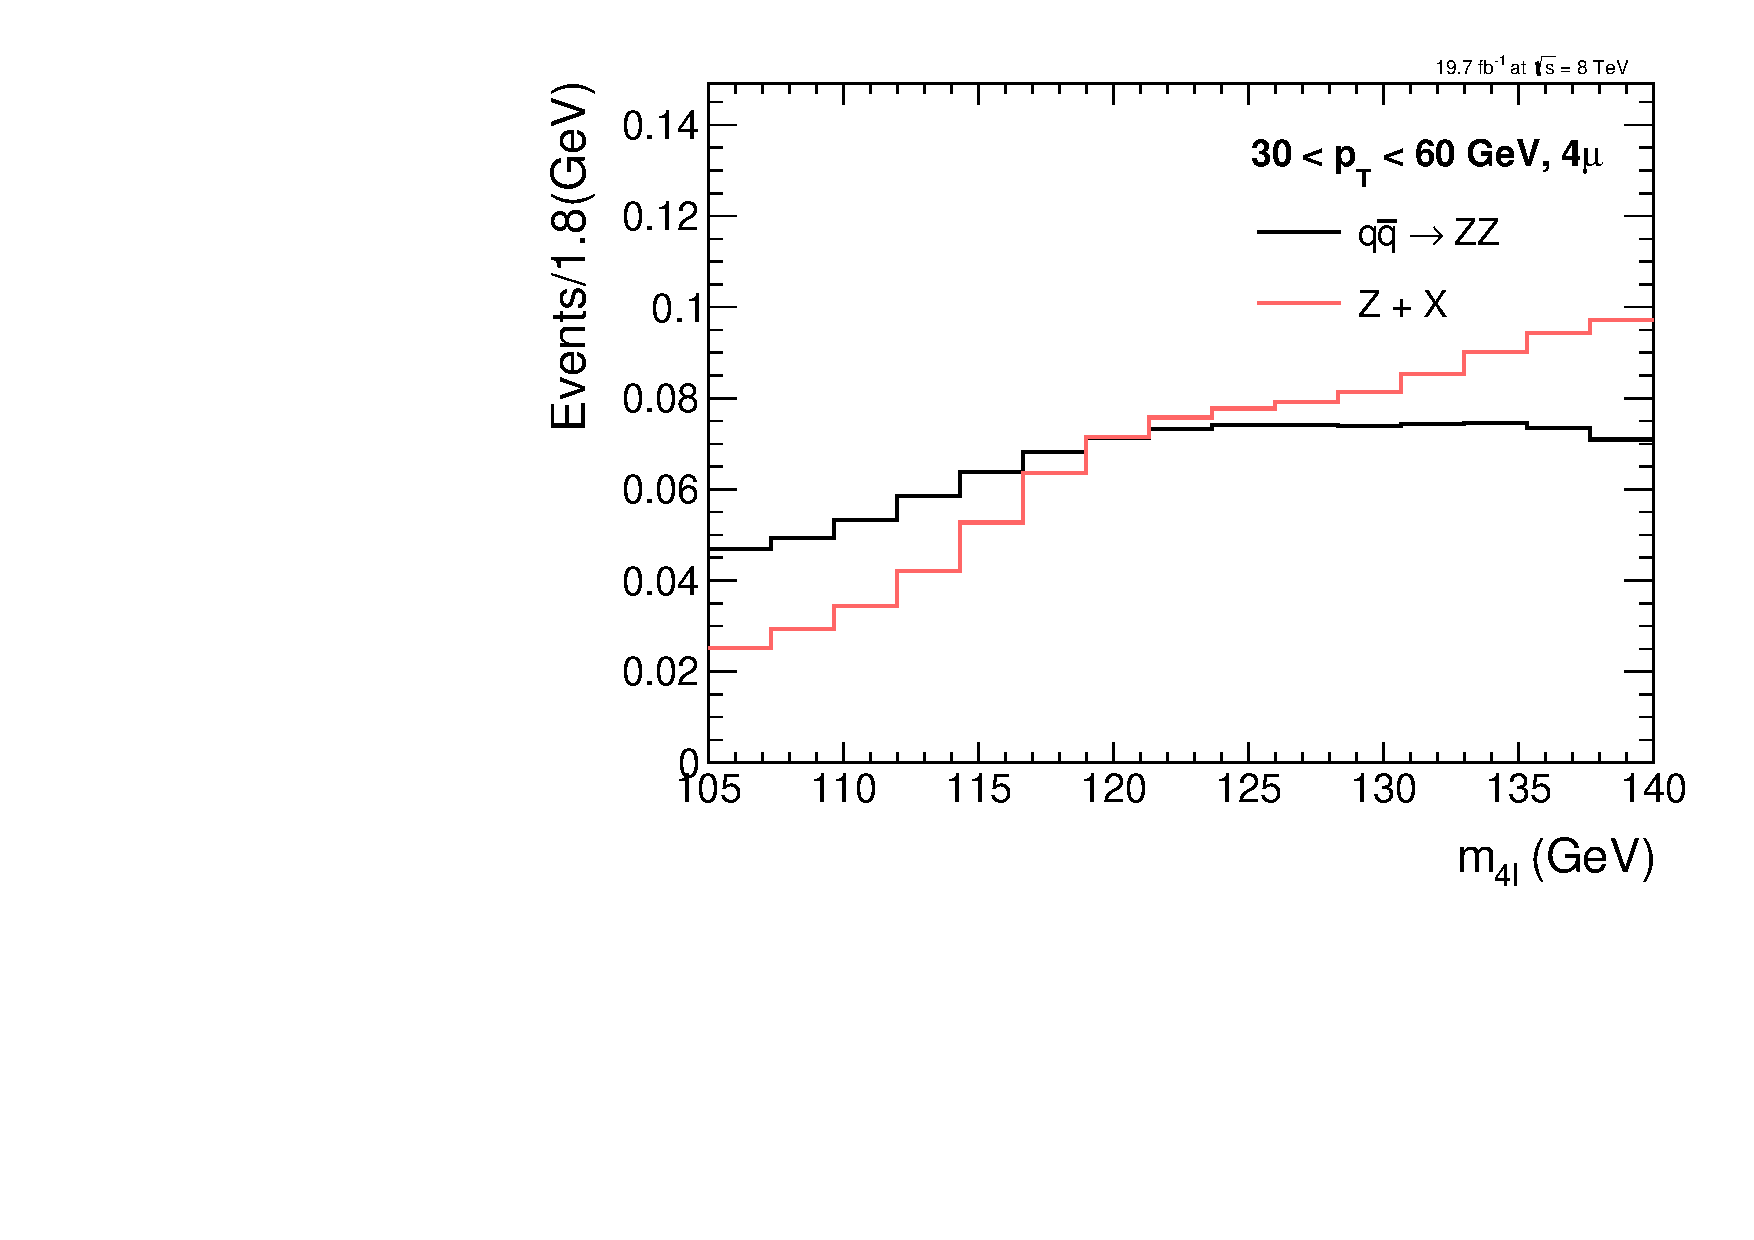
\includegraphics[width=0.30\textwidth,angle=0]{Appendix/figures/XSTemplates_4mu_pT4l_30_60_qqZZ_ZJetsCR.pdf}
      \label{fig:bkg-pT4l-qqZZ-ZX-4mu:c}
    }
    \subfigure[$30.0 \GeV < \pt(4\ell) < 60.0 \GeV$]{
      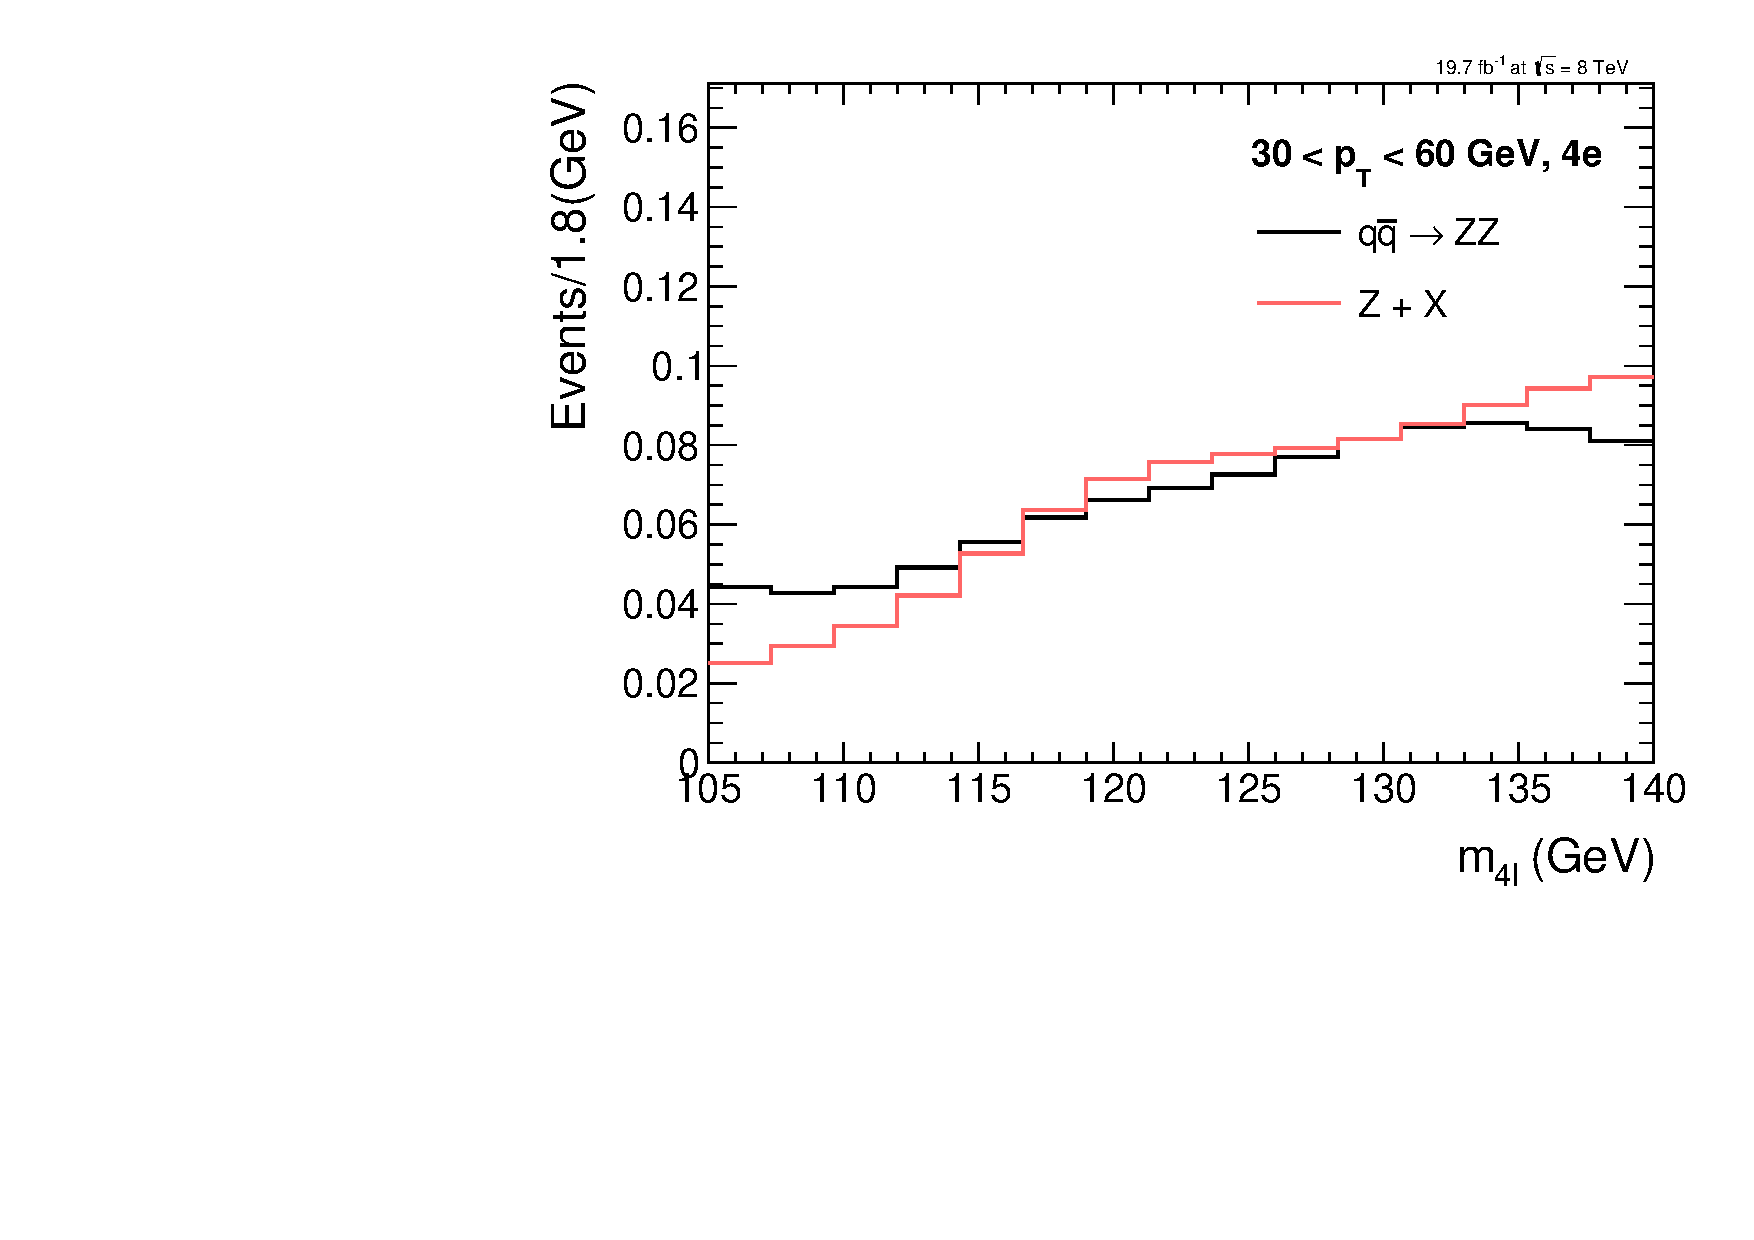
\includegraphics[width=0.30\textwidth,angle=0]{Appendix/figures/XSTemplates_4e_pT4l_30_60_qqZZ_ZJetsCR.pdf}
      \label{fig:bkg-pT4l-qqZZ-ZX-4e:c}
    } \\
    
    \subfigure[$60.0 \GeV < \pt(4\ell) < 1000.0 \GeV$]{
      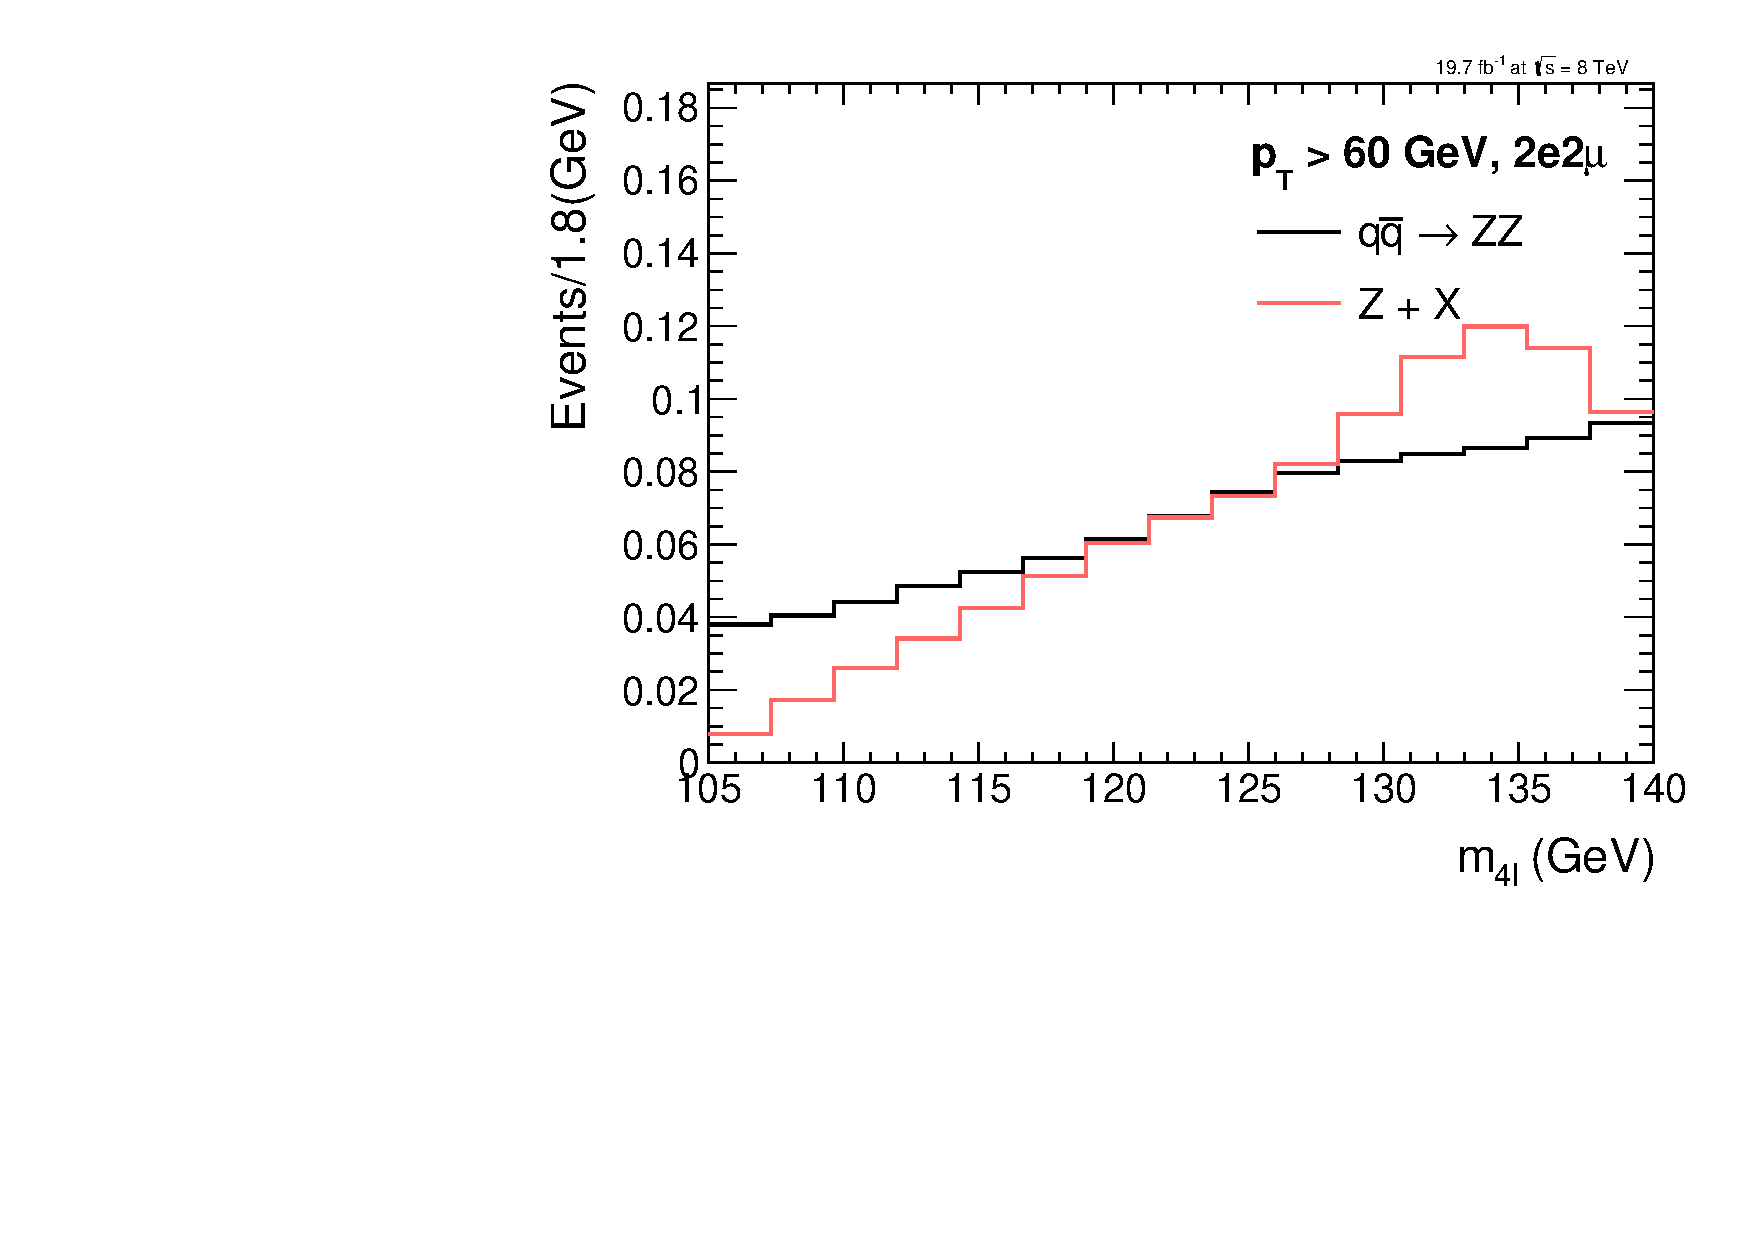
\includegraphics[width=0.30\textwidth,angle=0]{Appendix/figures/XSTemplates_2e2mu_pT4l_60_200_qqZZ_ZJetsCR.pdf}
      \label{fig:bkg-pT4l-qqZZ-ZX-2e2mu:d}
    }
    \subfigure[$60.0 \GeV < \pt(4\ell) < 1000.0 \GeV$]{
      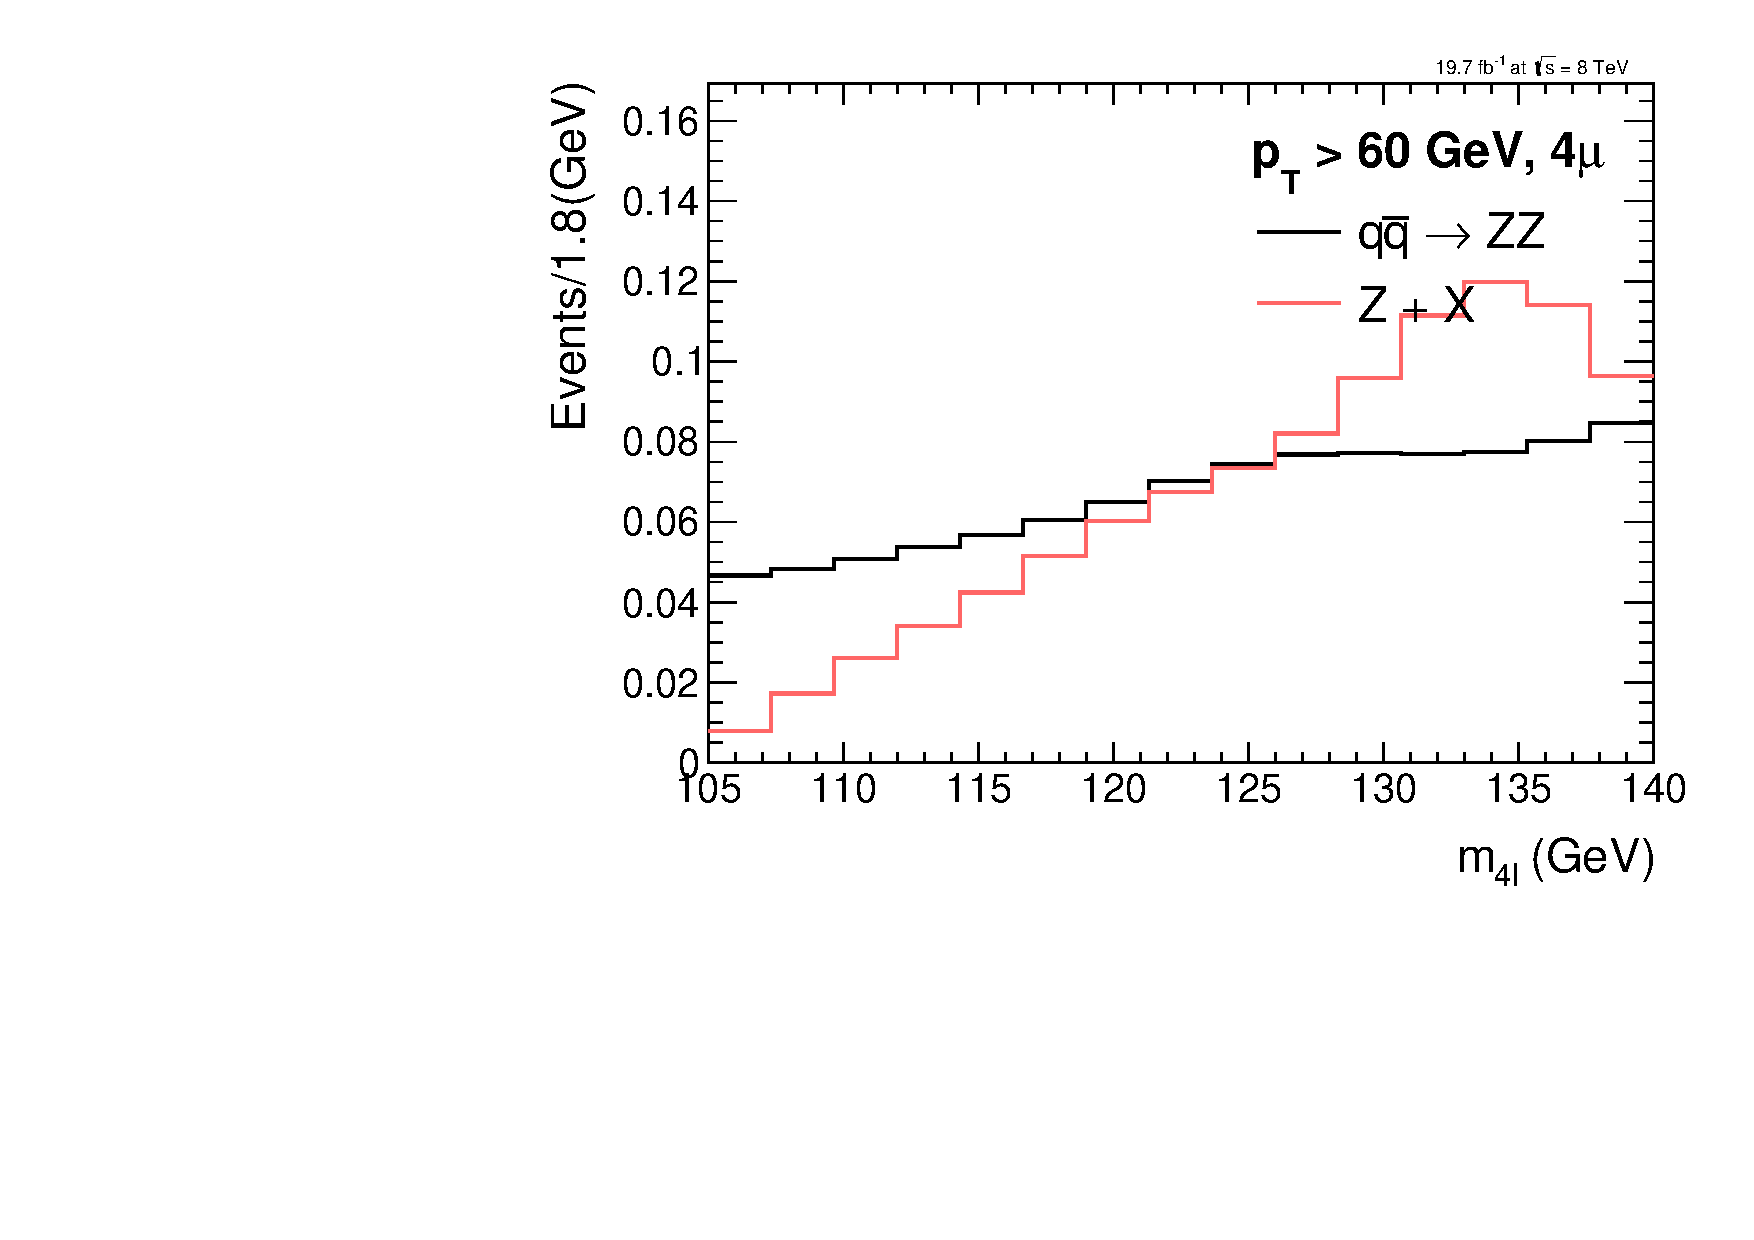
\includegraphics[width=0.30\textwidth,angle=0]{Appendix/figures/XSTemplates_4mu_pT4l_60_200_qqZZ_ZJetsCR.pdf}
      \label{fig:bkg-pT4l-qqZZ-ZX-4mu:d}
    }
    \subfigure[$60.0 \GeV < \pt(4\ell) < 1000.0 \GeV$]{
      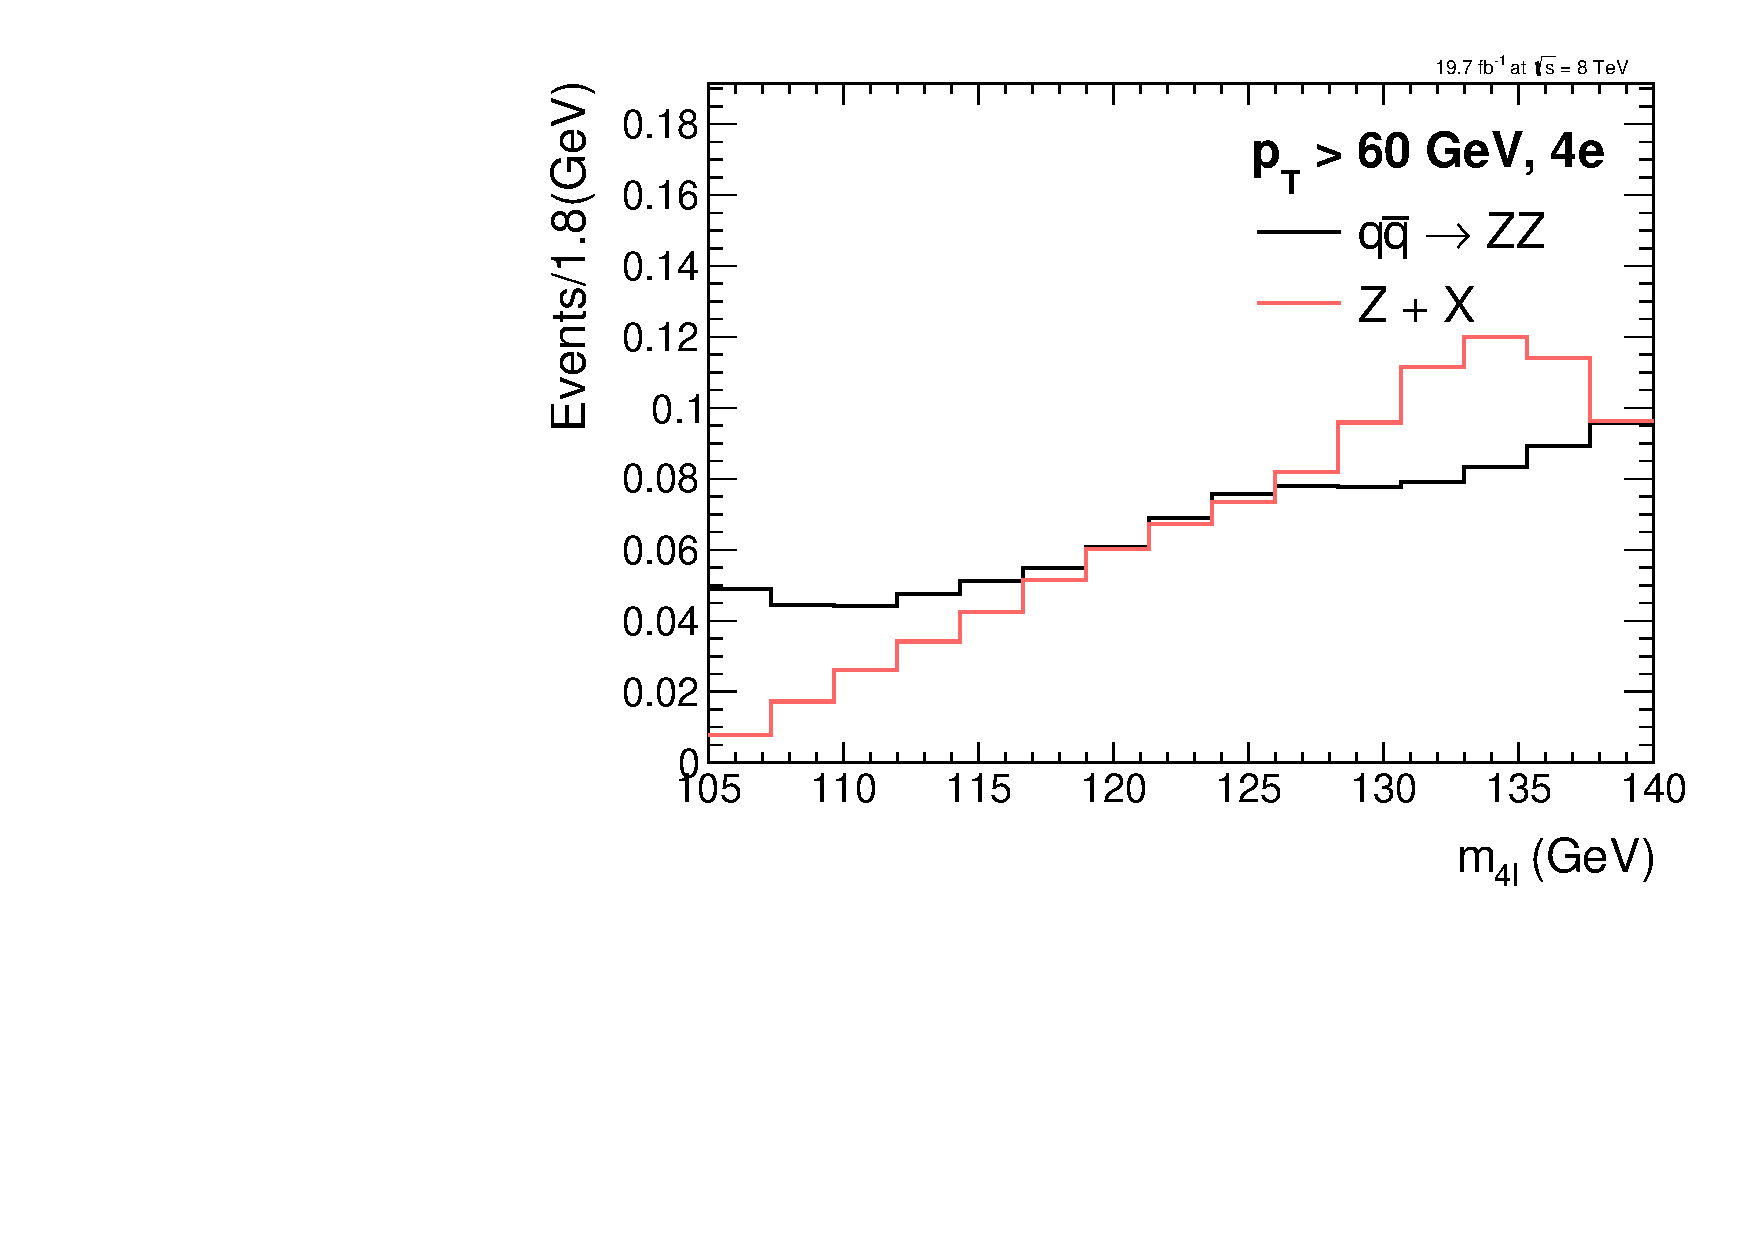
\includegraphics[width=0.30\textwidth,angle=0]{Appendix/figures/XSTemplates_4e_pT4l_60_200_qqZZ_ZJetsCR.pdf}
      \label{fig:bkg-pT4l-qqZZ-ZX-4e:d}
    } \\
    
    \caption{ Distributions of m($4\ell$) for the $qq \rightarrow \mathrm{ZZ}$ and Z+X backgrounds in different bins of $\pt(4\ell)$ 
    for three final states: $2e2\mu$(left), $4\mu$(middle) and $4e$(right).}
  \label{fig:bkg-pT4l-qqZZ-ZX}
  
 \end{center}
\end{figure} 

 \clearpage
 
 \begin{figure}[!ht]
  \begin{center}
  
    \subfigure[$0.0 \GeV < \pt(4\ell) < 15.0 \GeV$]{
      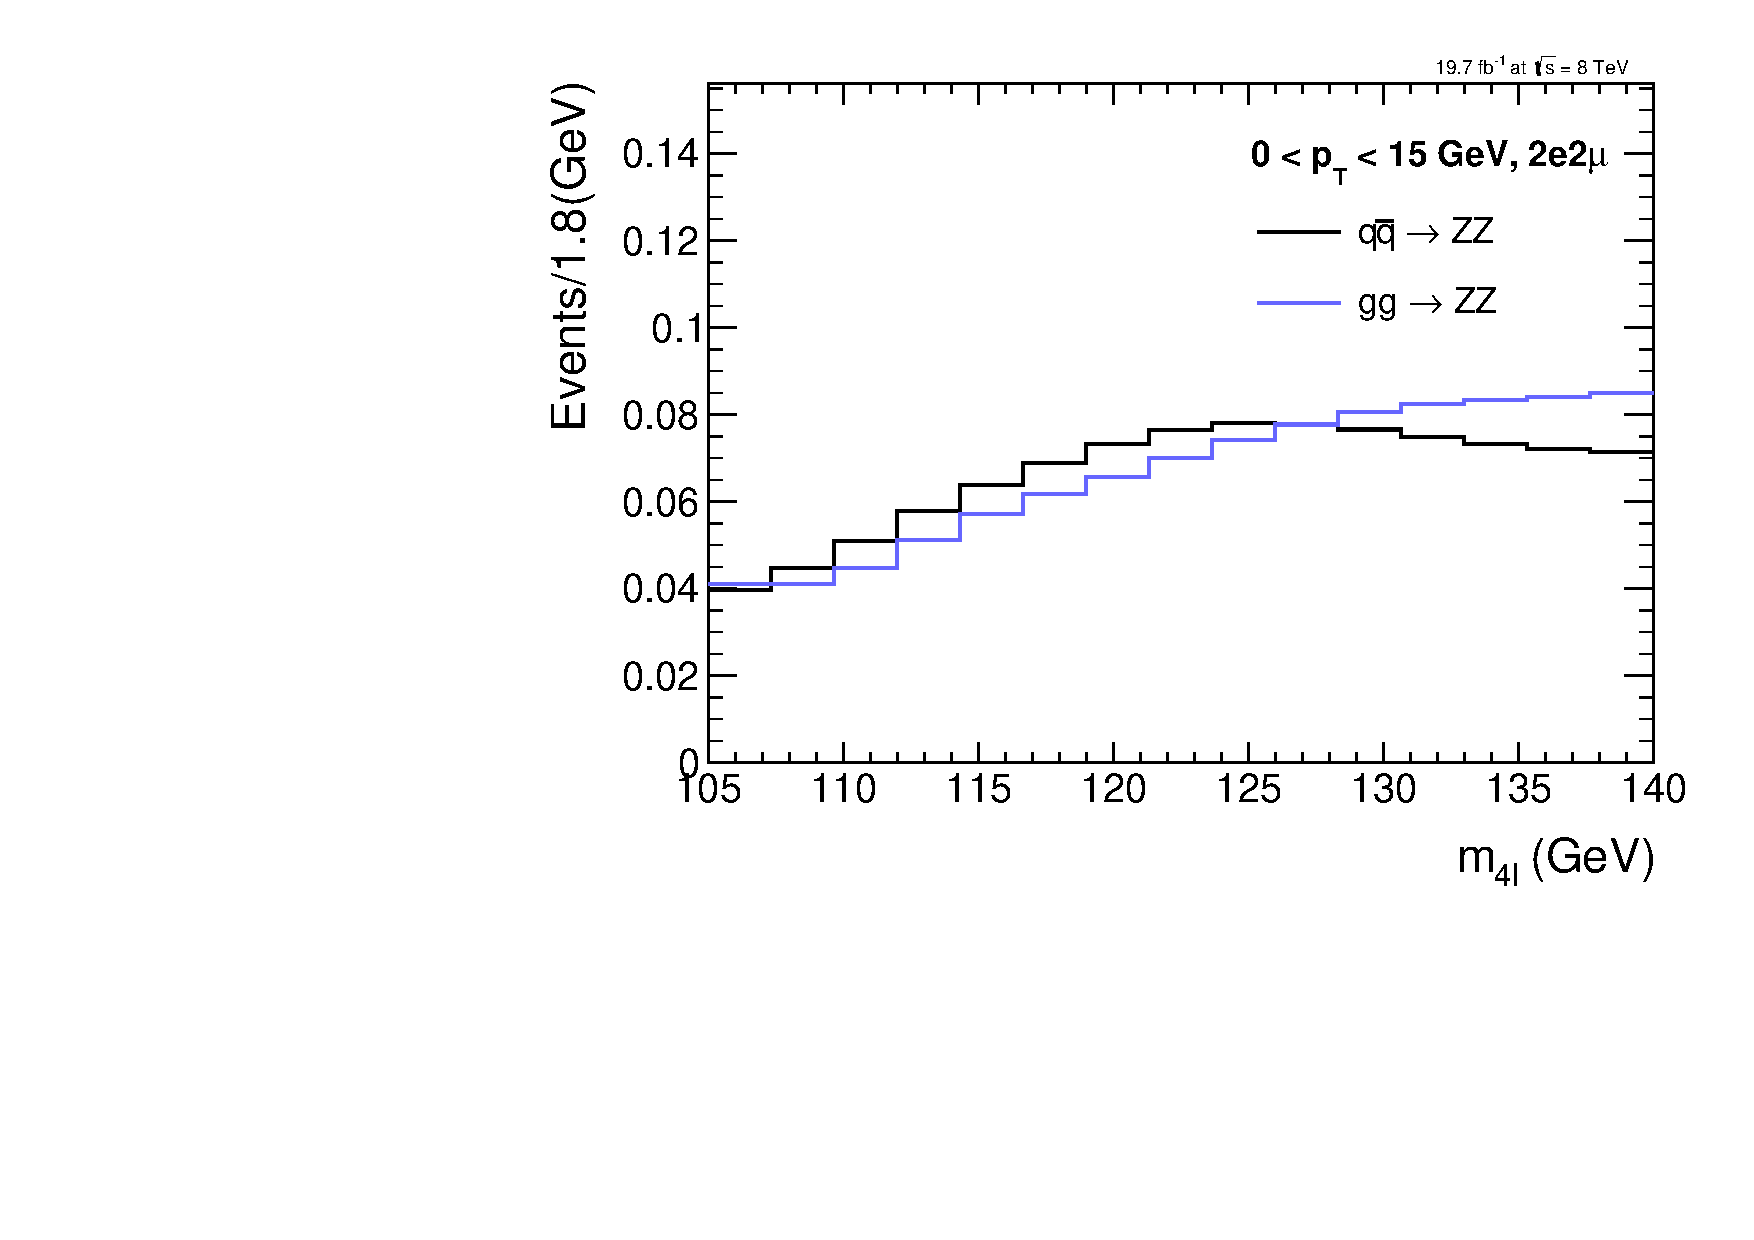
\includegraphics[width=0.30\textwidth,angle=0]{Appendix/figures/XSTemplates_2e2mu_pT4l_0_15_qqZZ_ggZZ.pdf}
      \label{fig:bkg-pT4l-qqZZ-ggZZ-2e2mu:a}
    }    
    \subfigure[$0.0 \GeV < \pt(4\ell) < 15.0 \GeV$]{
      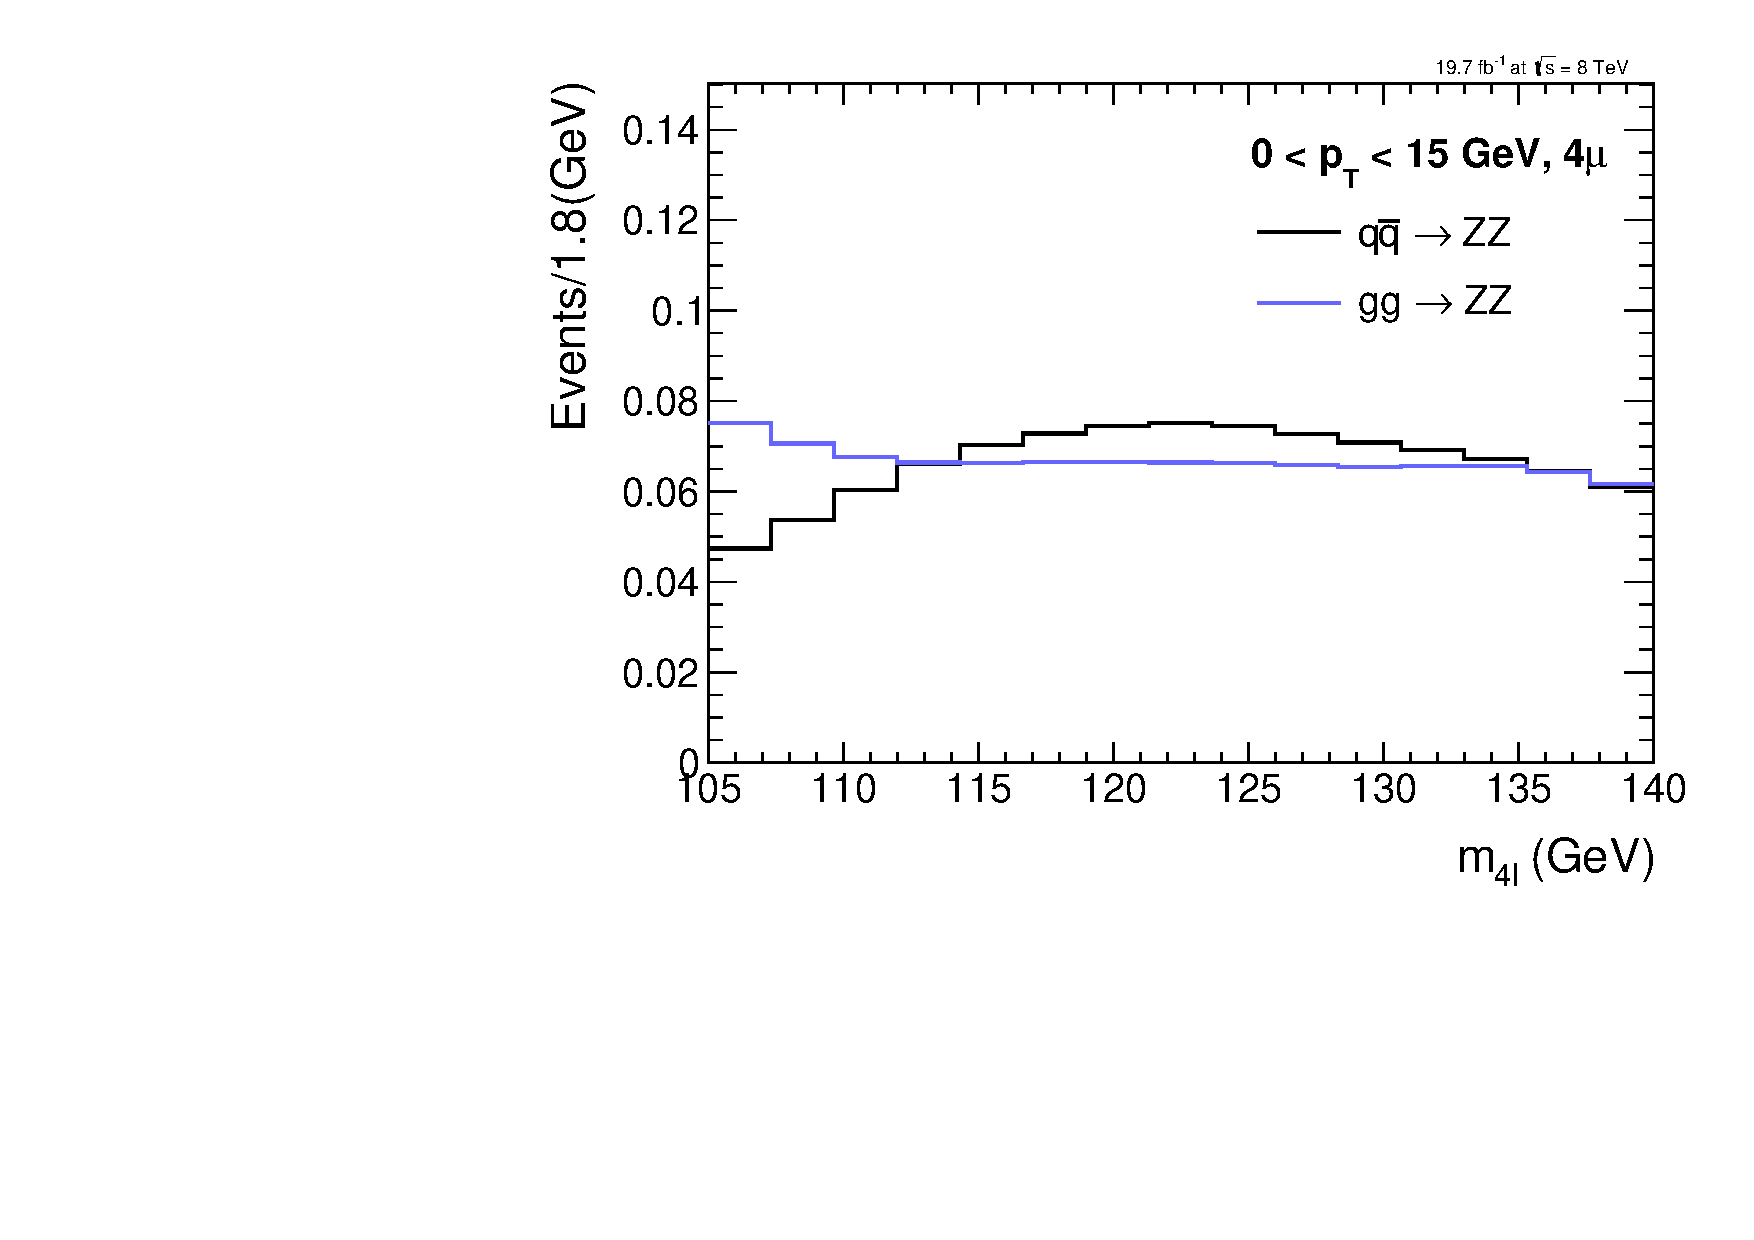
\includegraphics[width=0.30\textwidth,angle=0]{Appendix/figures/XSTemplates_4mu_pT4l_0_15_qqZZ_ggZZ.pdf}
      \label{fig:bkg-pT4l-qqZZ-ggZZ-4mu:a}
    }    
    \subfigure[$0.0 \GeV < \pt(4\ell) < 15.0 \GeV$]{
      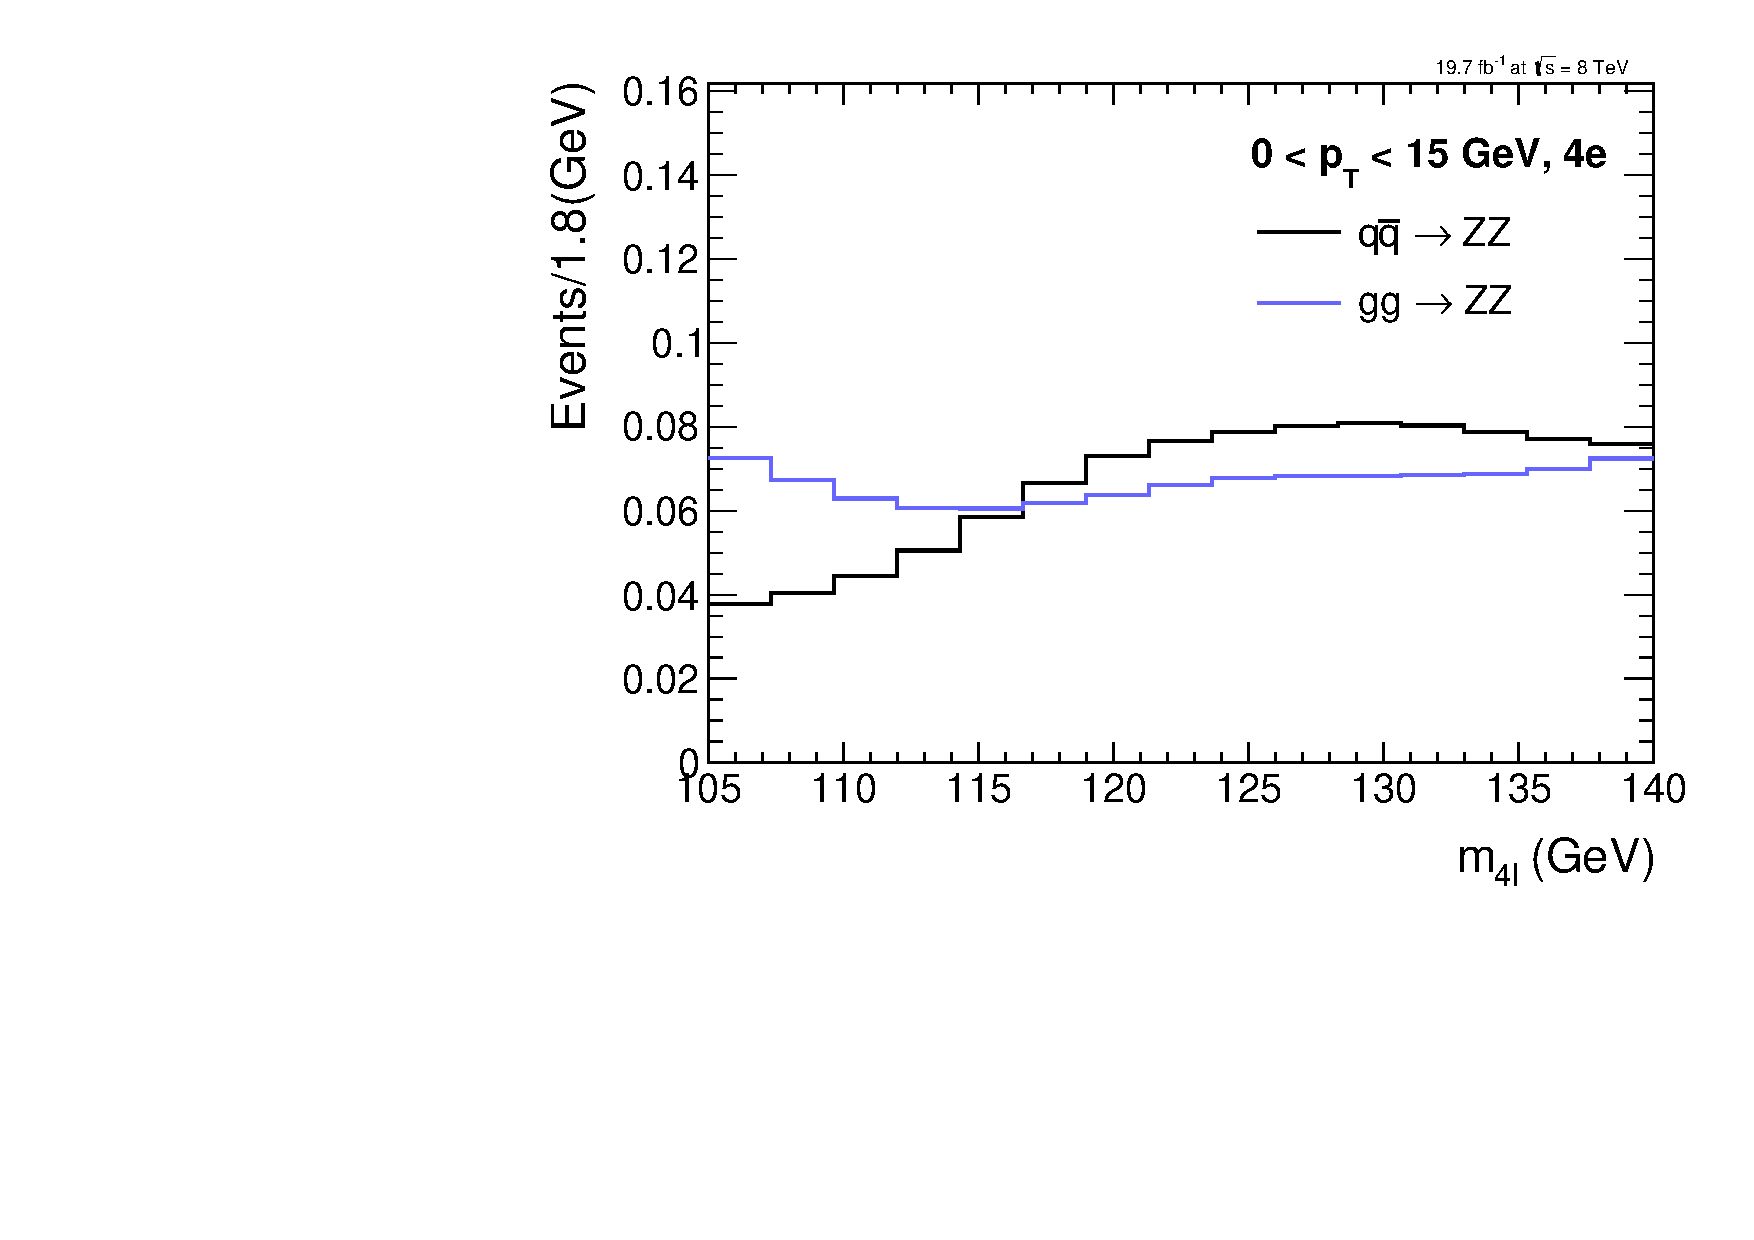
\includegraphics[width=0.30\textwidth,angle=0]{Appendix/figures/XSTemplates_4e_pT4l_0_15_qqZZ_ggZZ.pdf}
      \label{fig:bkg-pT4l-qqZZ-ggZZ-4e:a}
    }    \\

    \subfigure[$15.0 \GeV < \pt(4\ell) < 30.0 \GeV$]{
      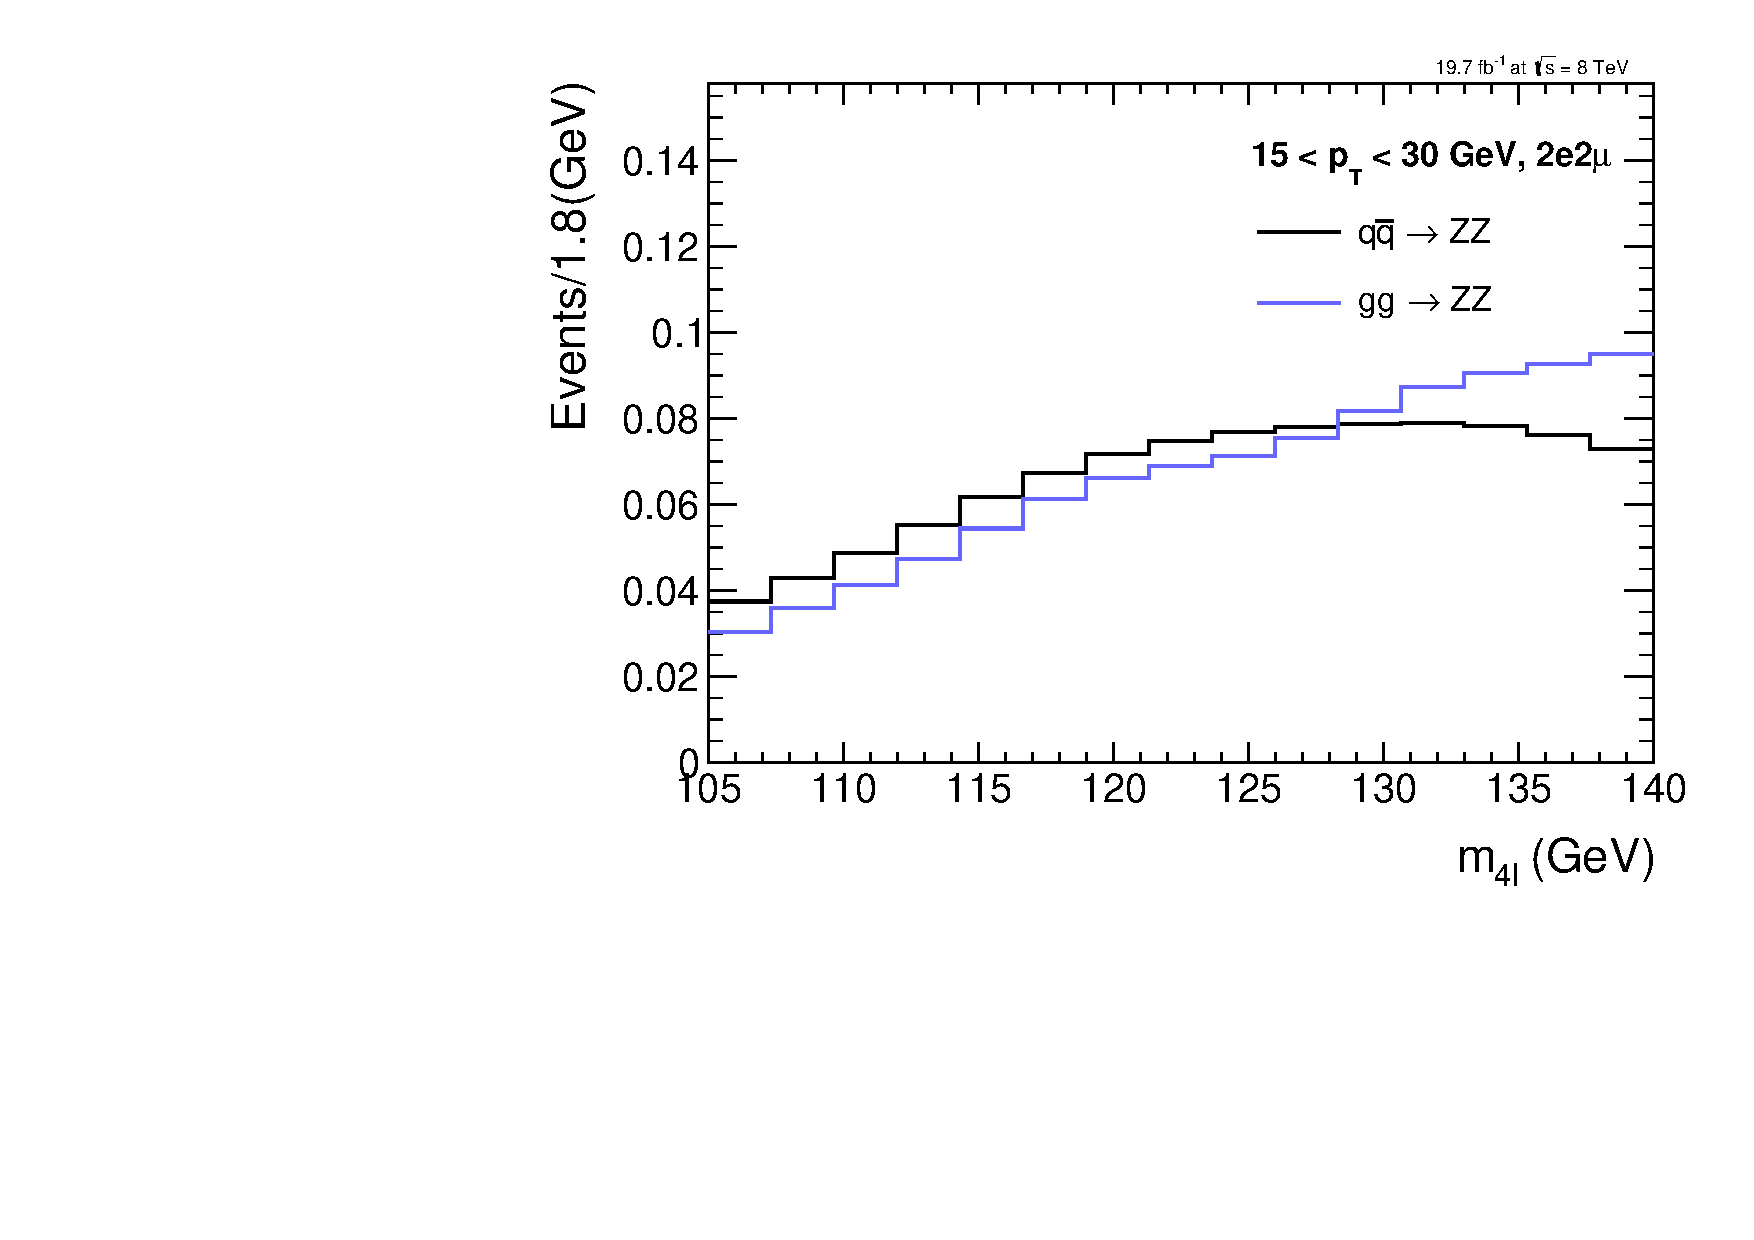
\includegraphics[width=0.30\textwidth,angle=0]{Appendix/figures/XSTemplates_2e2mu_pT4l_15_30_qqZZ_ggZZ.pdf}
      \label{fig:bkg-pT4l-qqZZ-ggZZ-2e2mu:b}
    }
    \subfigure[$15.0 \GeV < \pt(4\ell) < 30.0 \GeV$]{
      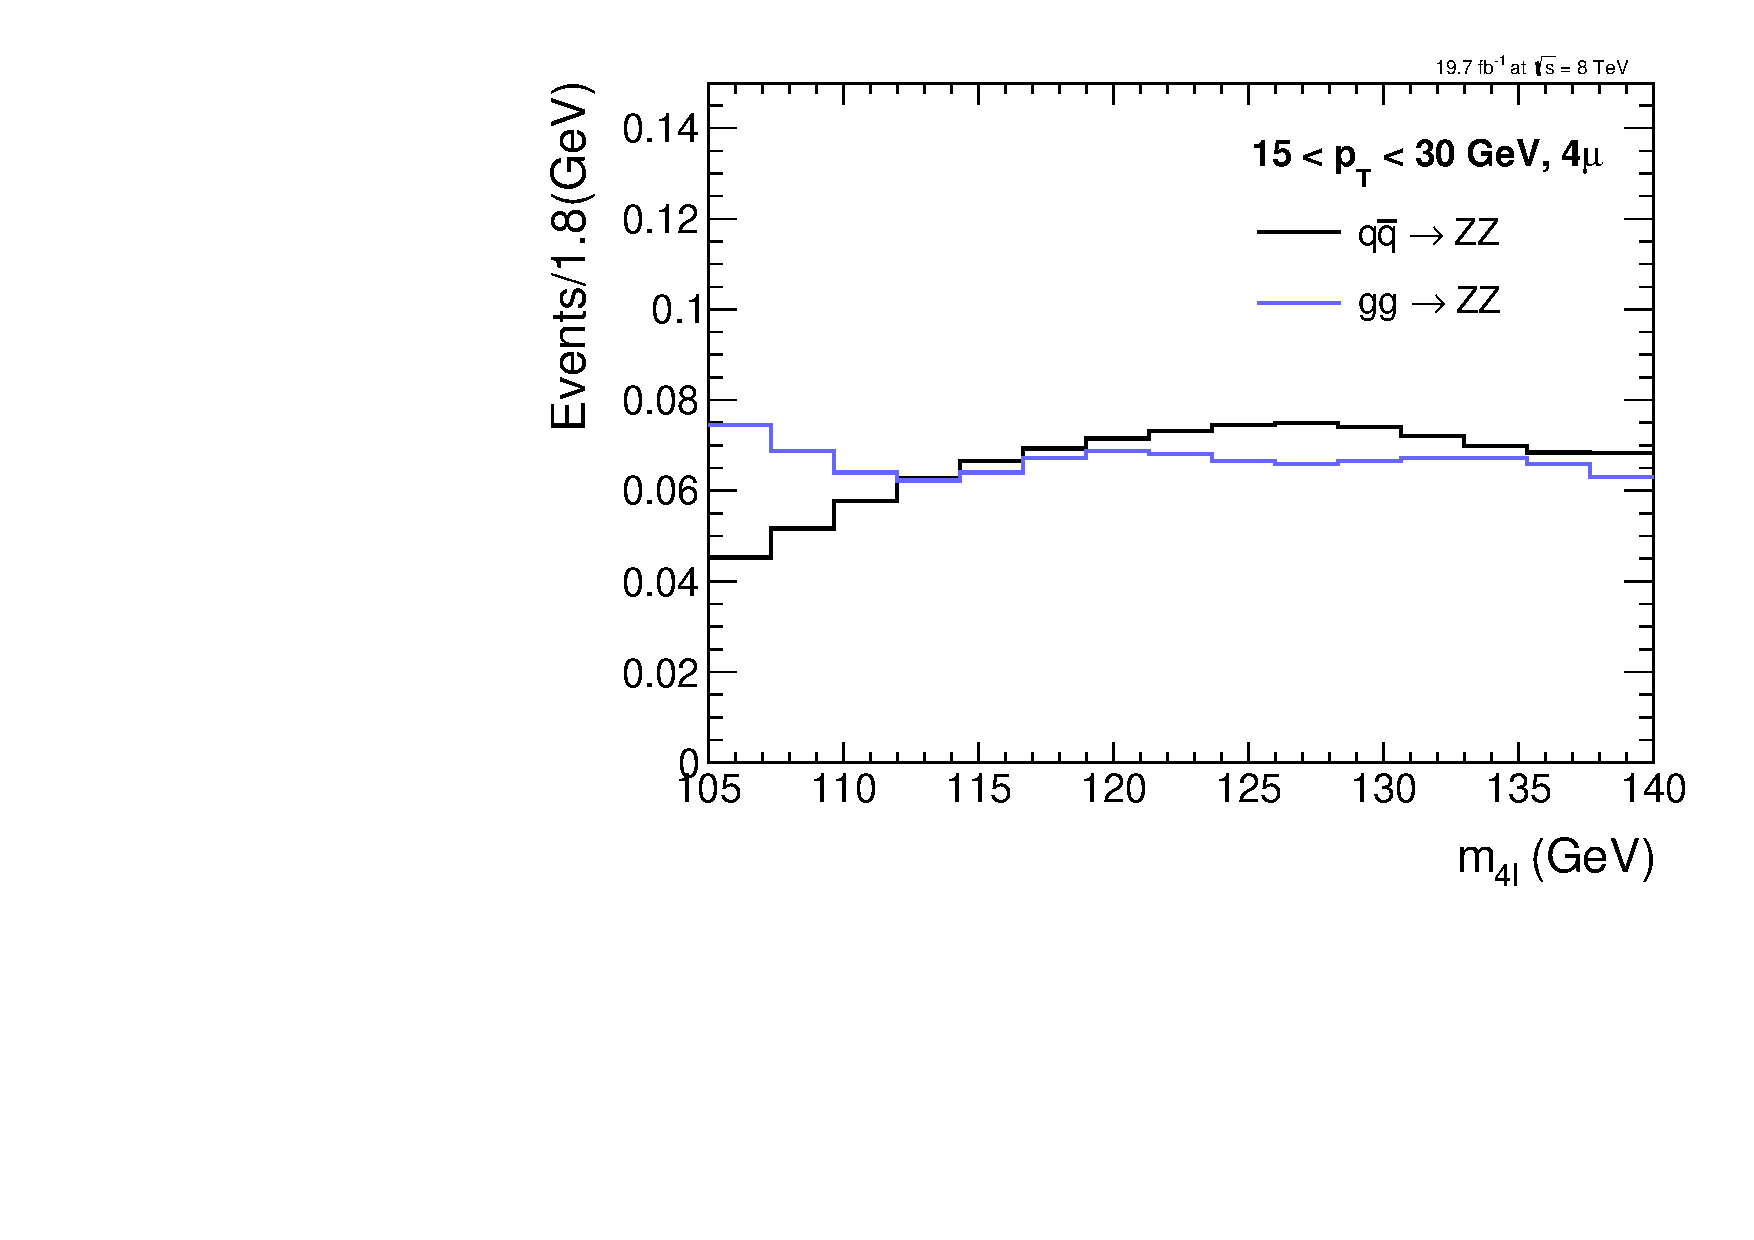
\includegraphics[width=0.30\textwidth,angle=0]{Appendix/figures/XSTemplates_4mu_pT4l_15_30_qqZZ_ggZZ.pdf}
      \label{fig:bkg-pT4l-qqZZ-ggZZ-4mu:b}
    } 
    \subfigure[$15.0 \GeV < \pt(4\ell) < 30.0 \GeV$]{
      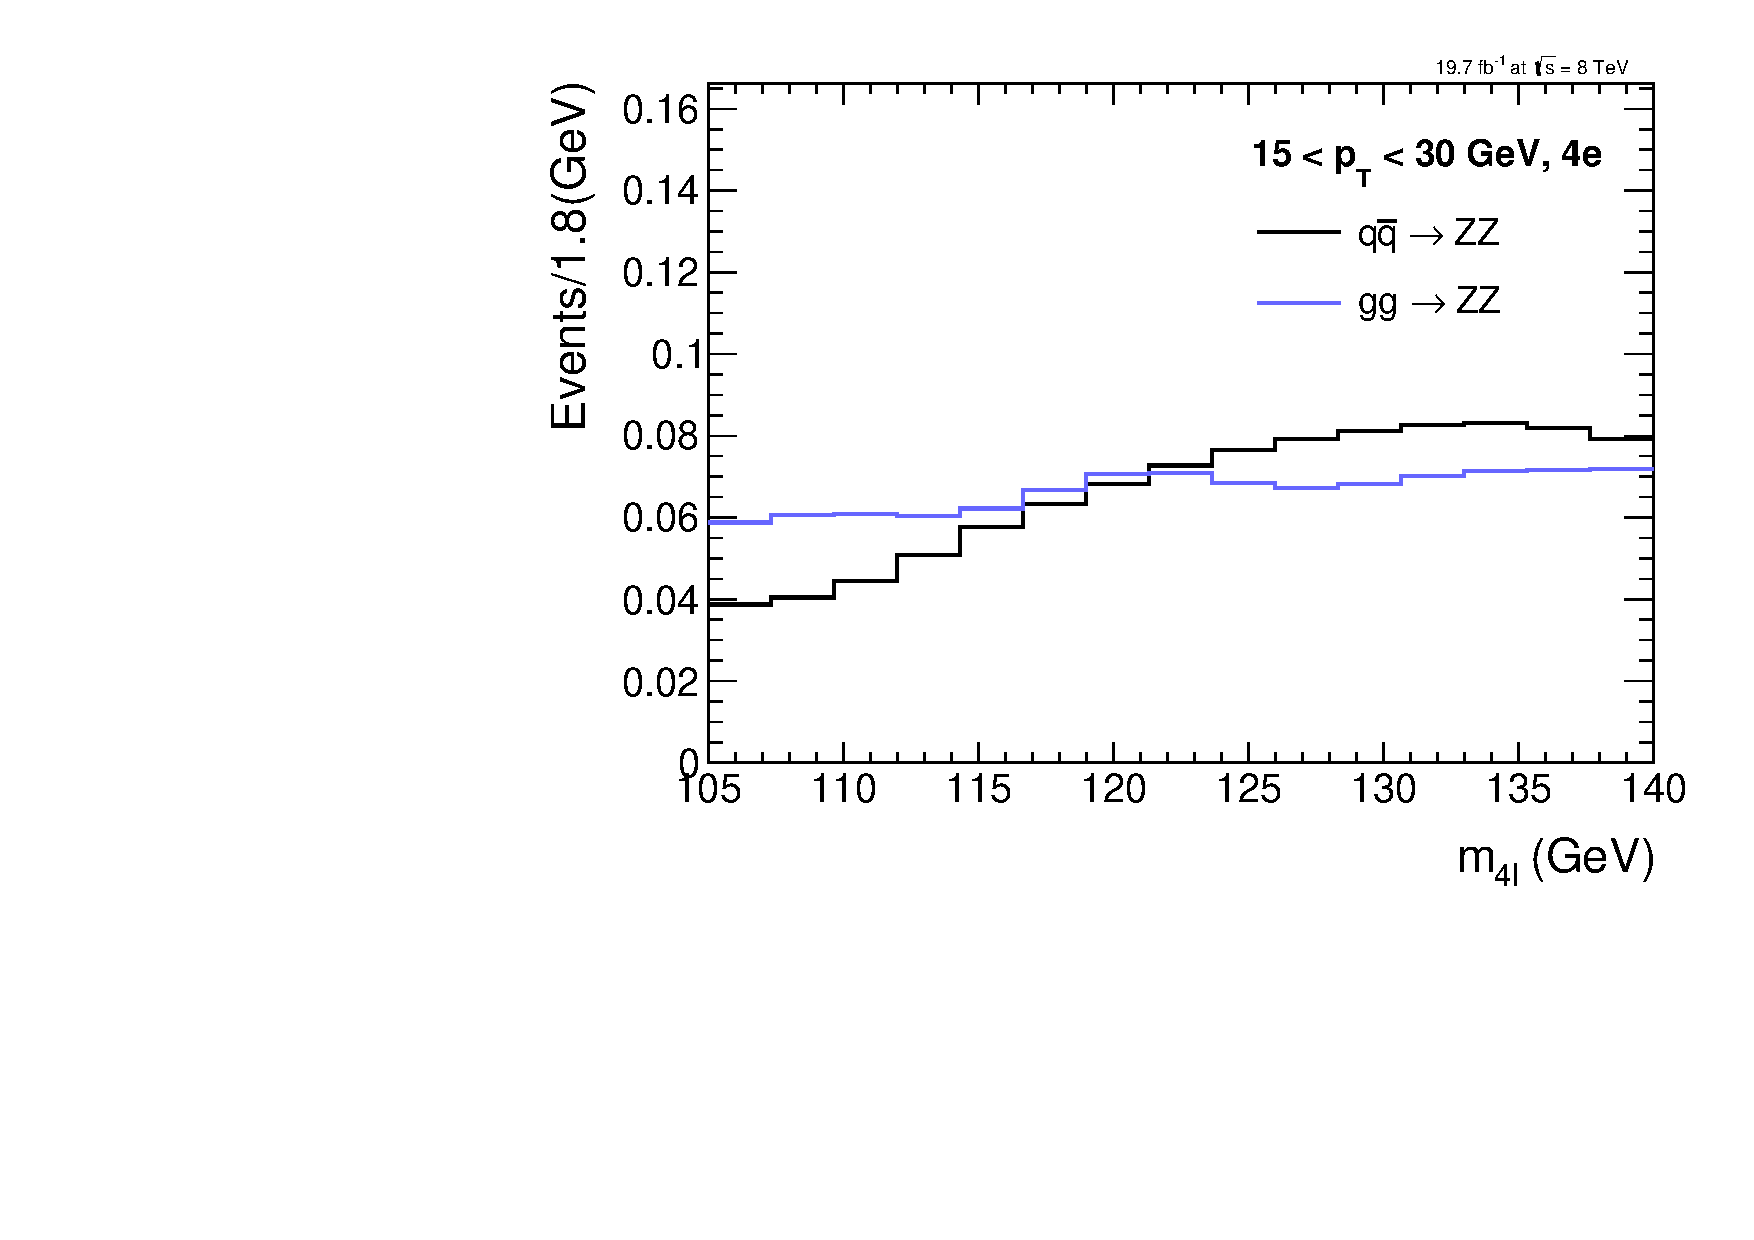
\includegraphics[width=0.30\textwidth,angle=0]{Appendix/figures/XSTemplates_4e_pT4l_15_30_qqZZ_ggZZ.pdf}
      \label{fig:bkg-pT4l-qqZZ-ggZZ-4e:b}
    } \\
    
    \subfigure[$30.0 \GeV < \pt(4\ell) < 60.0 \GeV$]{
      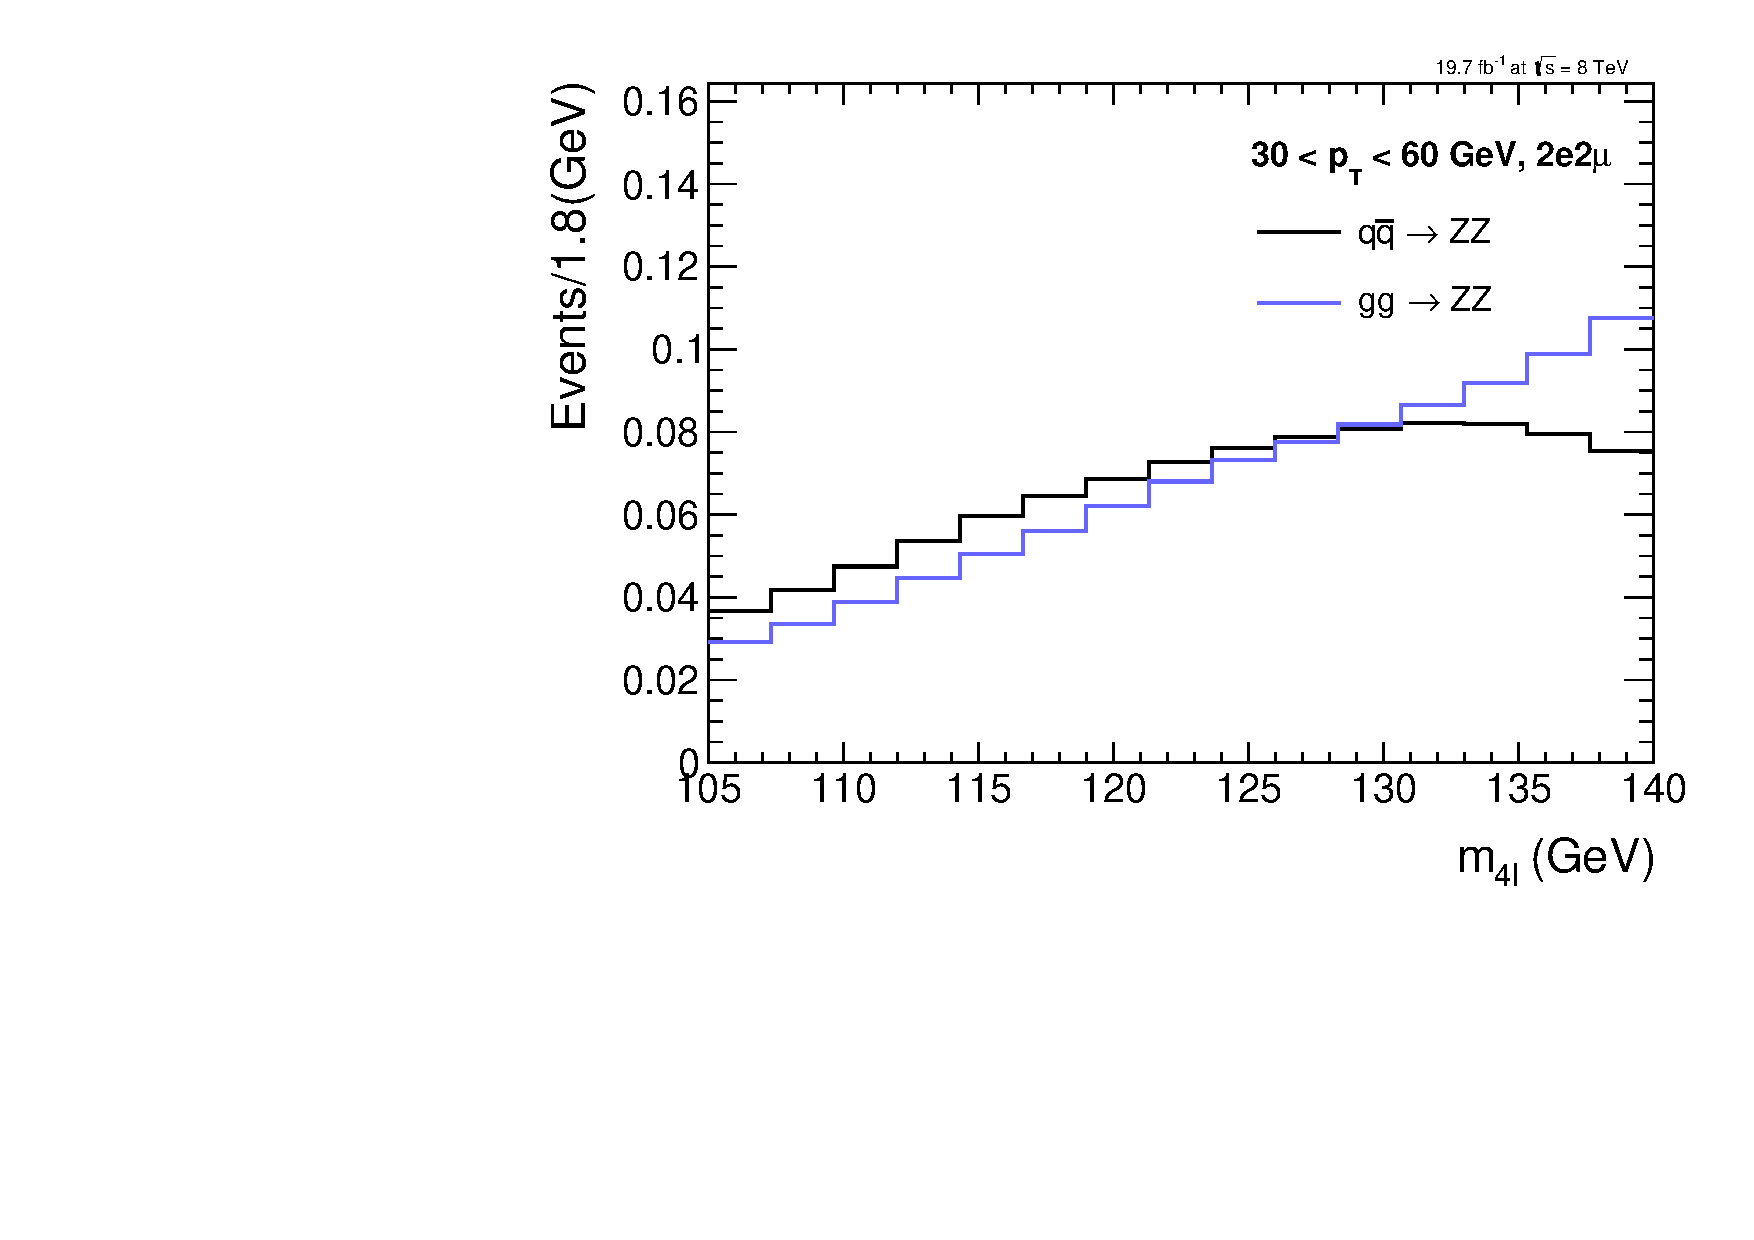
\includegraphics[width=0.30\textwidth,angle=0]{Appendix/figures/XSTemplates_2e2mu_pT4l_30_60_qqZZ_ggZZ.pdf}
      \label{fig:bkg-pT4l-qqZZ-ggZZ-2e2mu:c}
    }
    \subfigure[$30.0 \GeV < \pt(4\ell) < 60.0 \GeV$]{
      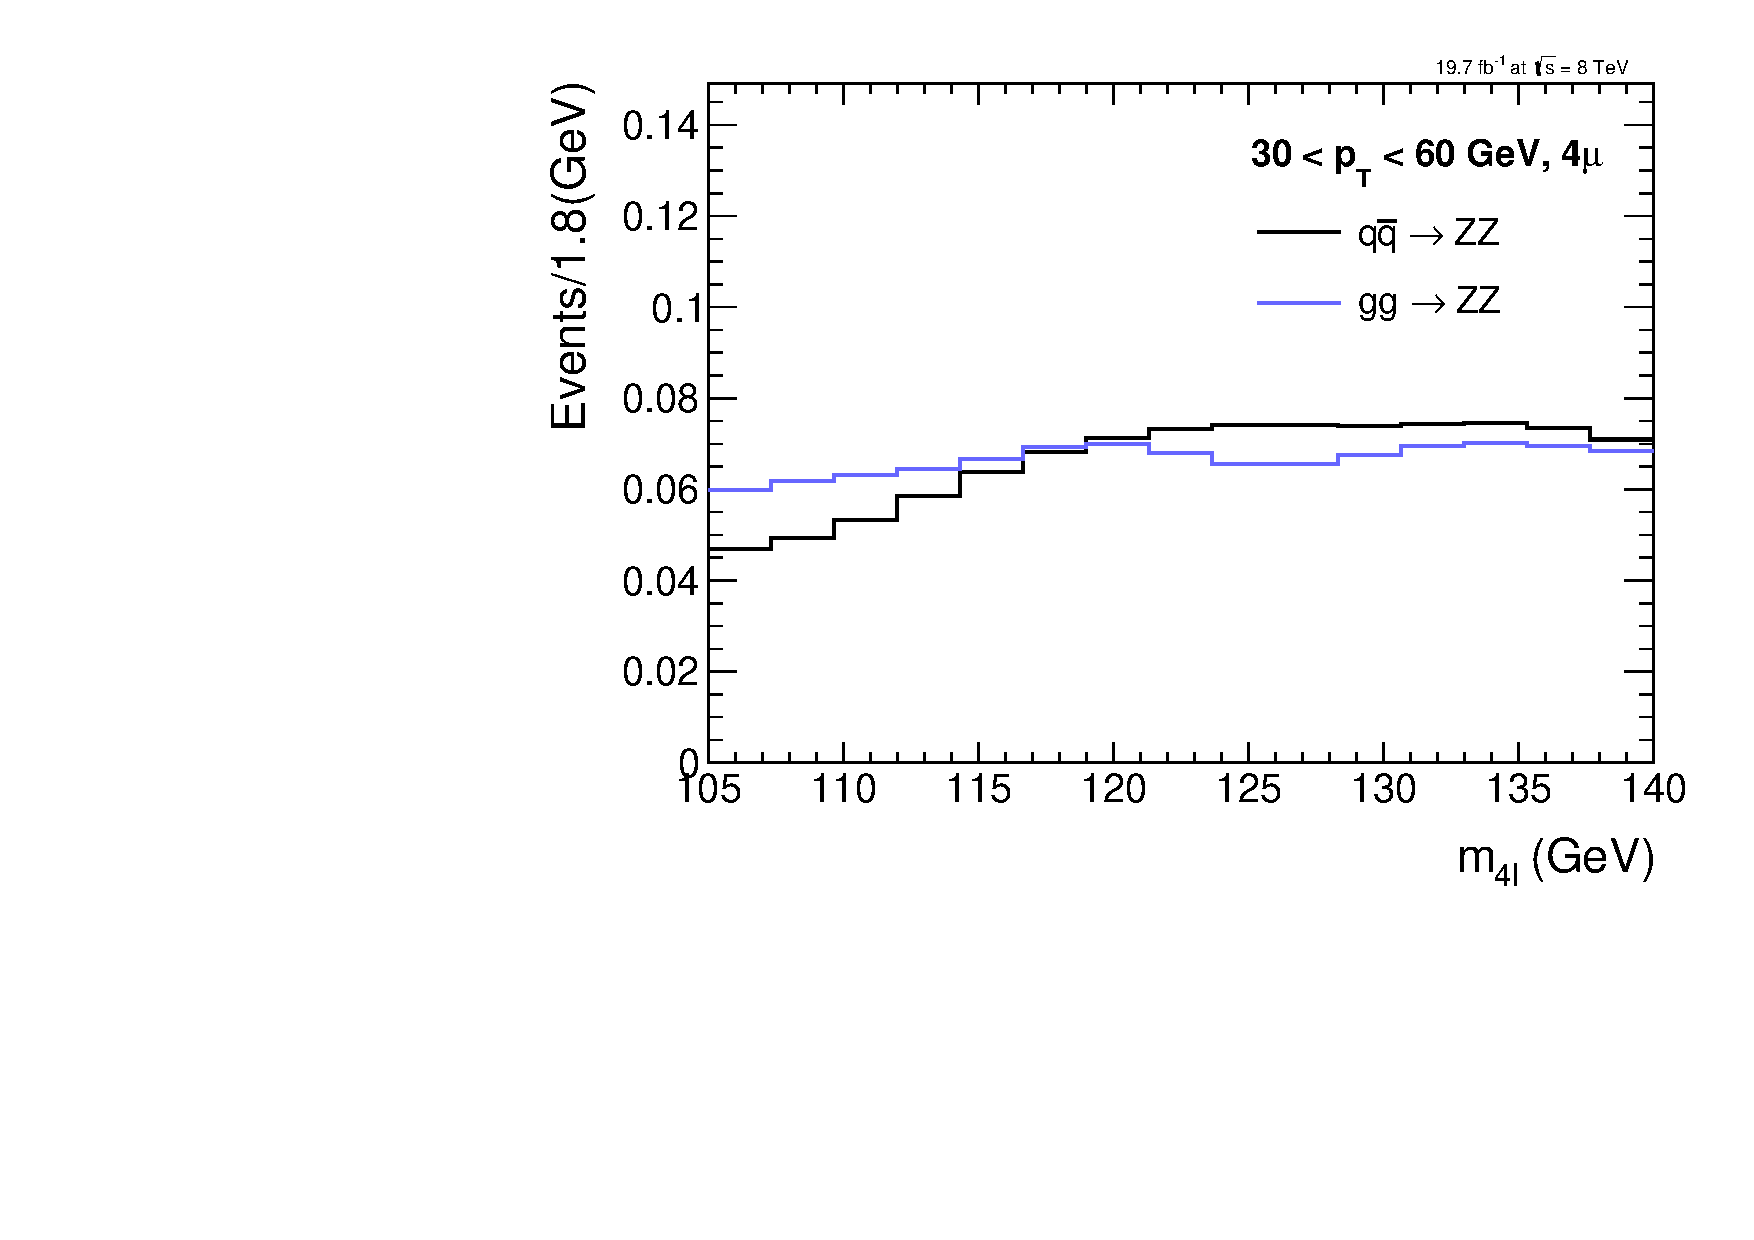
\includegraphics[width=0.30\textwidth,angle=0]{Appendix/figures/XSTemplates_4mu_pT4l_30_60_qqZZ_ggZZ.pdf}
      \label{fig:bkg-pT4l-qqZZ-ggZZ-4mu:c}
    }
    \subfigure[$30.0 \GeV < \pt(4\ell) < 60.0 \GeV$]{
      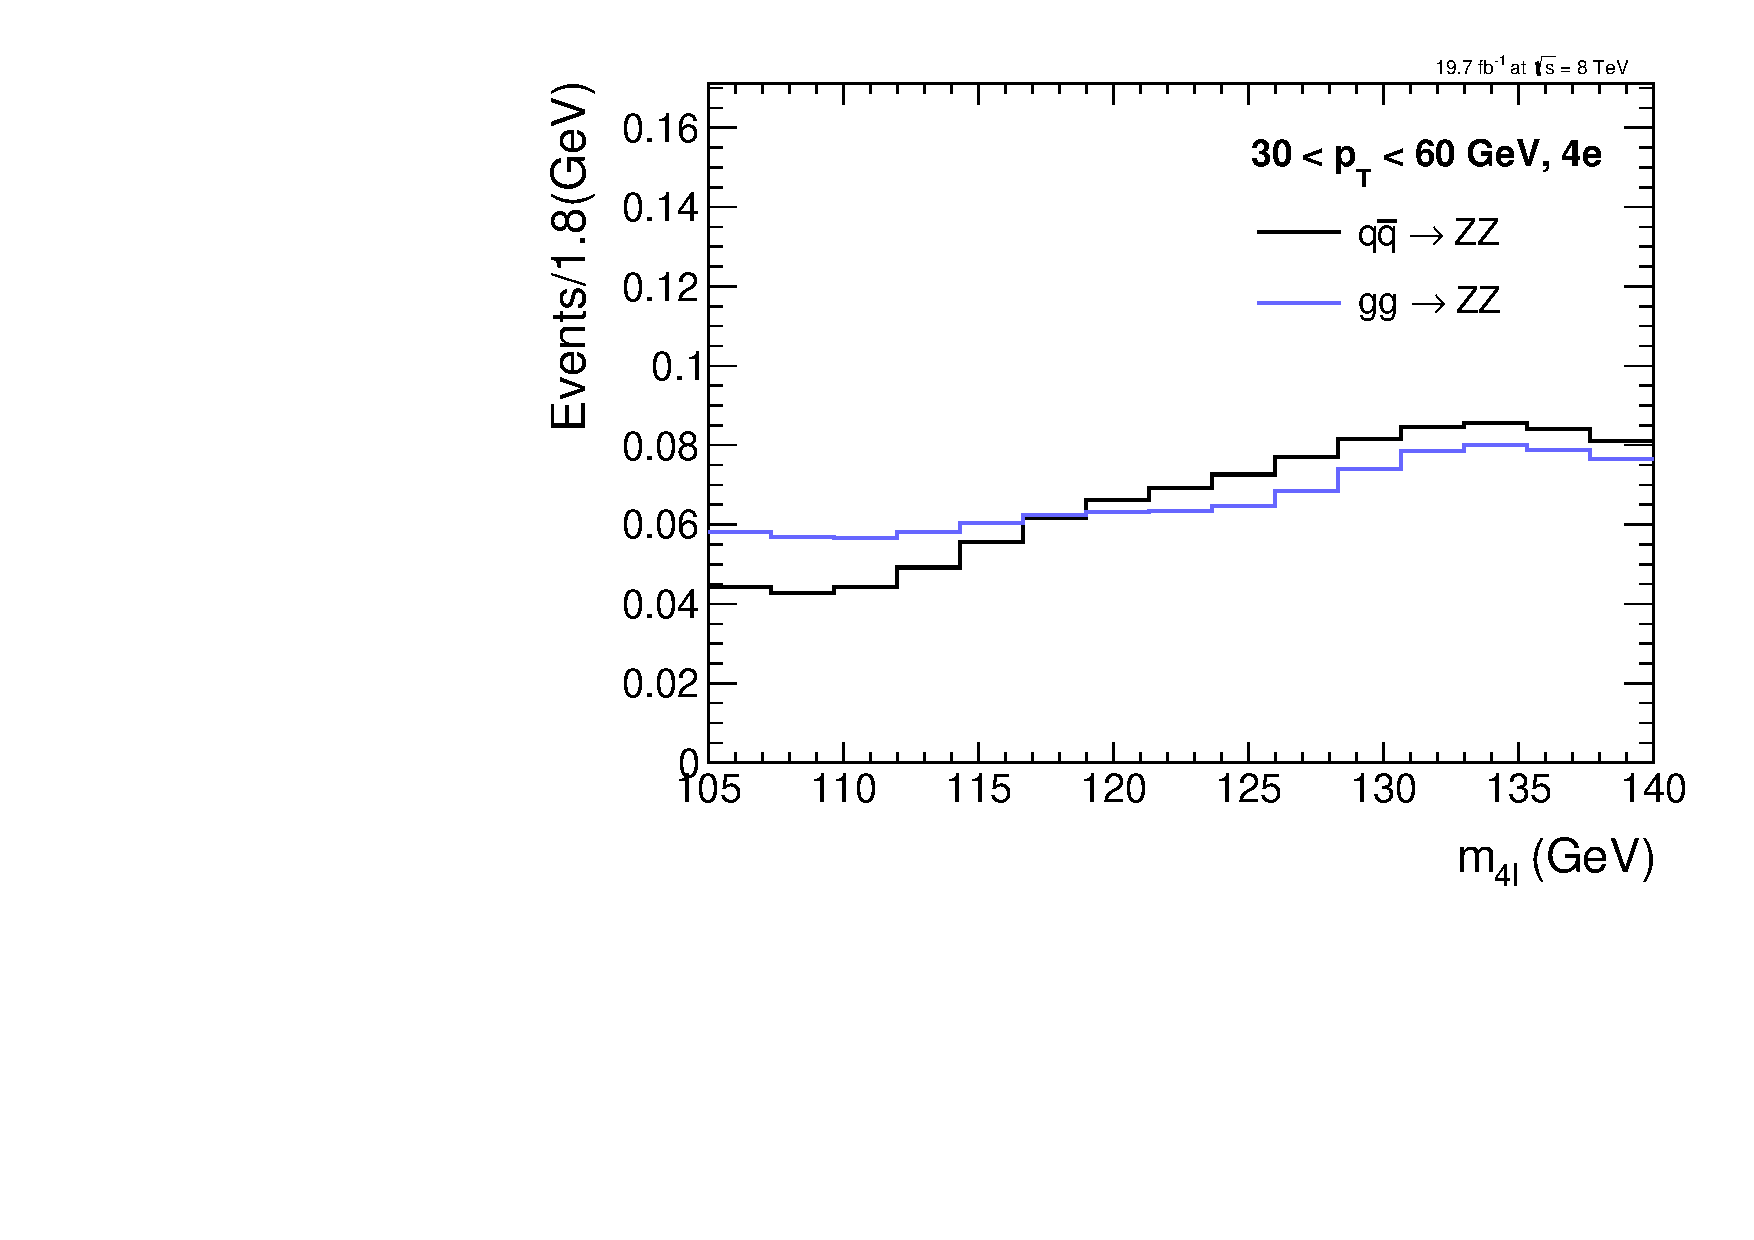
\includegraphics[width=0.30\textwidth,angle=0]{Appendix/figures/XSTemplates_4e_pT4l_30_60_qqZZ_ggZZ.pdf}
      \label{fig:bkg-pT4l-qqZZ-ggZZ-4e:c}
    } \\
    
    \subfigure[$60.0 \GeV < \pt(4\ell) < 1000.0 \GeV$]{
      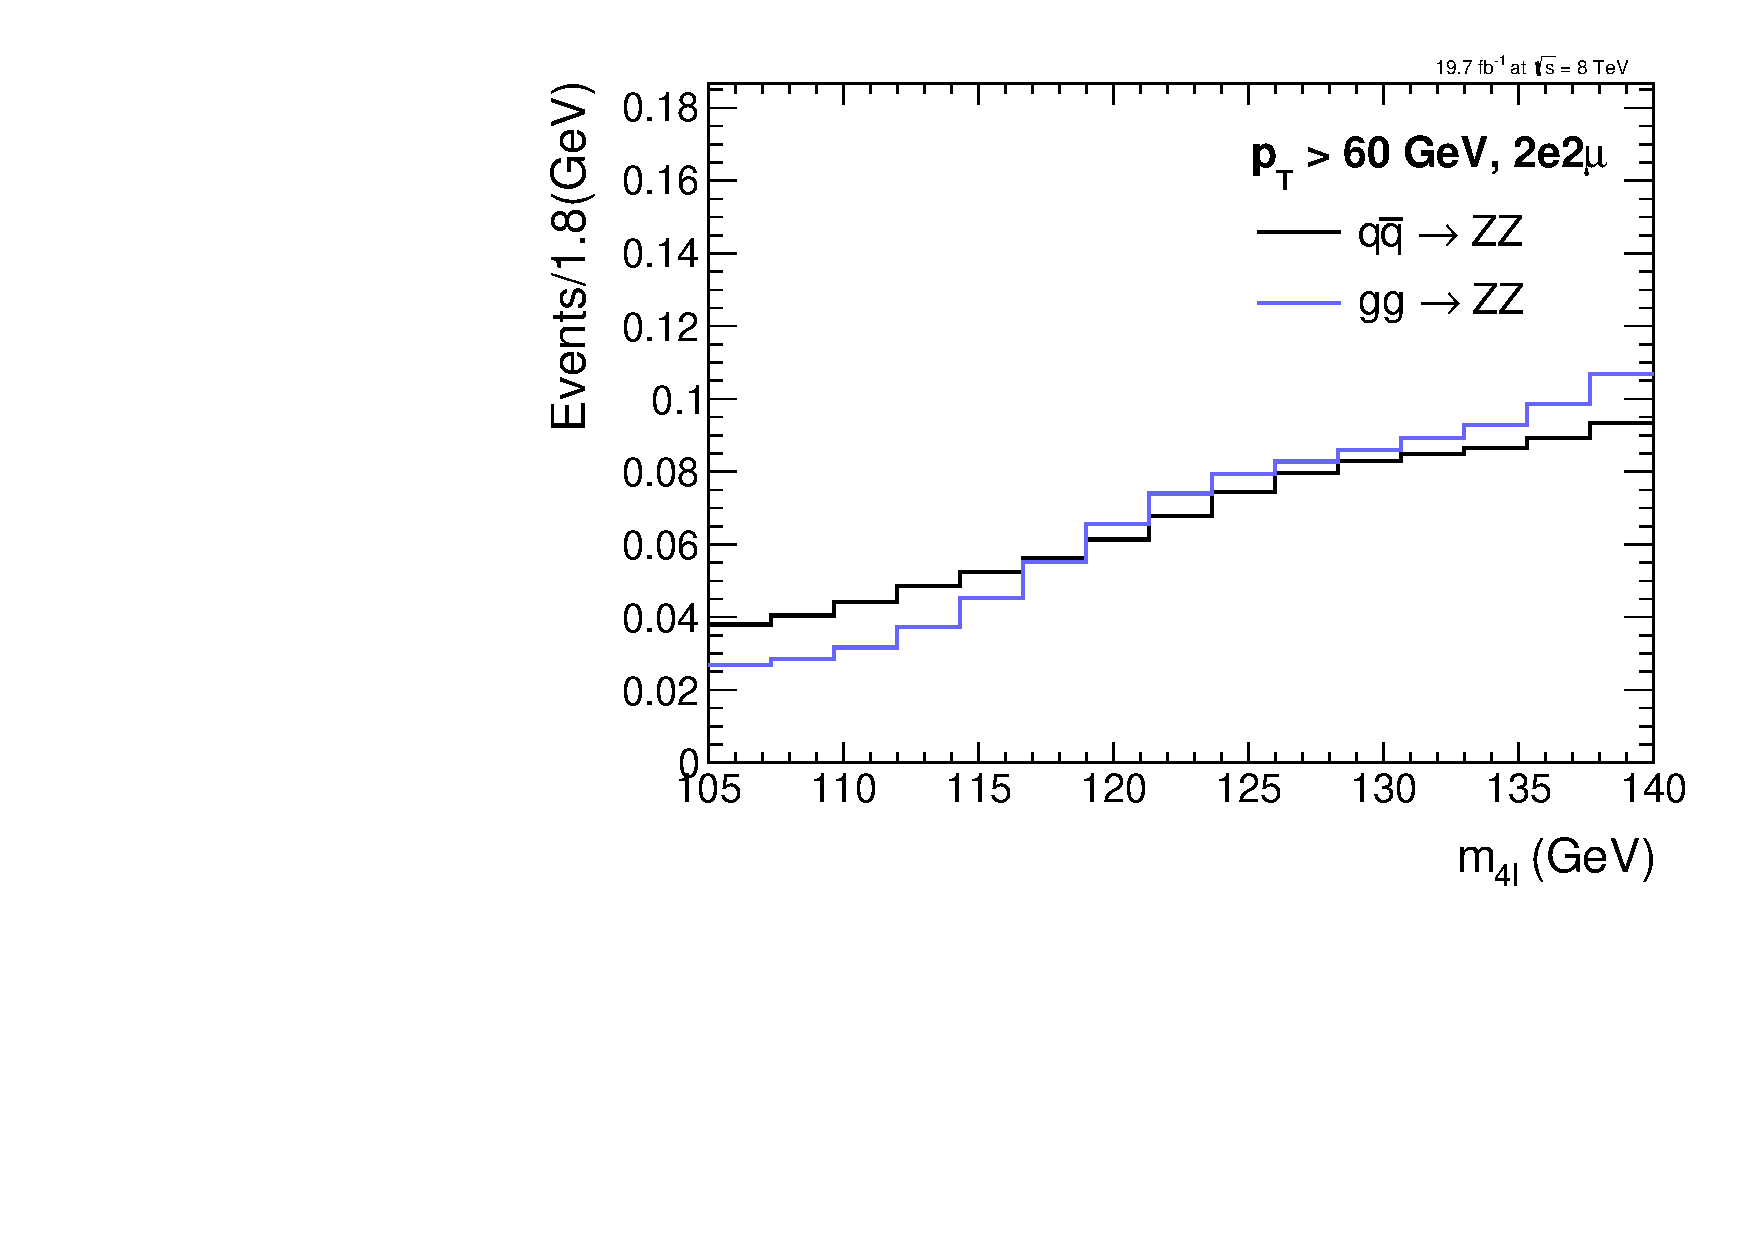
\includegraphics[width=0.30\textwidth,angle=0]{Appendix/figures/XSTemplates_2e2mu_pT4l_60_200_qqZZ_ggZZ.pdf}
      \label{fig:bkg-pT4l-qqZZ-ggZZ-2e2mu:d}
    }
    \subfigure[$60.0 \GeV < \pt(4\ell) < 1000.0 \GeV$]{
      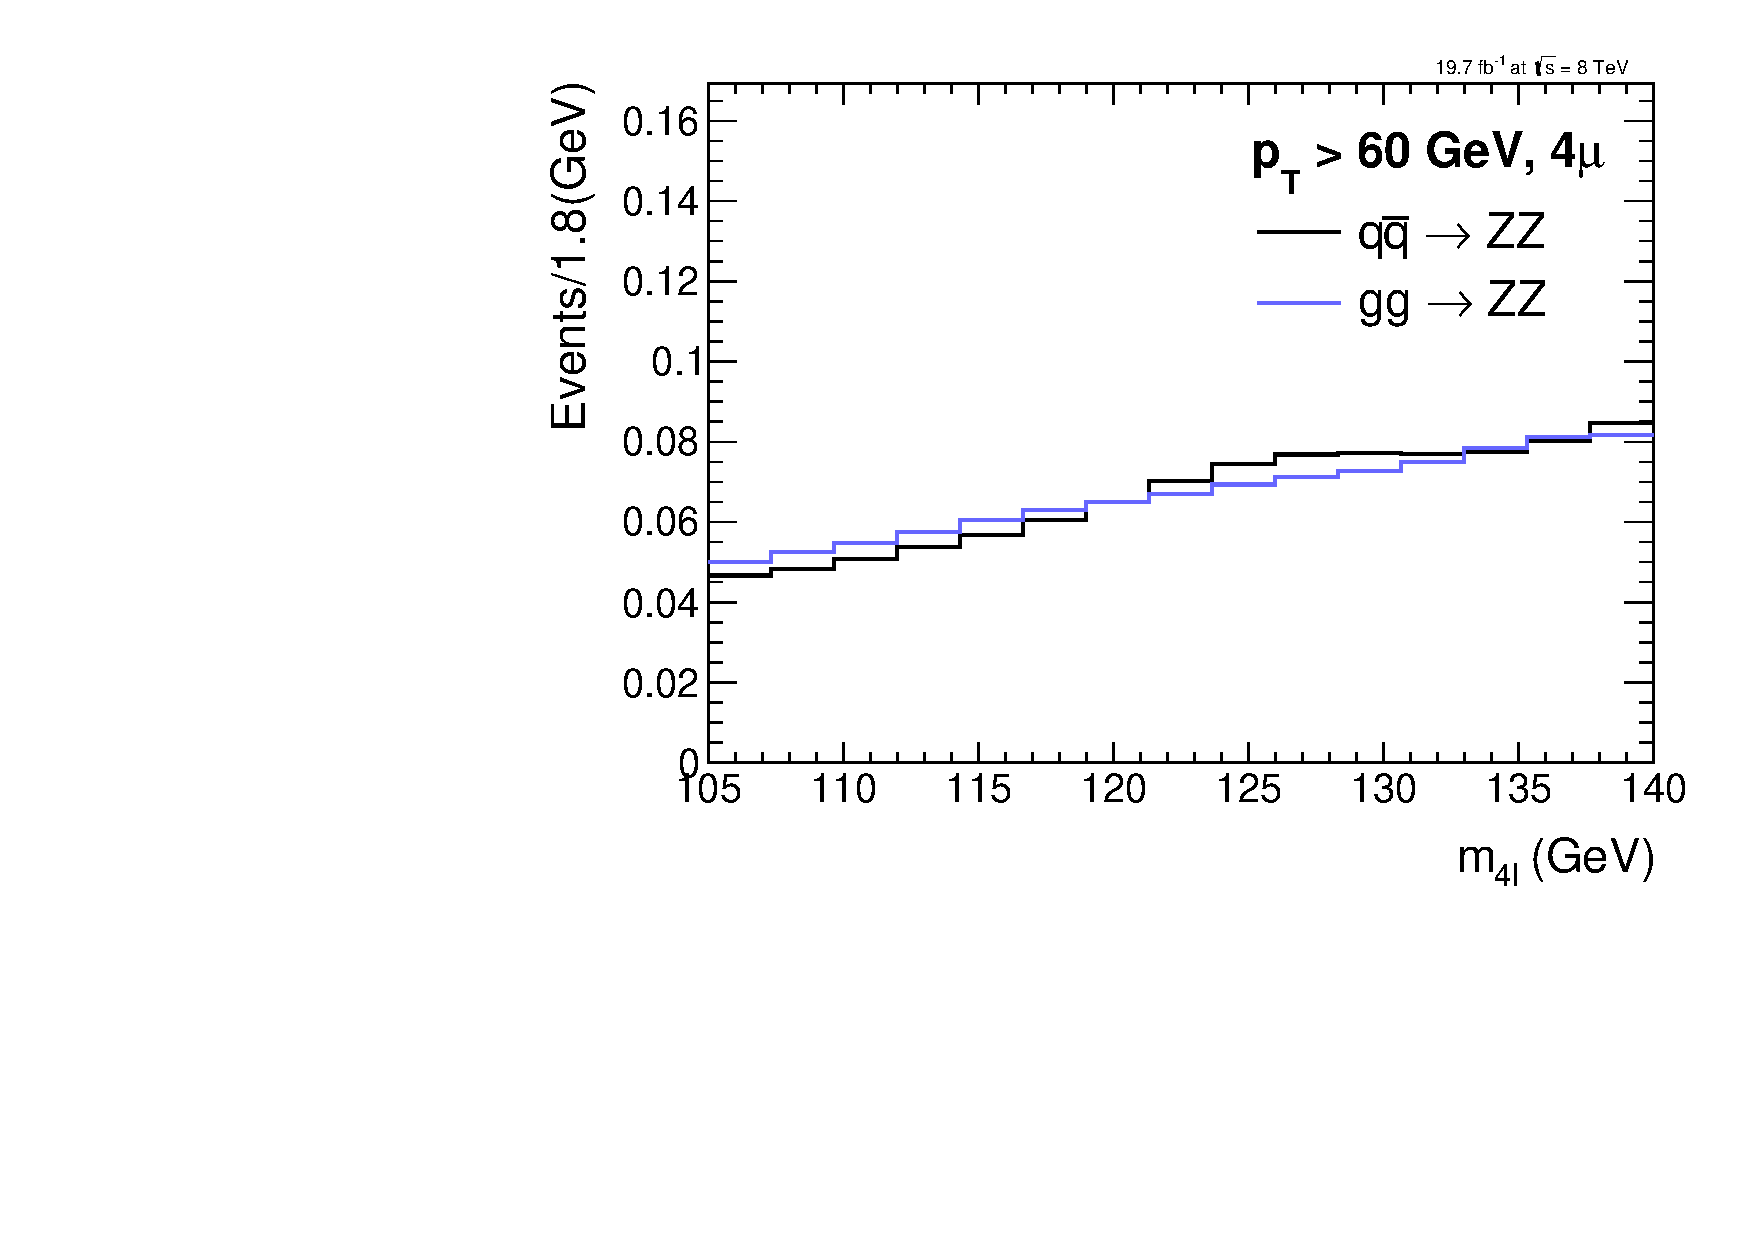
\includegraphics[width=0.30\textwidth,angle=0]{Appendix/figures/XSTemplates_4mu_pT4l_60_200_qqZZ_ggZZ.pdf}
      \label{fig:bkg-pT4l-qqZZ-ggZZ-4mu:d}
    }
    \subfigure[$60.0 \GeV < \pt(4\ell) < 1000.0 \GeV$]{
      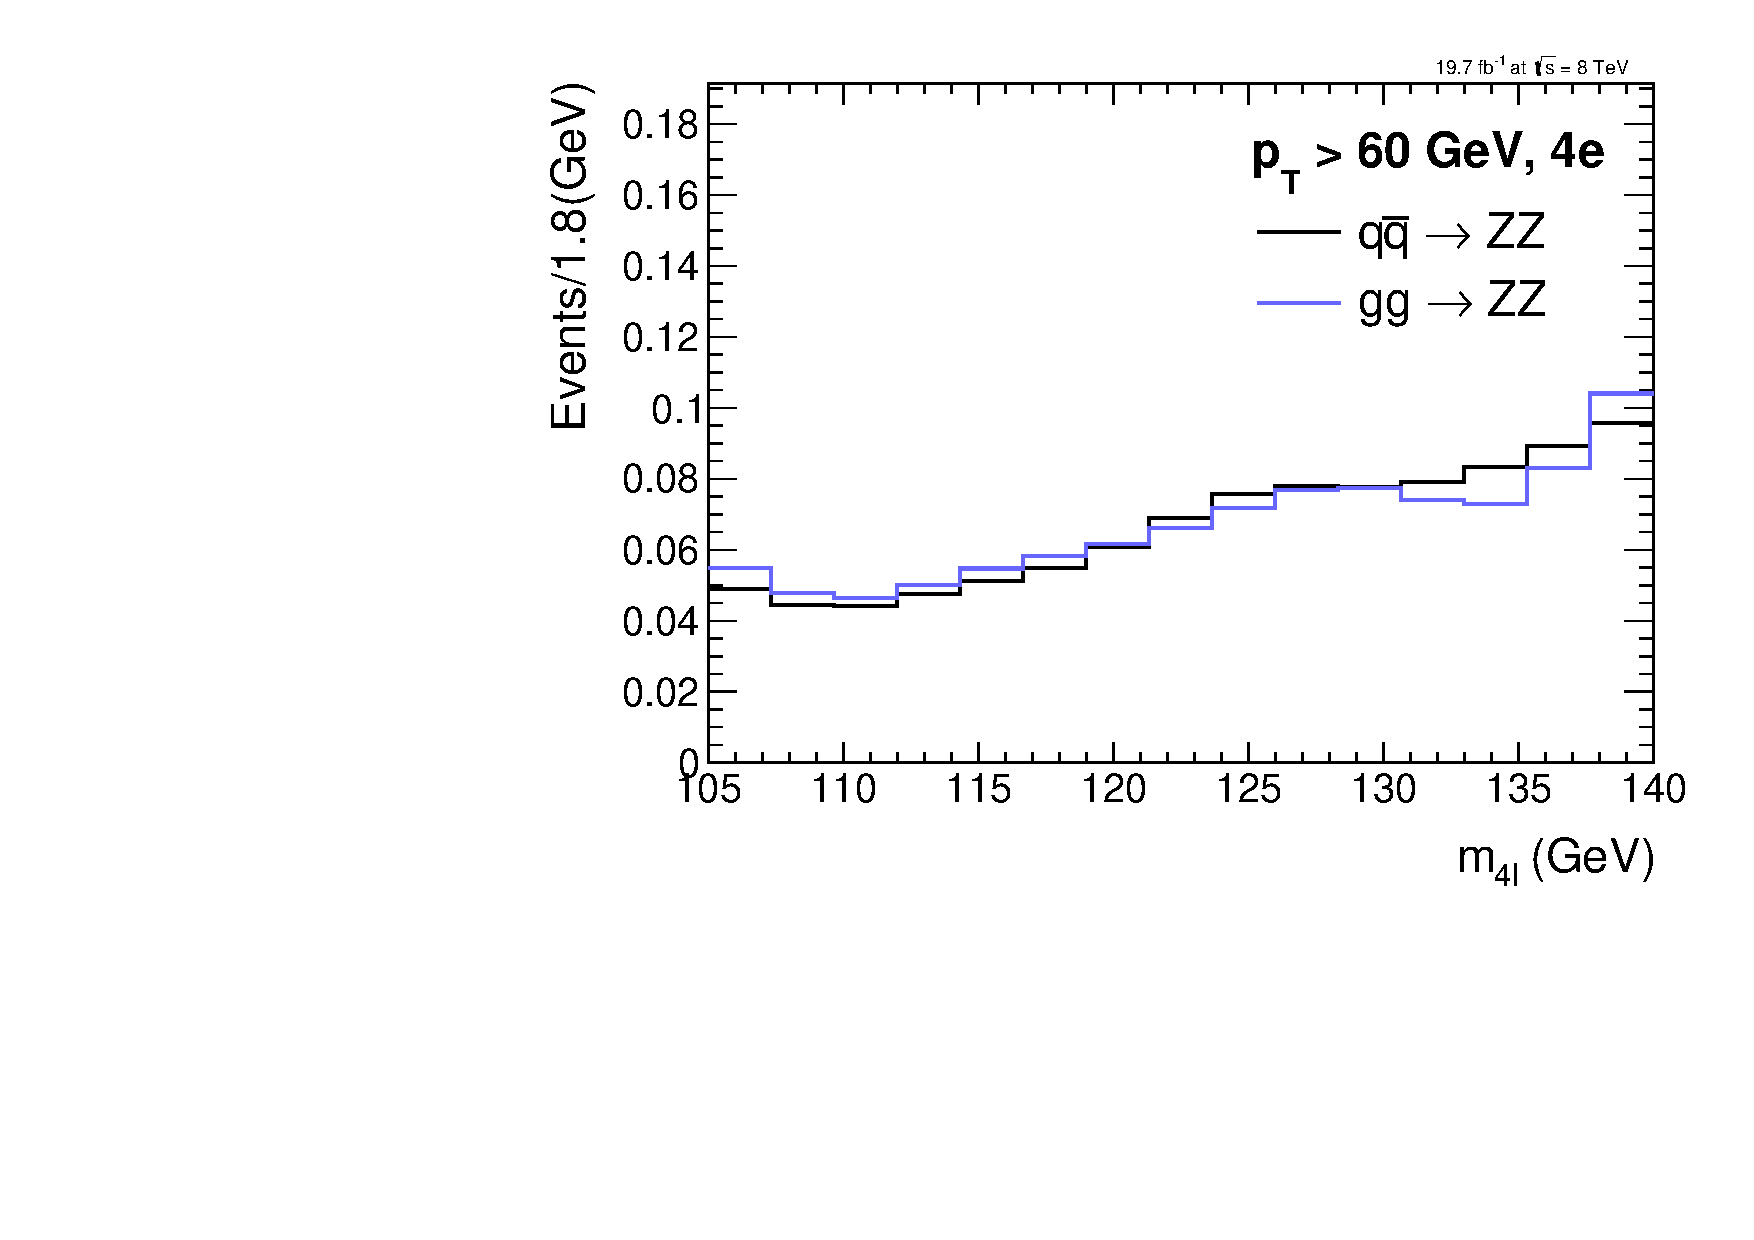
\includegraphics[width=0.30\textwidth,angle=0]{Appendix/figures/XSTemplates_4e_pT4l_60_200_qqZZ_ggZZ.pdf}
      \label{fig:bkg-pT4l-qqZZ-ggZZ-4e:d}
    } \\
    
    \caption{ Distributions of m($4\ell$) for the $qq \rightarrow \mathrm{ZZ}$ and $gg \rightarrow \mathrm{ZZ}$ backgrounds 
    in different bins of $\pt(4\ell)$ for three final states: $2e2\mu$(left), $4\mu$(middle) and $4e$(right).}
  \label{fig:bkg-pT4l-qqZZ-ggZZ}
  
 \end{center}
\end{figure} 

\clearpage

\subsection[Mass of the second Z boson]{Background shapes in bins of $m(\mathrm{Z}_{2})$ }

\begin{figure}[!ht]
  \begin{center}
  
    \subfigure[$12.0 \GeV < \mathrm{m}(\mathrm{Z}_{2}) < 20.0 \GeV$]{
      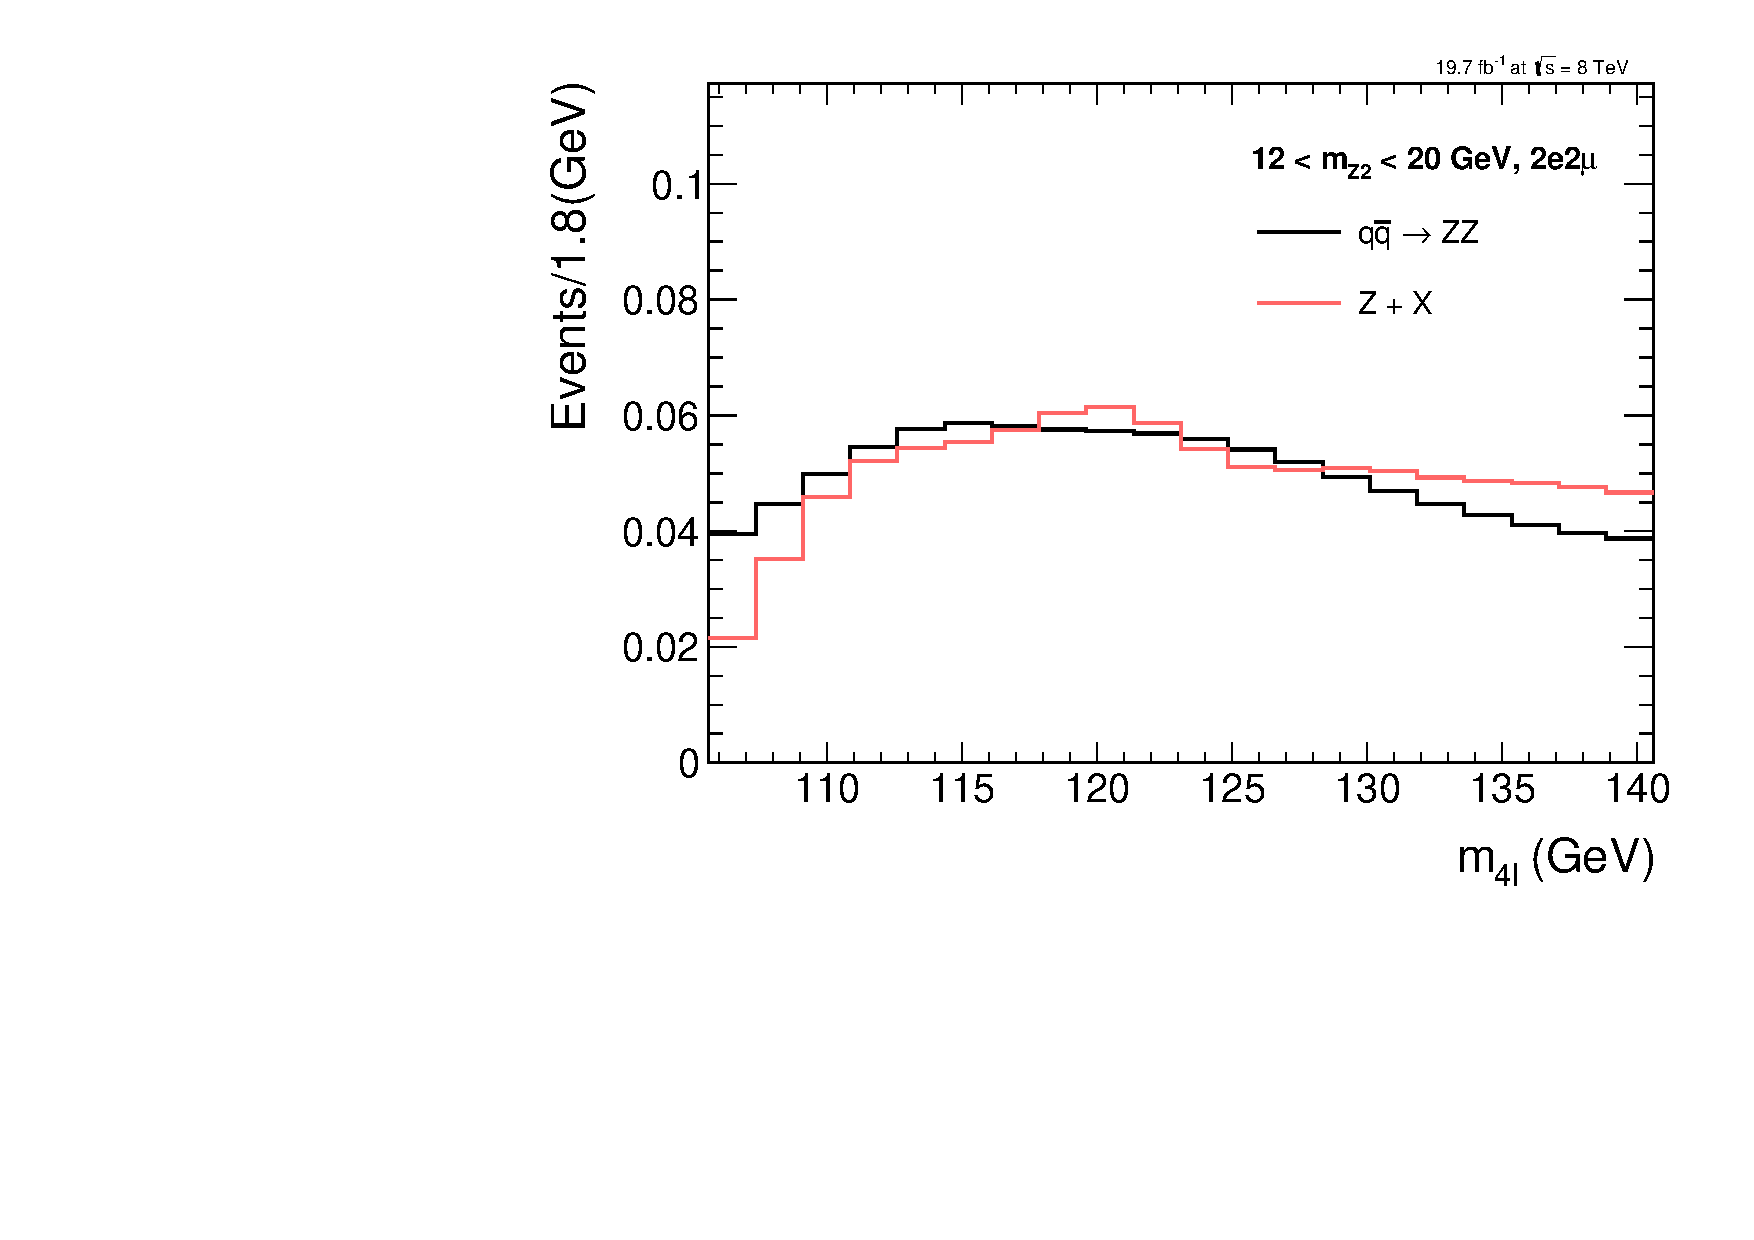
\includegraphics[width=0.30\textwidth,angle=0]{Appendix/figures/XSTemplates_2e2mu_massZ2_12_20_qqZZ_ZJetsCR.pdf}
      \label{fig:bkg-massZ2-qqZZ-ZX-2e2mu:a}
    }    
    \subfigure[$12.0 \GeV < \mathrm{m}(\mathrm{Z}_{2}) < 20.0 \GeV$]{
      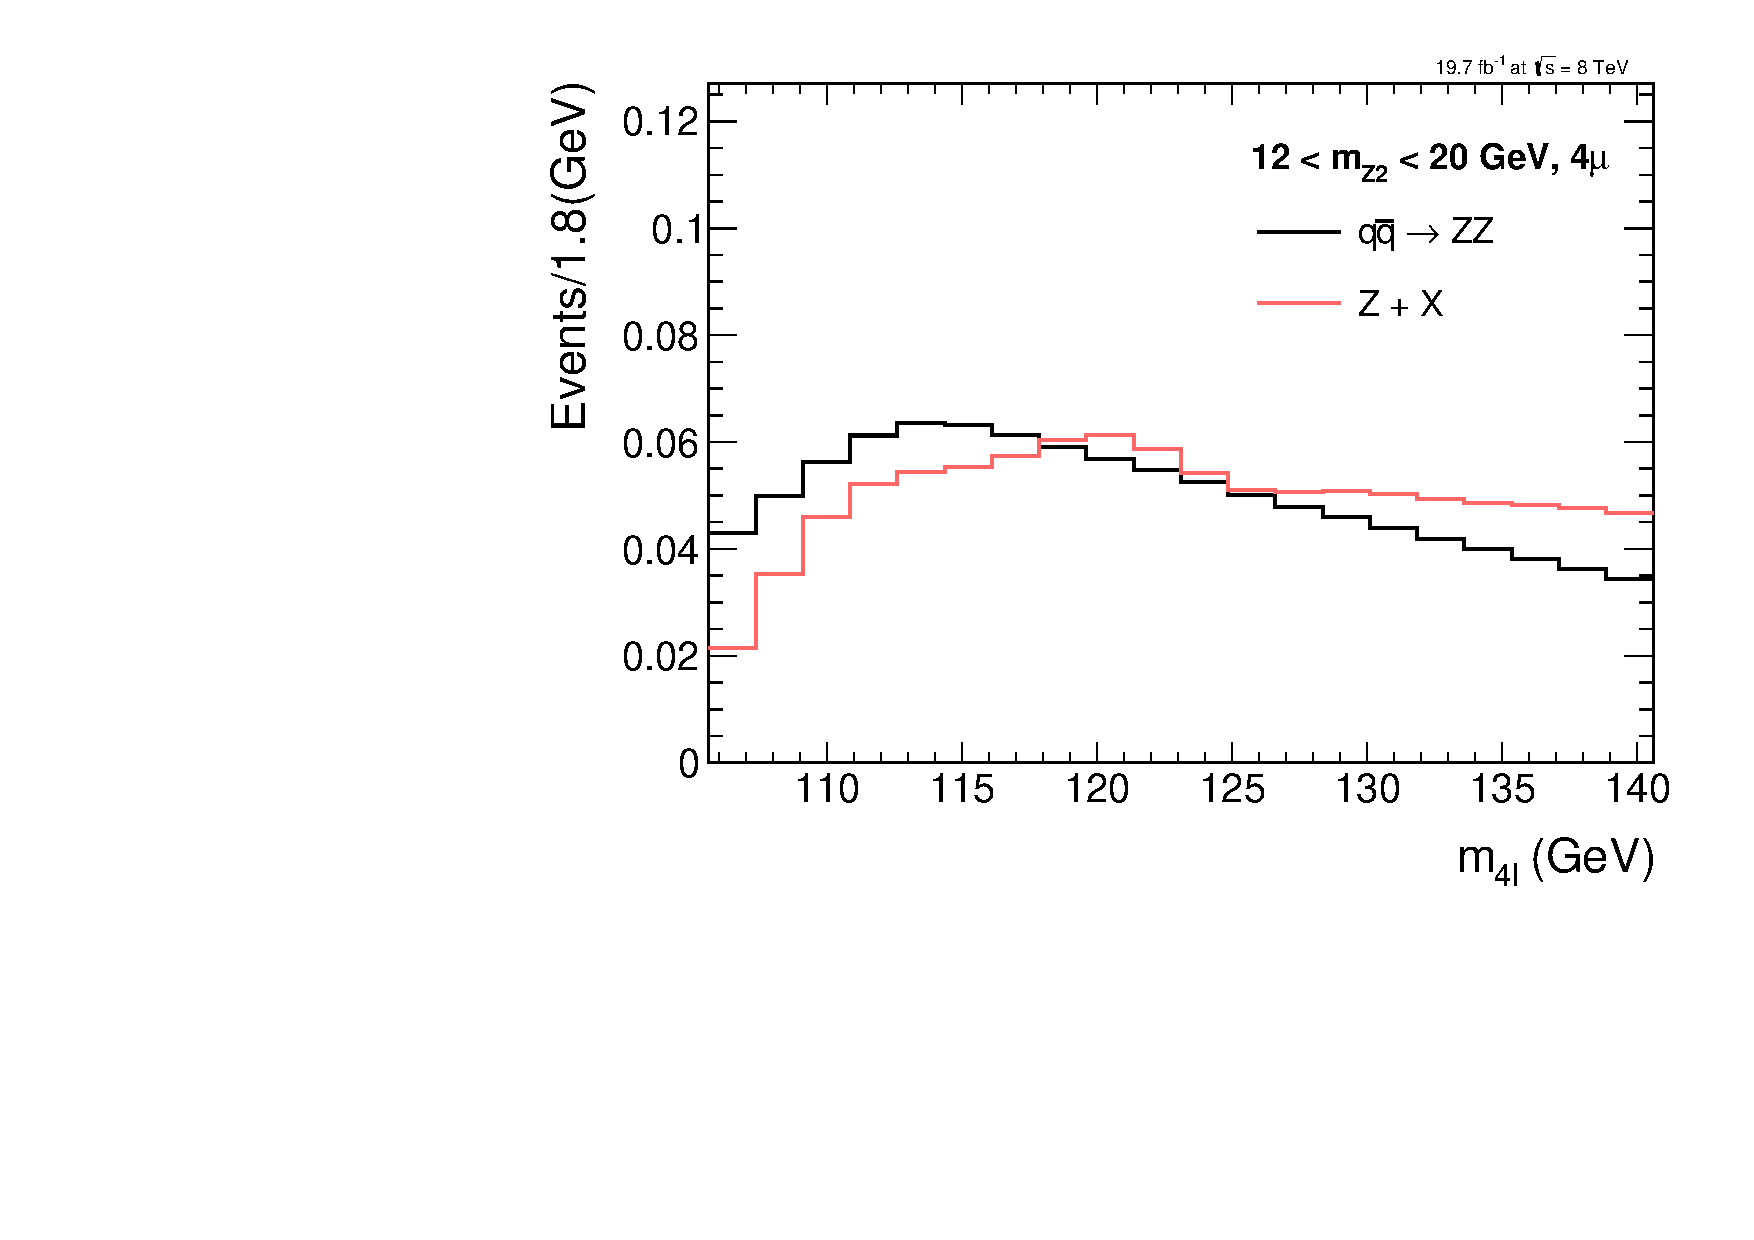
\includegraphics[width=0.30\textwidth,angle=0]{Appendix/figures/XSTemplates_4mu_massZ2_12_20_qqZZ_ZJetsCR.pdf}
      \label{fig:bkg-massZ2-qqZZ-ZX-4mu:a}
    }    
    \subfigure[$12.0 \GeV < \mathrm{m}(\mathrm{Z}_{2}) < 20.0 \GeV$]{
      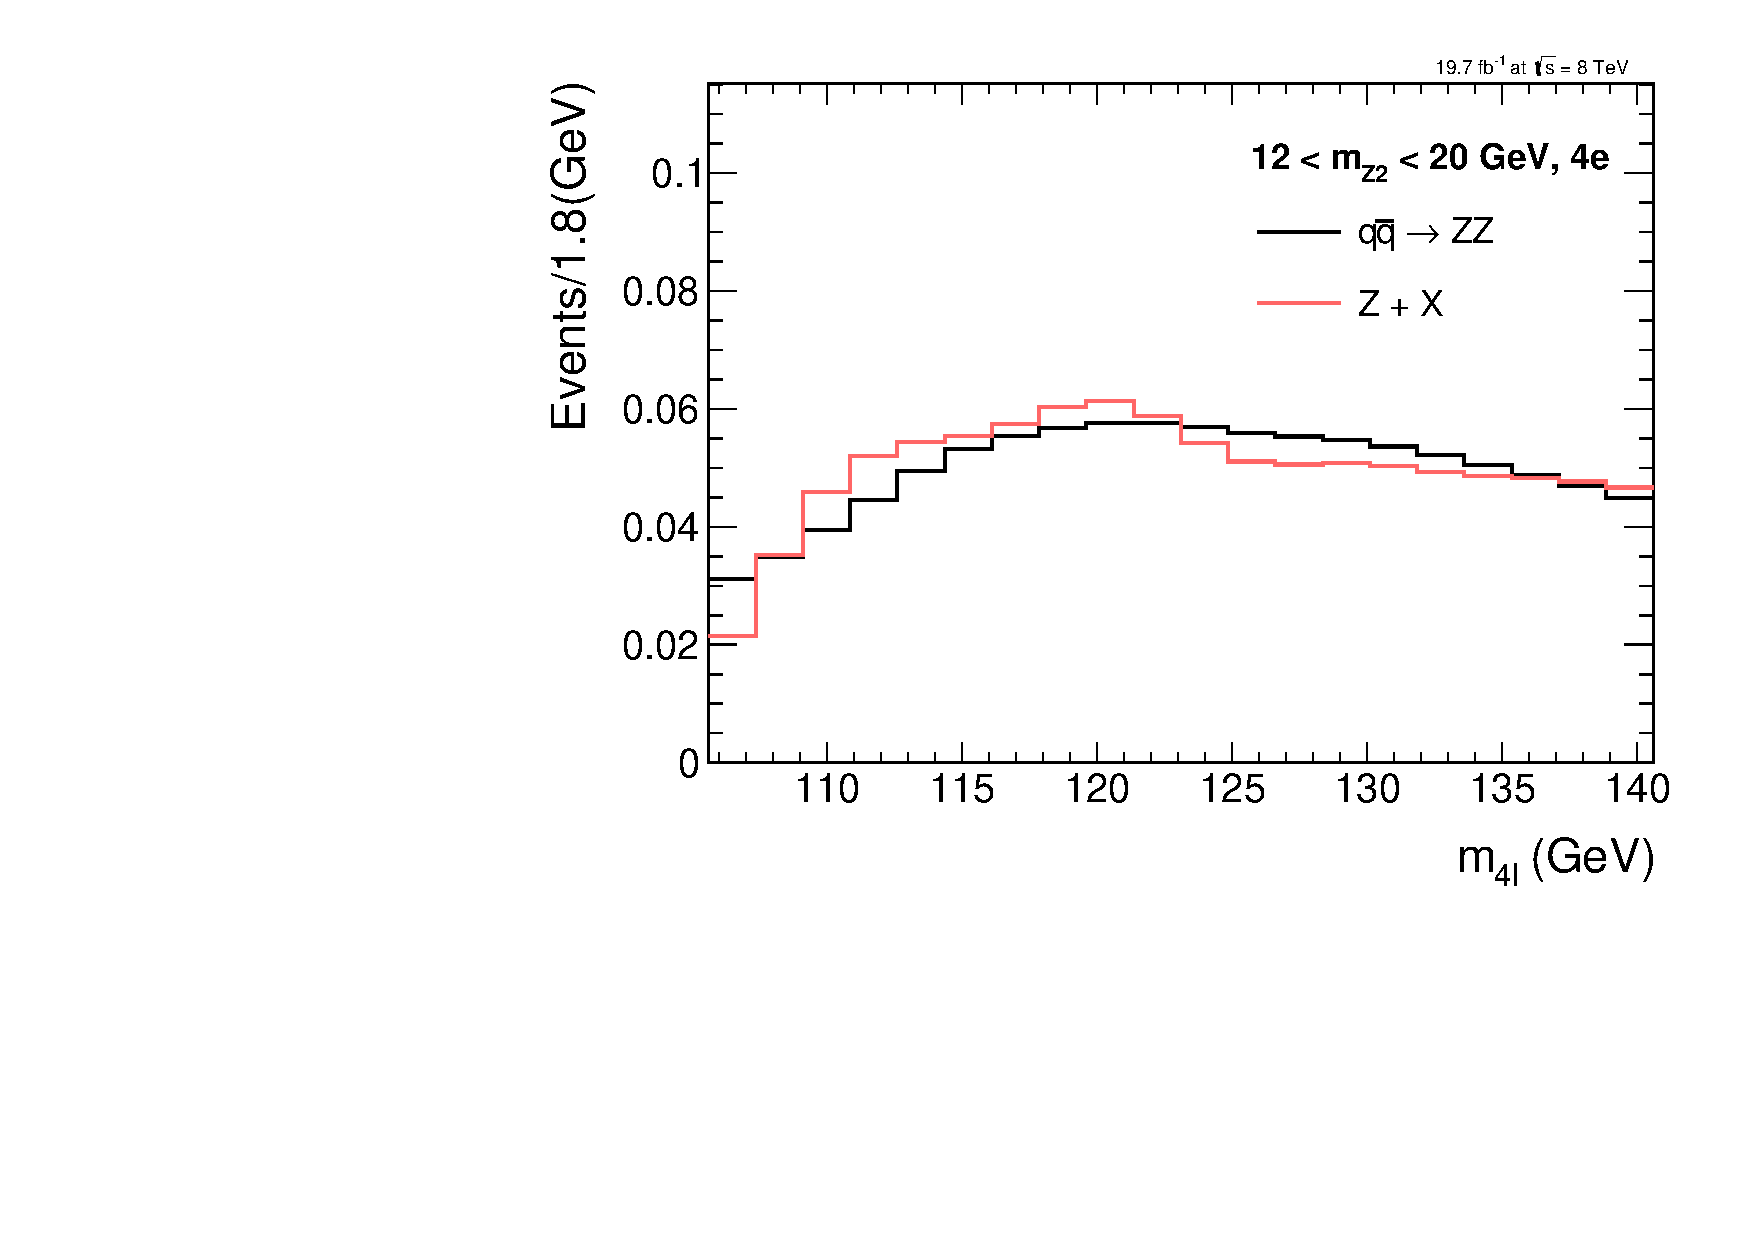
\includegraphics[width=0.30\textwidth,angle=0]{Appendix/figures/XSTemplates_4e_massZ2_12_20_qqZZ_ZJetsCR.pdf}
      \label{fig:bkg-massZ2-qqZZ-ZX-4e:a}
    }    \\

    \subfigure[$20.0 \GeV < \mathrm{m}(\mathrm{Z}_{2}) < 28.0 \GeV$]{
      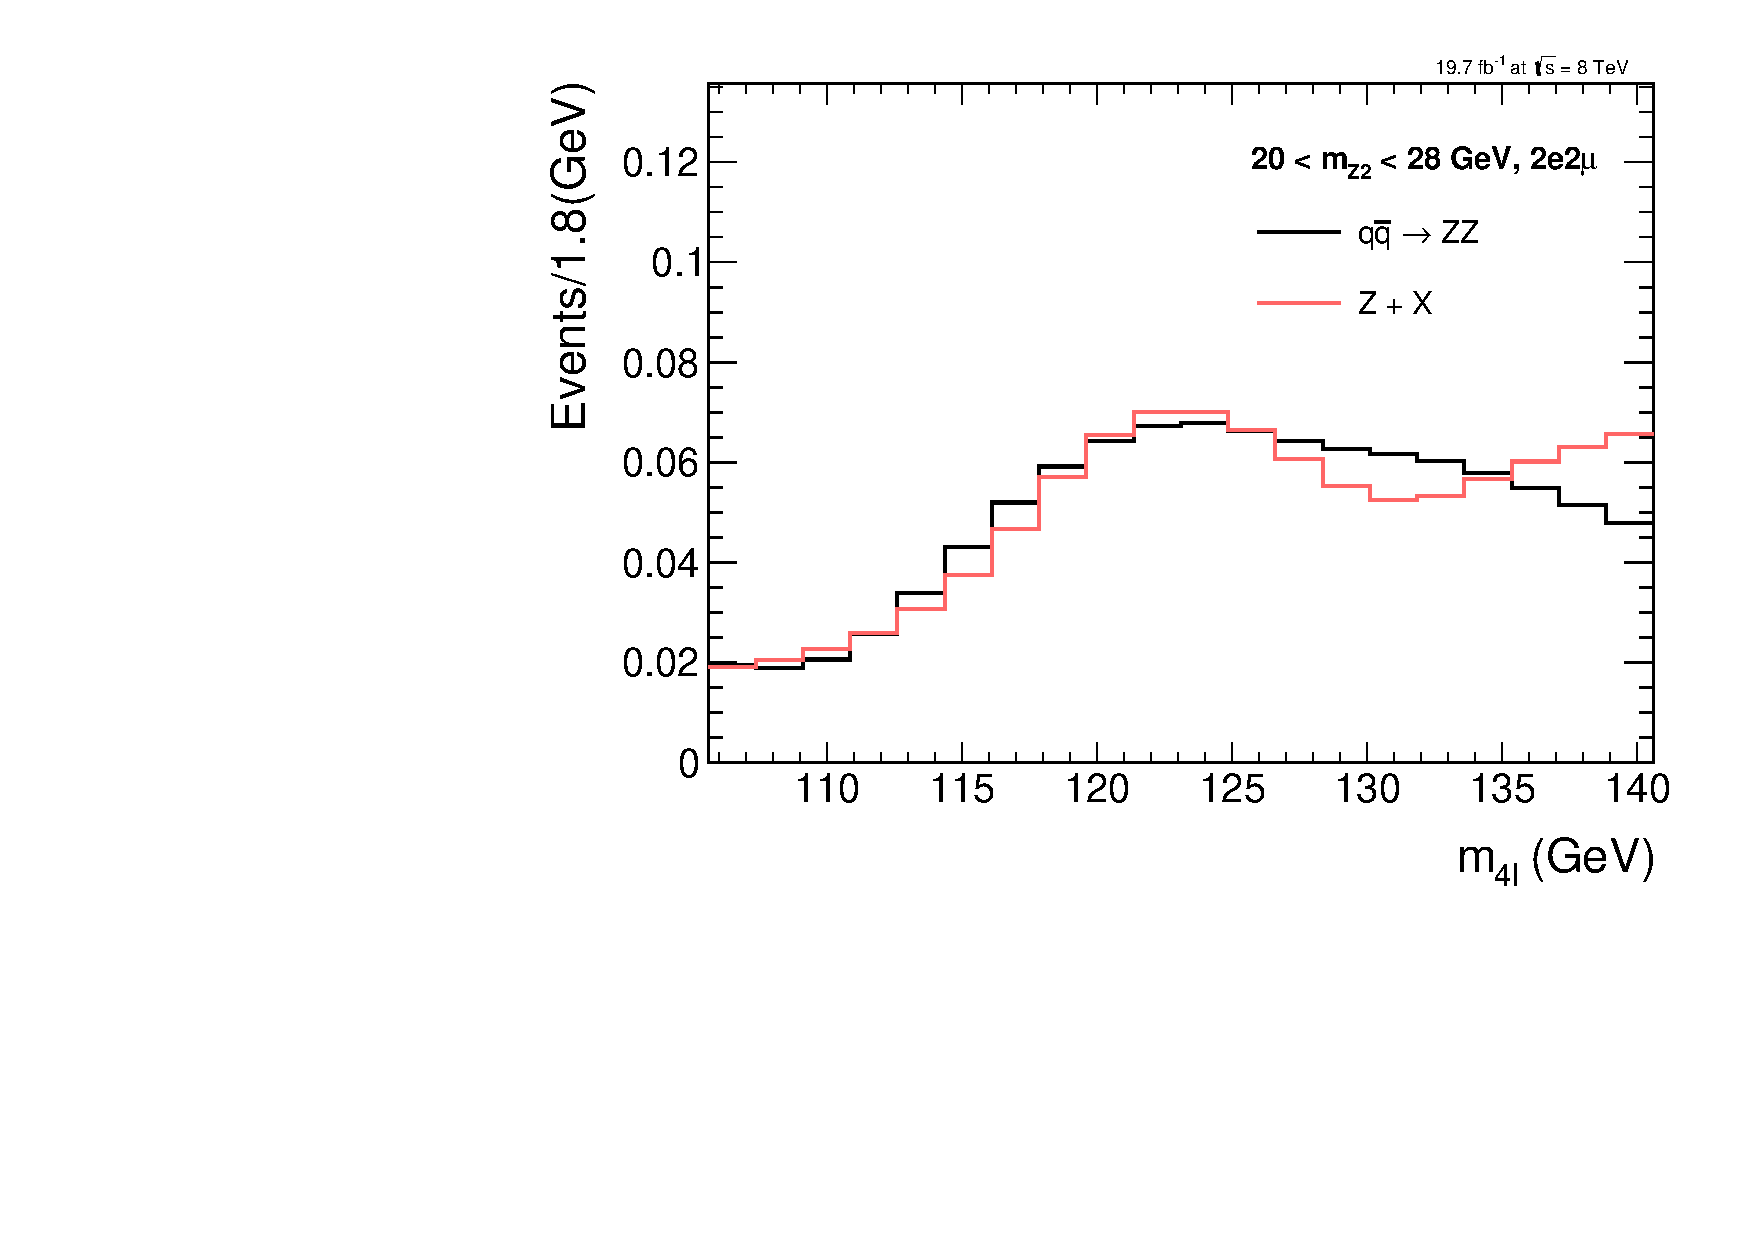
\includegraphics[width=0.30\textwidth,angle=0]{Appendix/figures/XSTemplates_2e2mu_massZ2_20_28_qqZZ_ZJetsCR.pdf}
      \label{fig:bkg-massZ2-qqZZ-ZX-2e2mu:b}
    }
    \subfigure[$20.0 \GeV < \mathrm{m}(\mathrm{Z}_{2}) < 28.0 \GeV$]{
      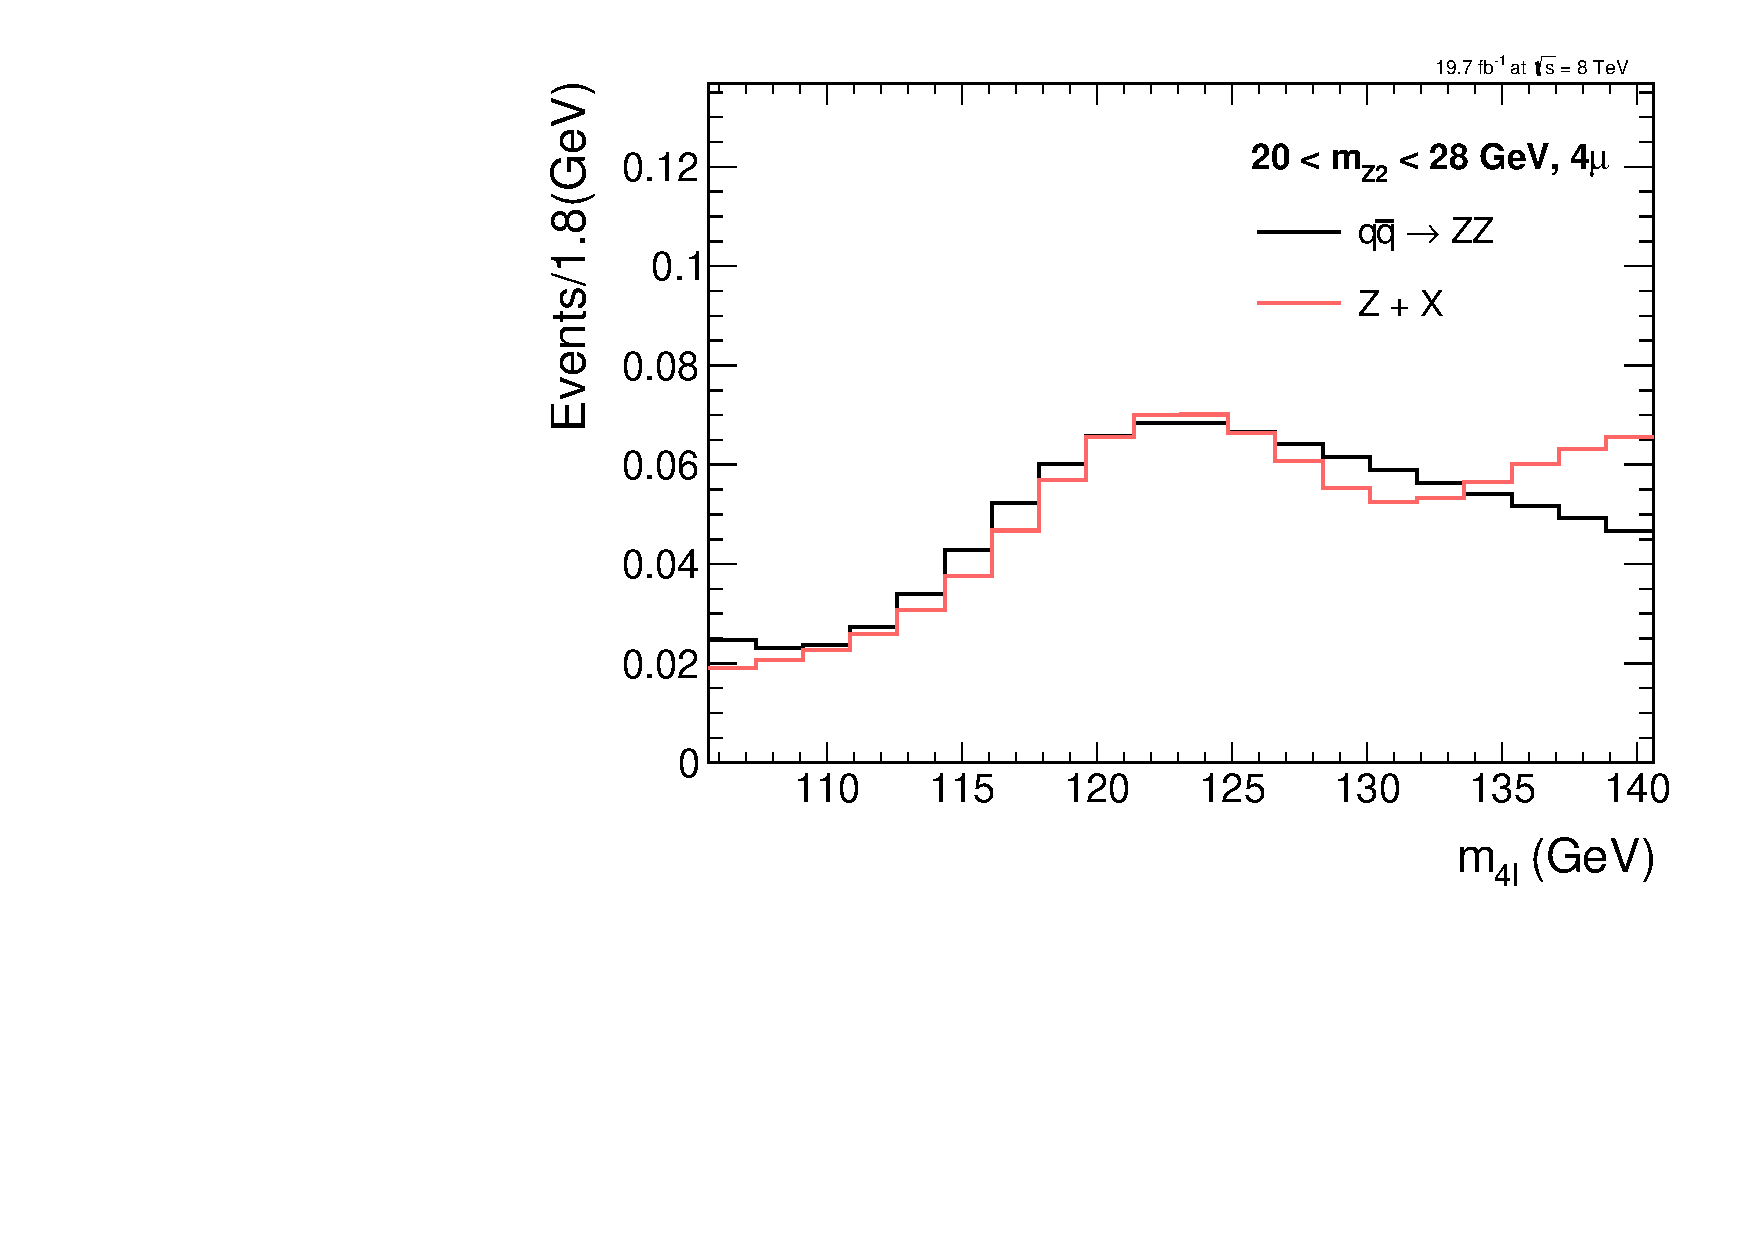
\includegraphics[width=0.30\textwidth,angle=0]{Appendix/figures/XSTemplates_4mu_massZ2_20_28_qqZZ_ZJetsCR.pdf}
      \label{fig:bkg-massZ2-qqZZ-ZX-4mu:b}
    } 
    \subfigure[$20.0 \GeV < \mathrm{m}(\mathrm{Z}_{2}) < 28.0 \GeV$]{
      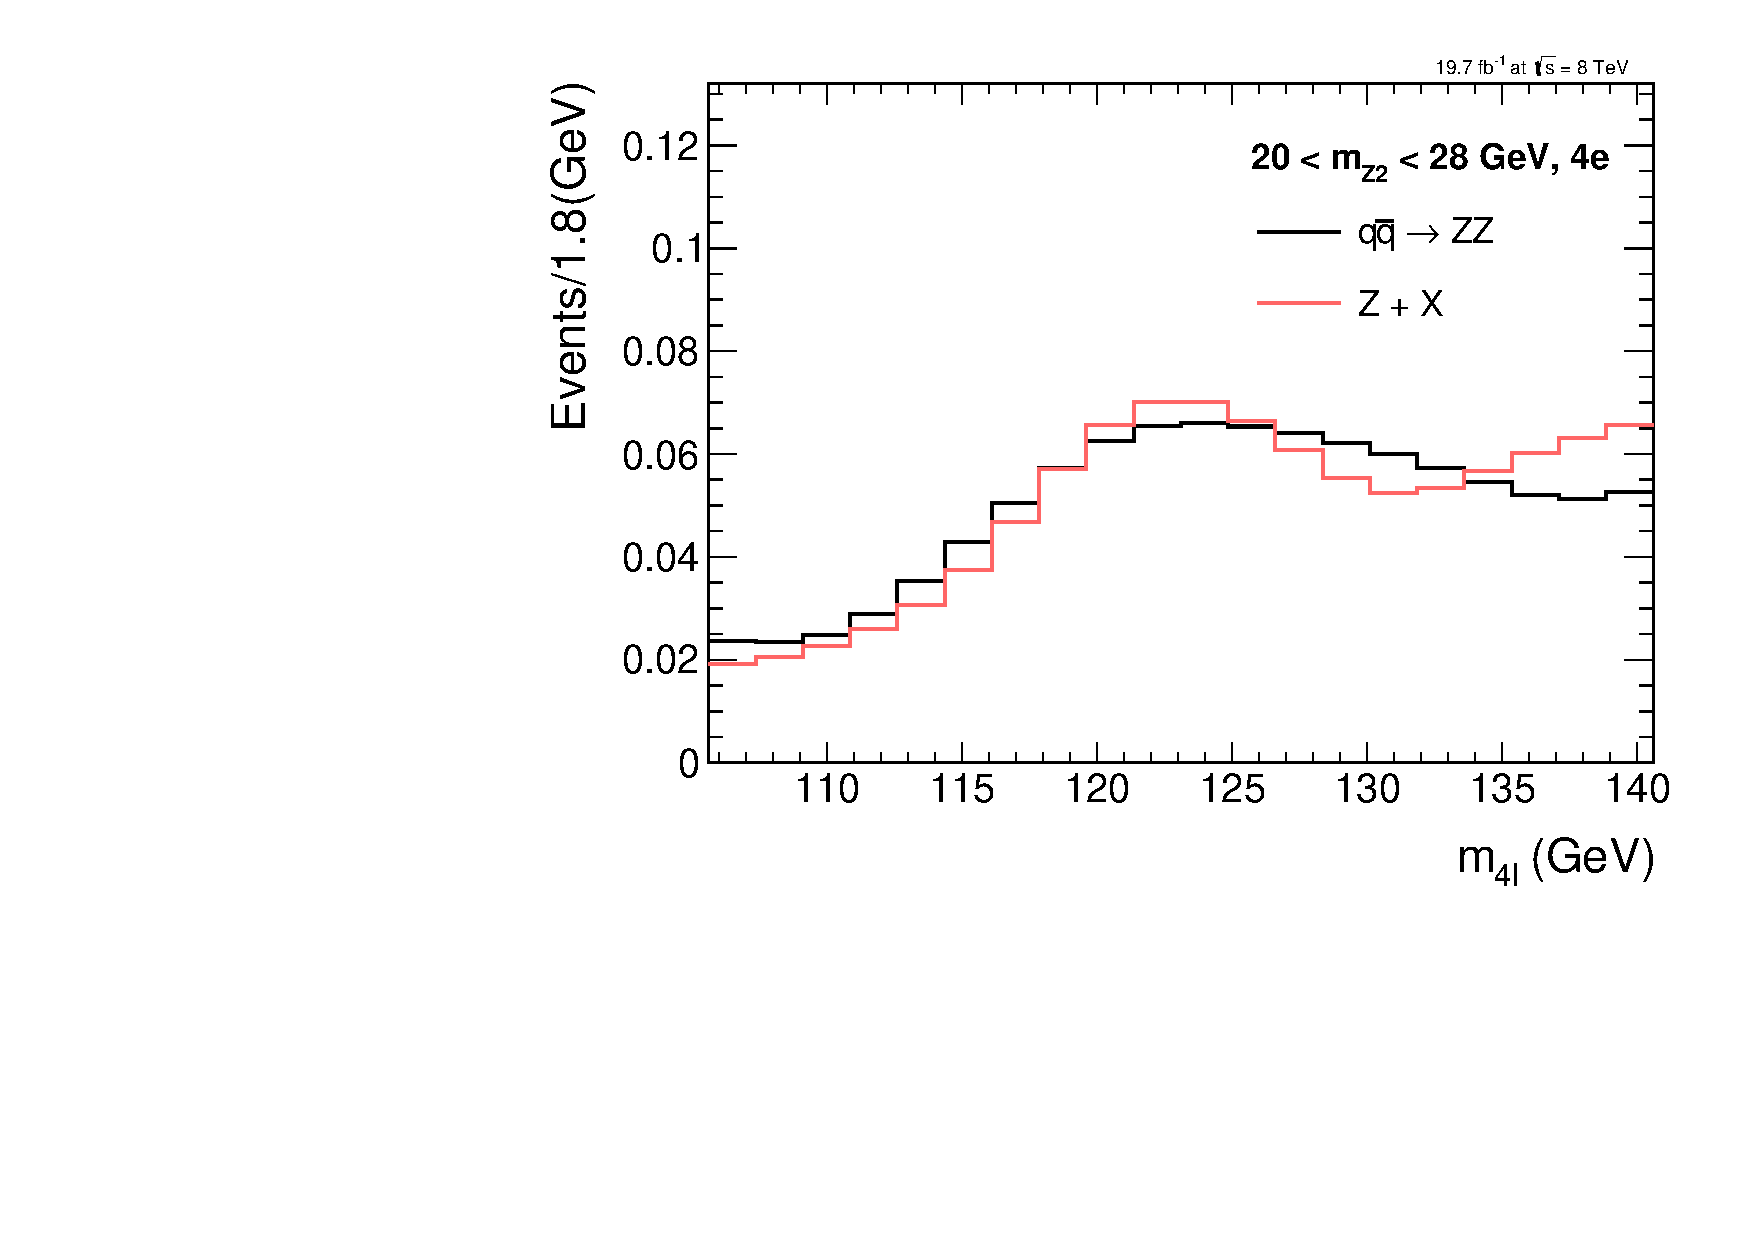
\includegraphics[width=0.30\textwidth,angle=0]{Appendix/figures/XSTemplates_4e_massZ2_20_28_qqZZ_ZJetsCR.pdf}
      \label{fig:bkg-massZ2-qqZZ-ZX-4e:b}
    } \\
    
    \subfigure[$28.0 \GeV < \mathrm{m}(\mathrm{Z}_{2}) < 35.0 \GeV$]{
      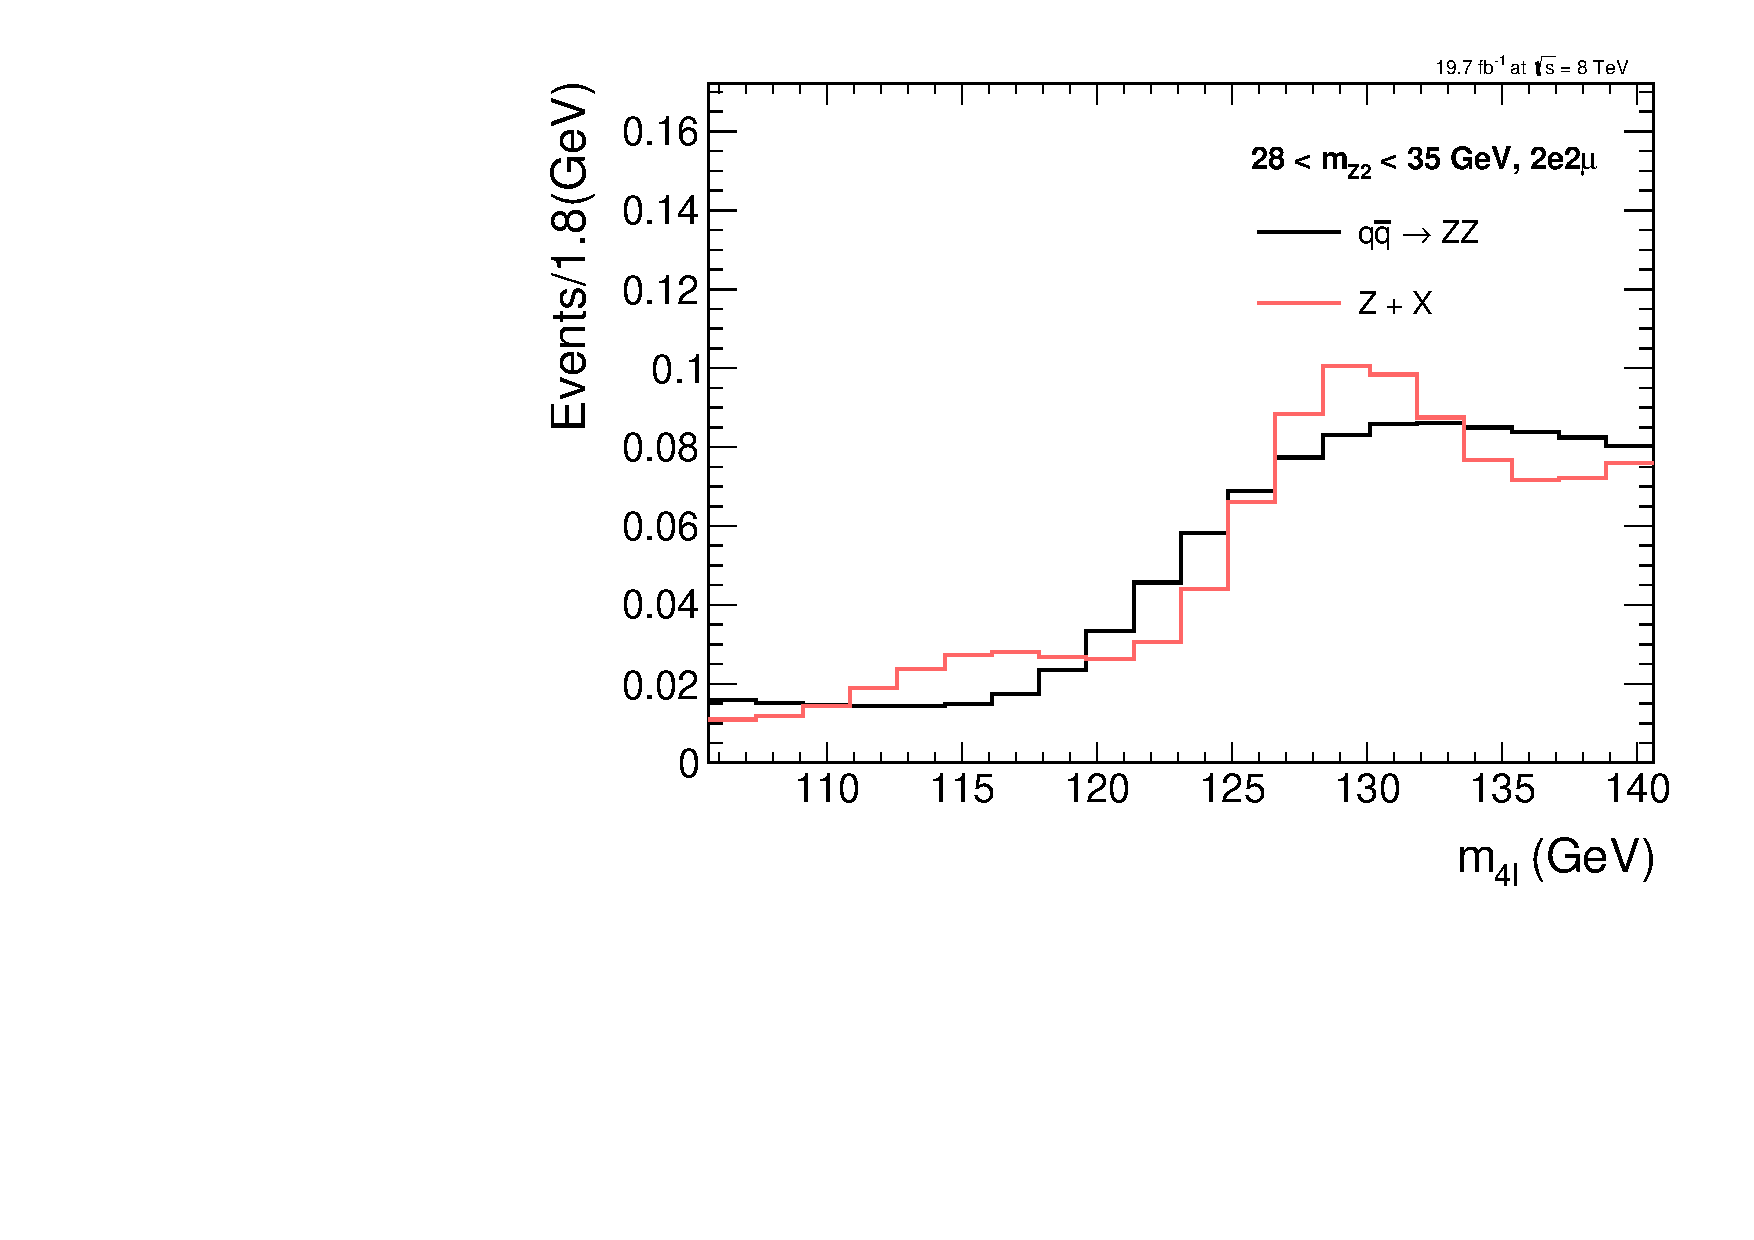
\includegraphics[width=0.30\textwidth,angle=0]{Appendix/figures/XSTemplates_2e2mu_massZ2_28_35_qqZZ_ZJetsCR.pdf}
      \label{fig:bkg-massZ2-qqZZ-ZX-2e2mu:c}
    }
    \subfigure[$28.0 \GeV < \mathrm{m}(\mathrm{Z}_{2}) < 35.0 \GeV$]{
      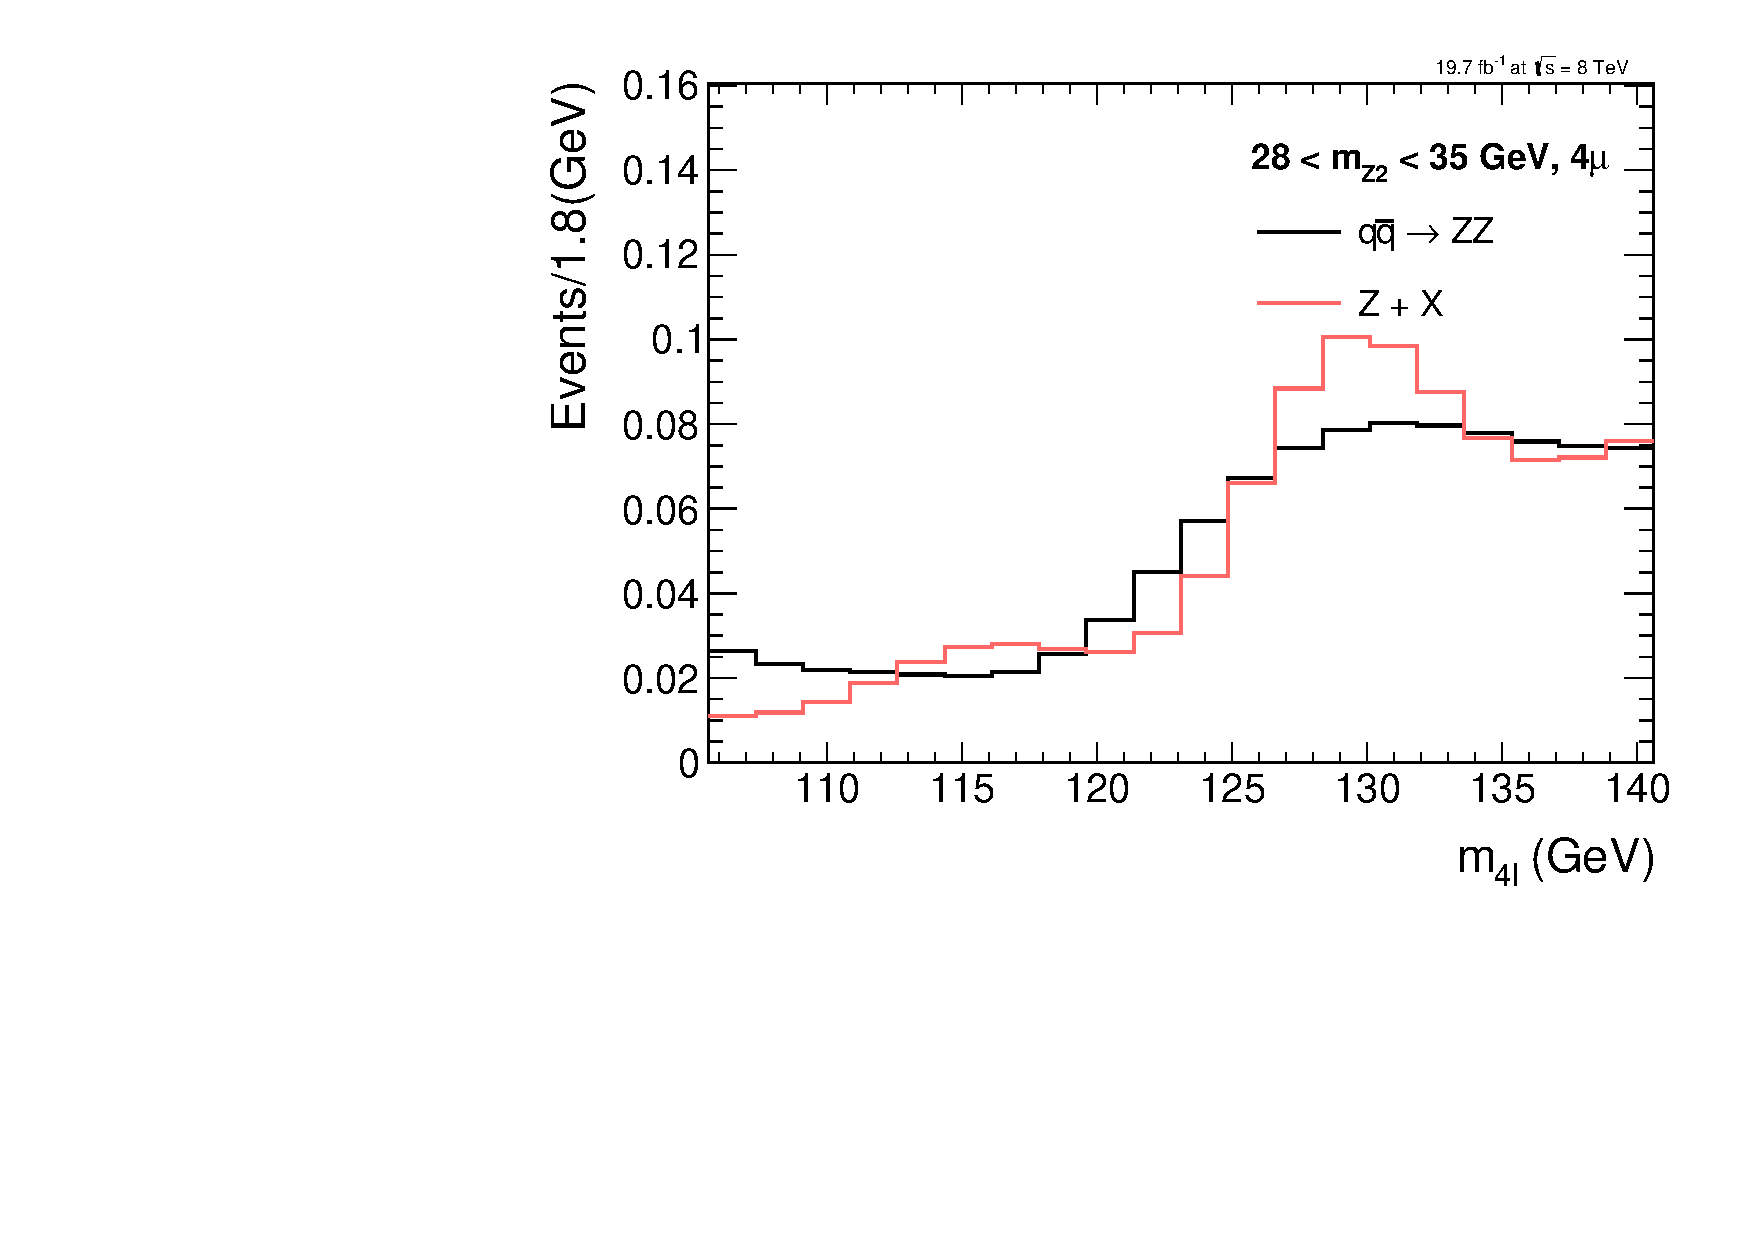
\includegraphics[width=0.30\textwidth,angle=0]{Appendix/figures/XSTemplates_4mu_massZ2_28_35_qqZZ_ZJetsCR.pdf}
      \label{fig:bkg-massZ2-qqZZ-ZX-4mu:c}
    }
    \subfigure[$28.0 \GeV < \mathrm{m}(\mathrm{Z}_{2}) < 35.0 \GeV$]{
      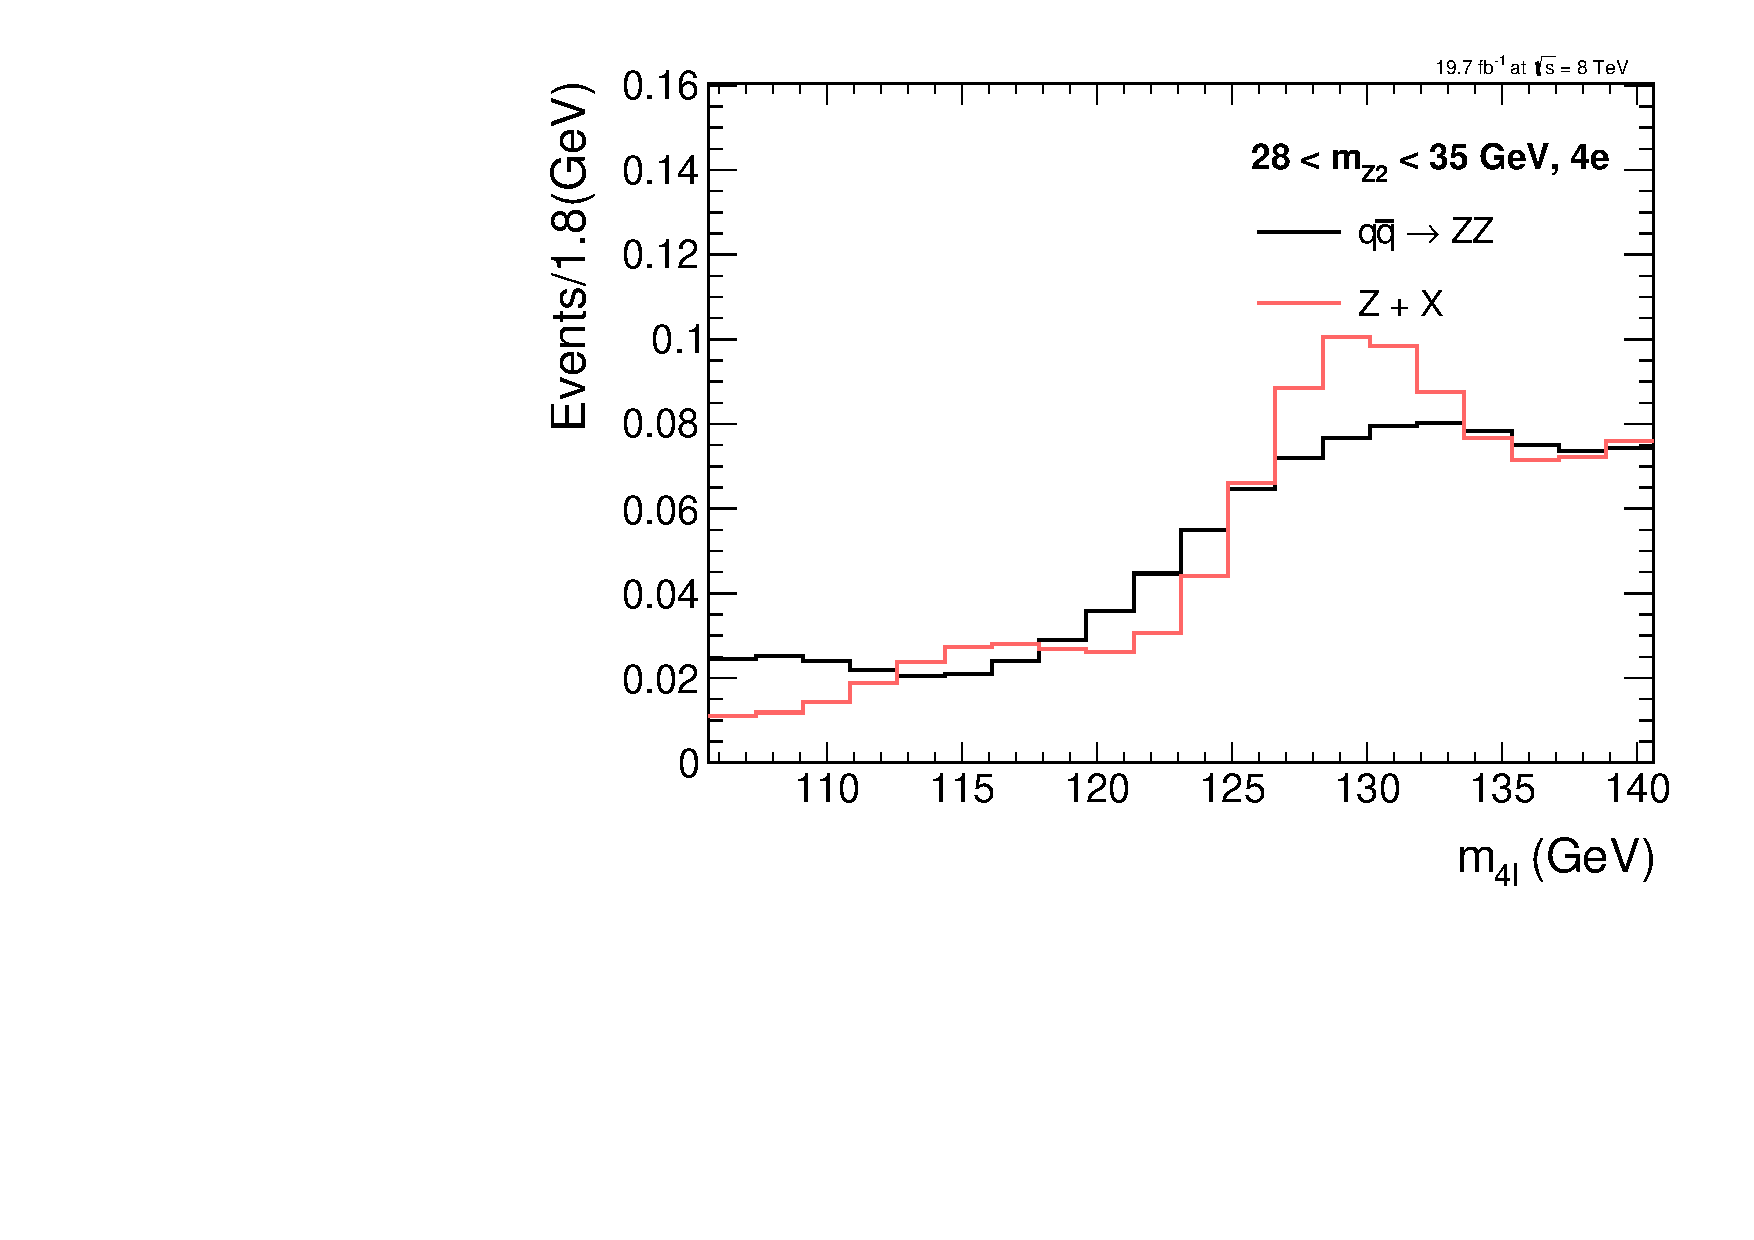
\includegraphics[width=0.30\textwidth,angle=0]{Appendix/figures/XSTemplates_4e_massZ2_28_35_qqZZ_ZJetsCR.pdf}
      \label{fig:bkg-massZ2-qqZZ-ZX-4e:c}
    } \\
    
    \subfigure[$35.0 \GeV < \mathrm{m}(\mathrm{Z}_{2}) < 120.0 \GeV$]{
      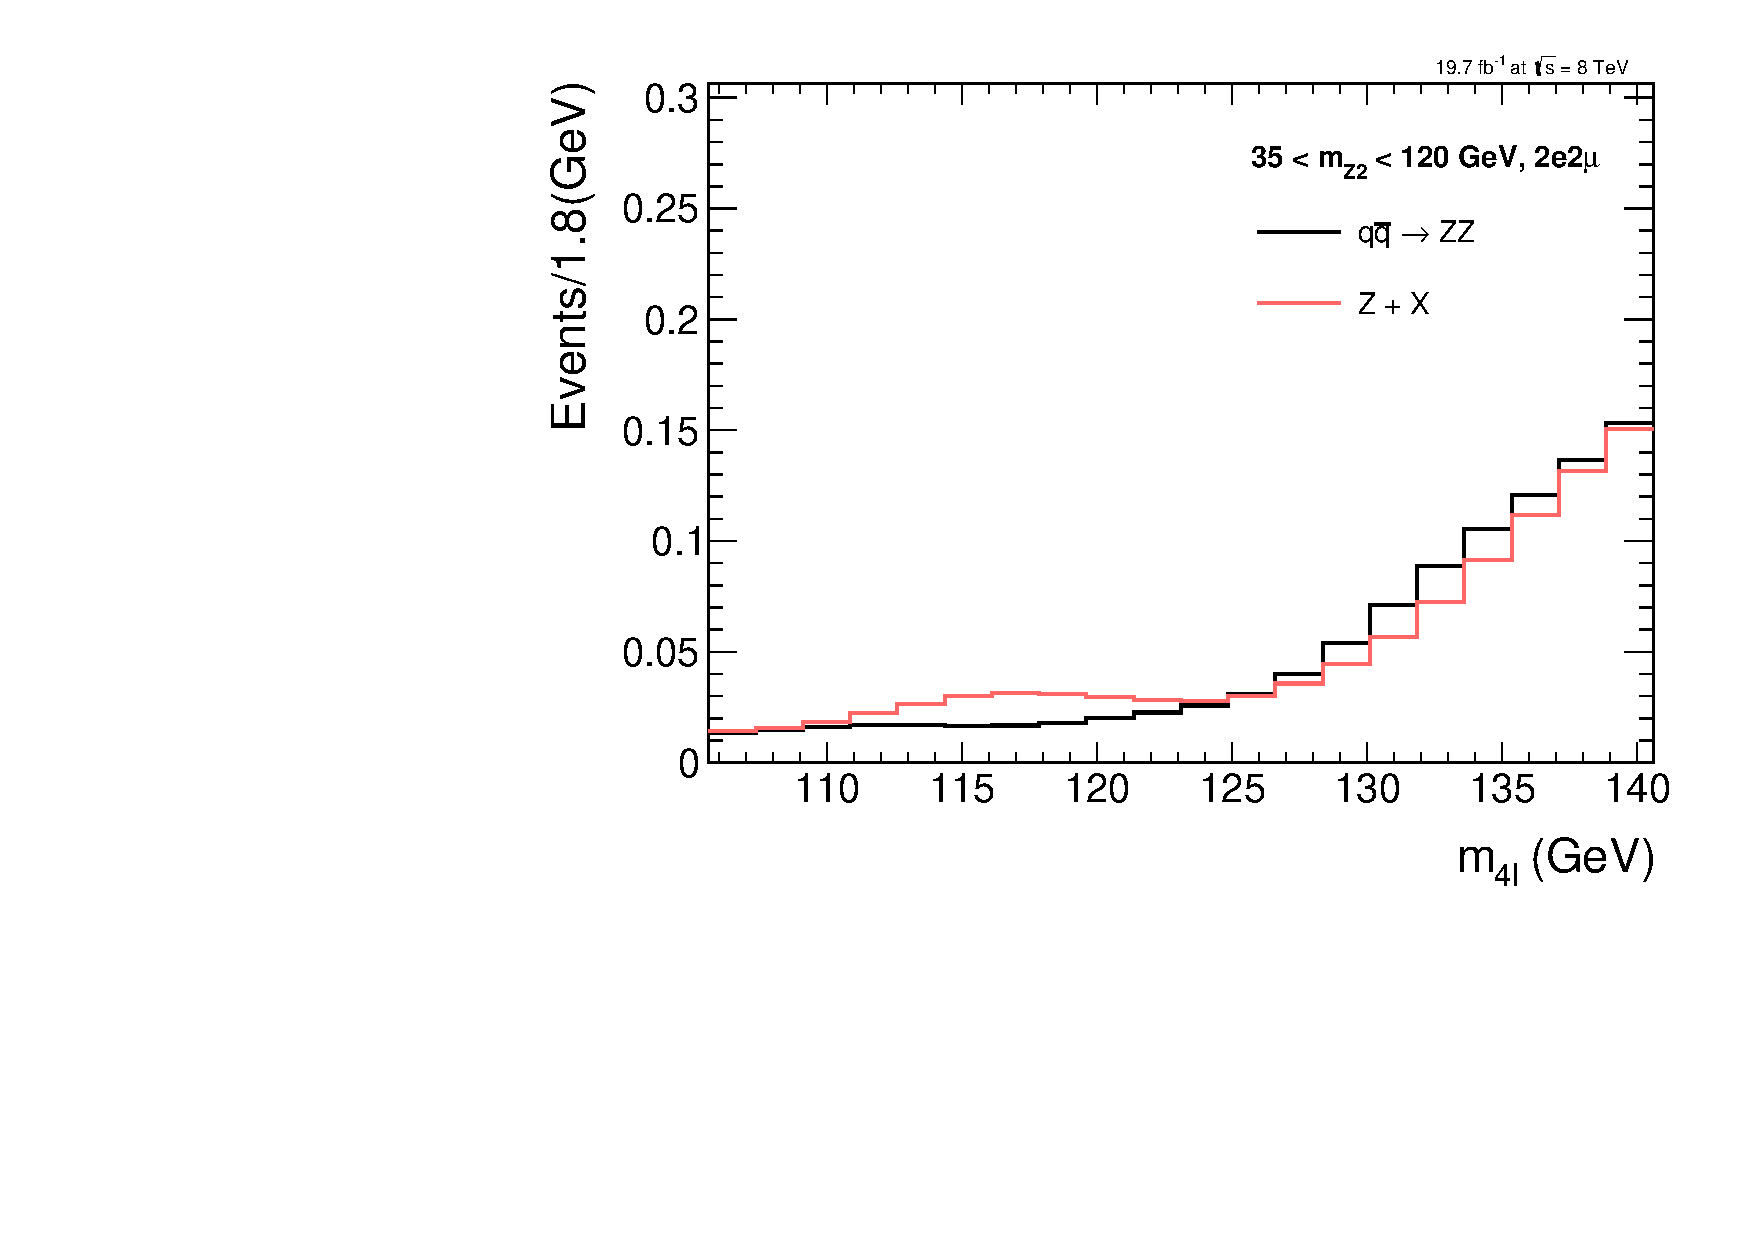
\includegraphics[width=0.30\textwidth,angle=0]{Appendix/figures/XSTemplates_2e2mu_massZ2_35_120_qqZZ_ZJetsCR.pdf}
      \label{fig:bkg-massZ2-qqZZ-ZX-2e2mu:d}
    }
    \subfigure[$35.0 \GeV < \mathrm{m}(\mathrm{Z}_{2}) < 120.0 \GeV$]{
      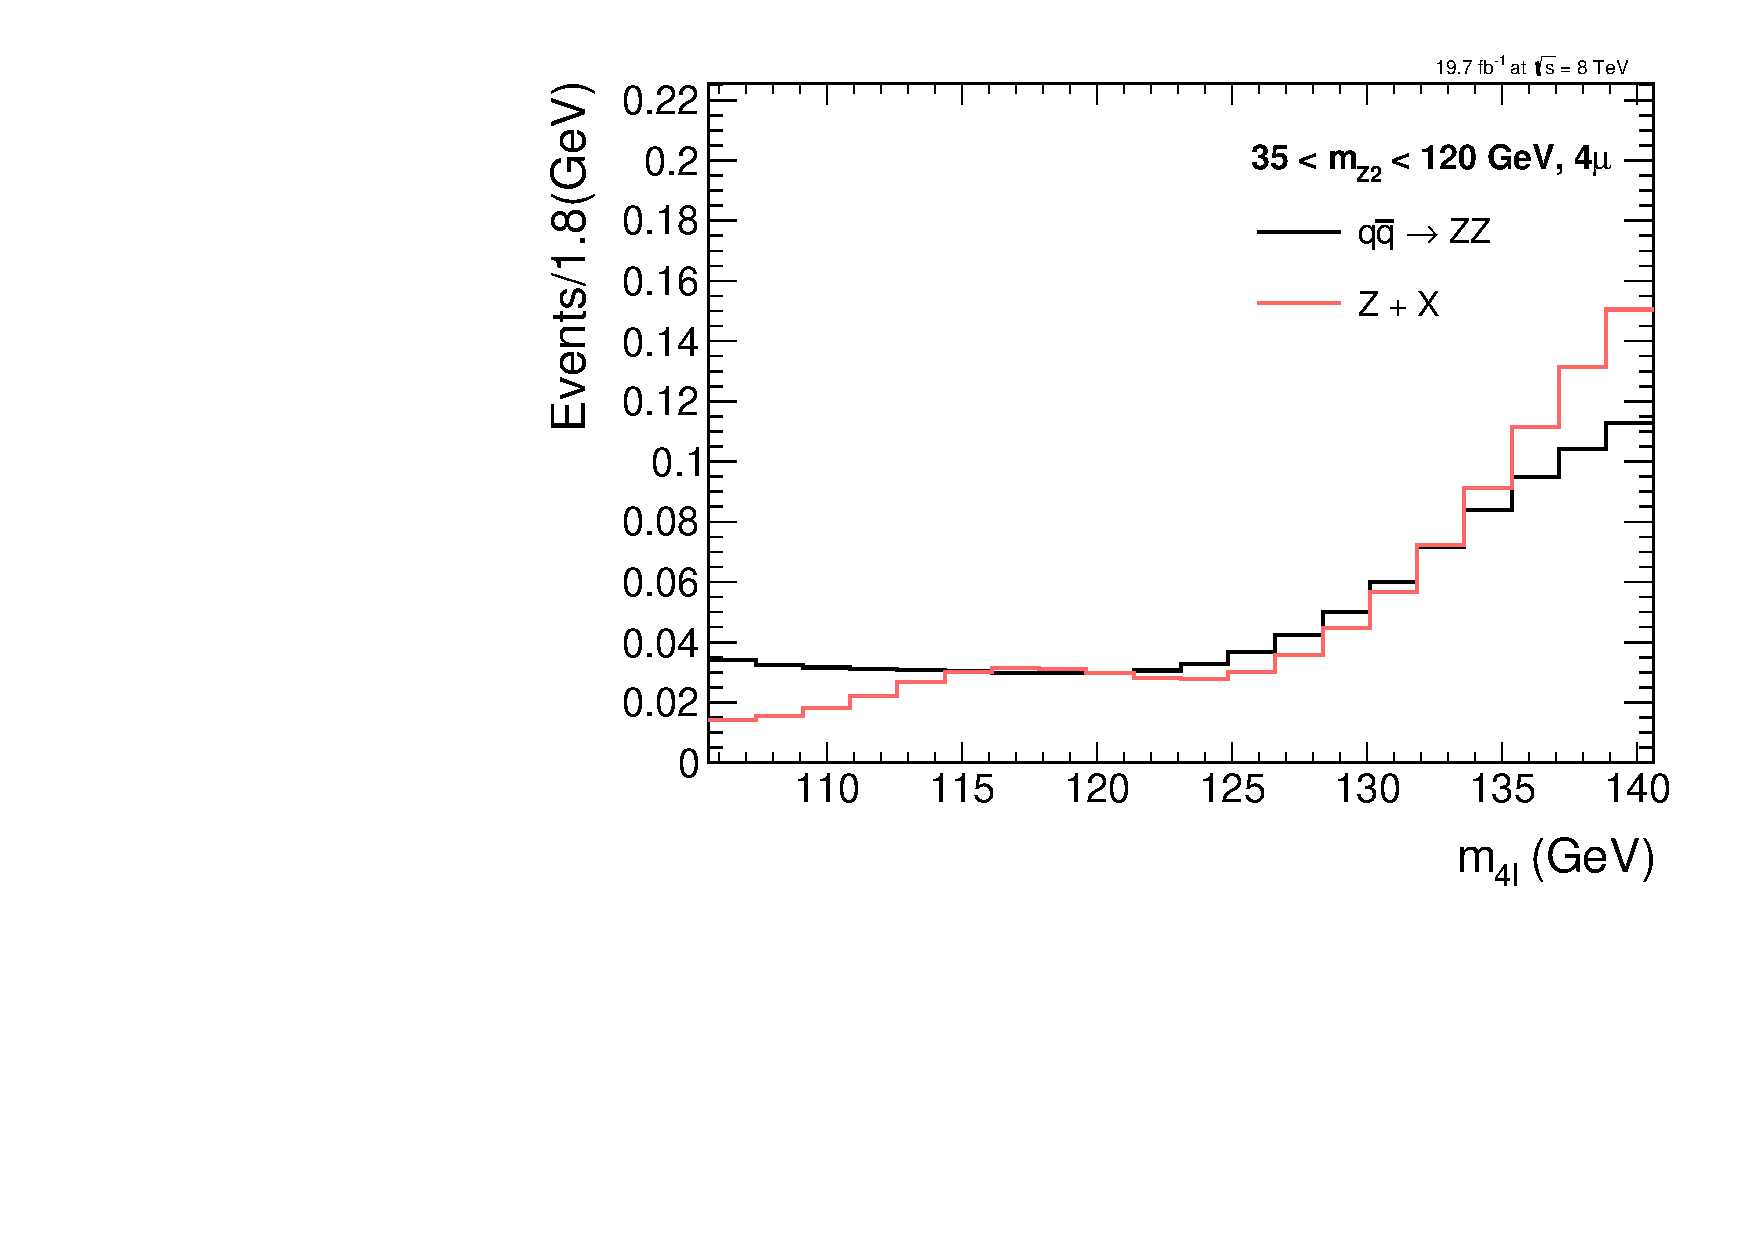
\includegraphics[width=0.30\textwidth,angle=0]{Appendix/figures/XSTemplates_4mu_massZ2_35_120_qqZZ_ZJetsCR.pdf}
      \label{fig:bkg-massZ2-qqZZ-ZX-4mu:d}
    }
    \subfigure[$35.0 \GeV < \mathrm{m}(\mathrm{Z}_{2}) < 120.0 \GeV$]{
      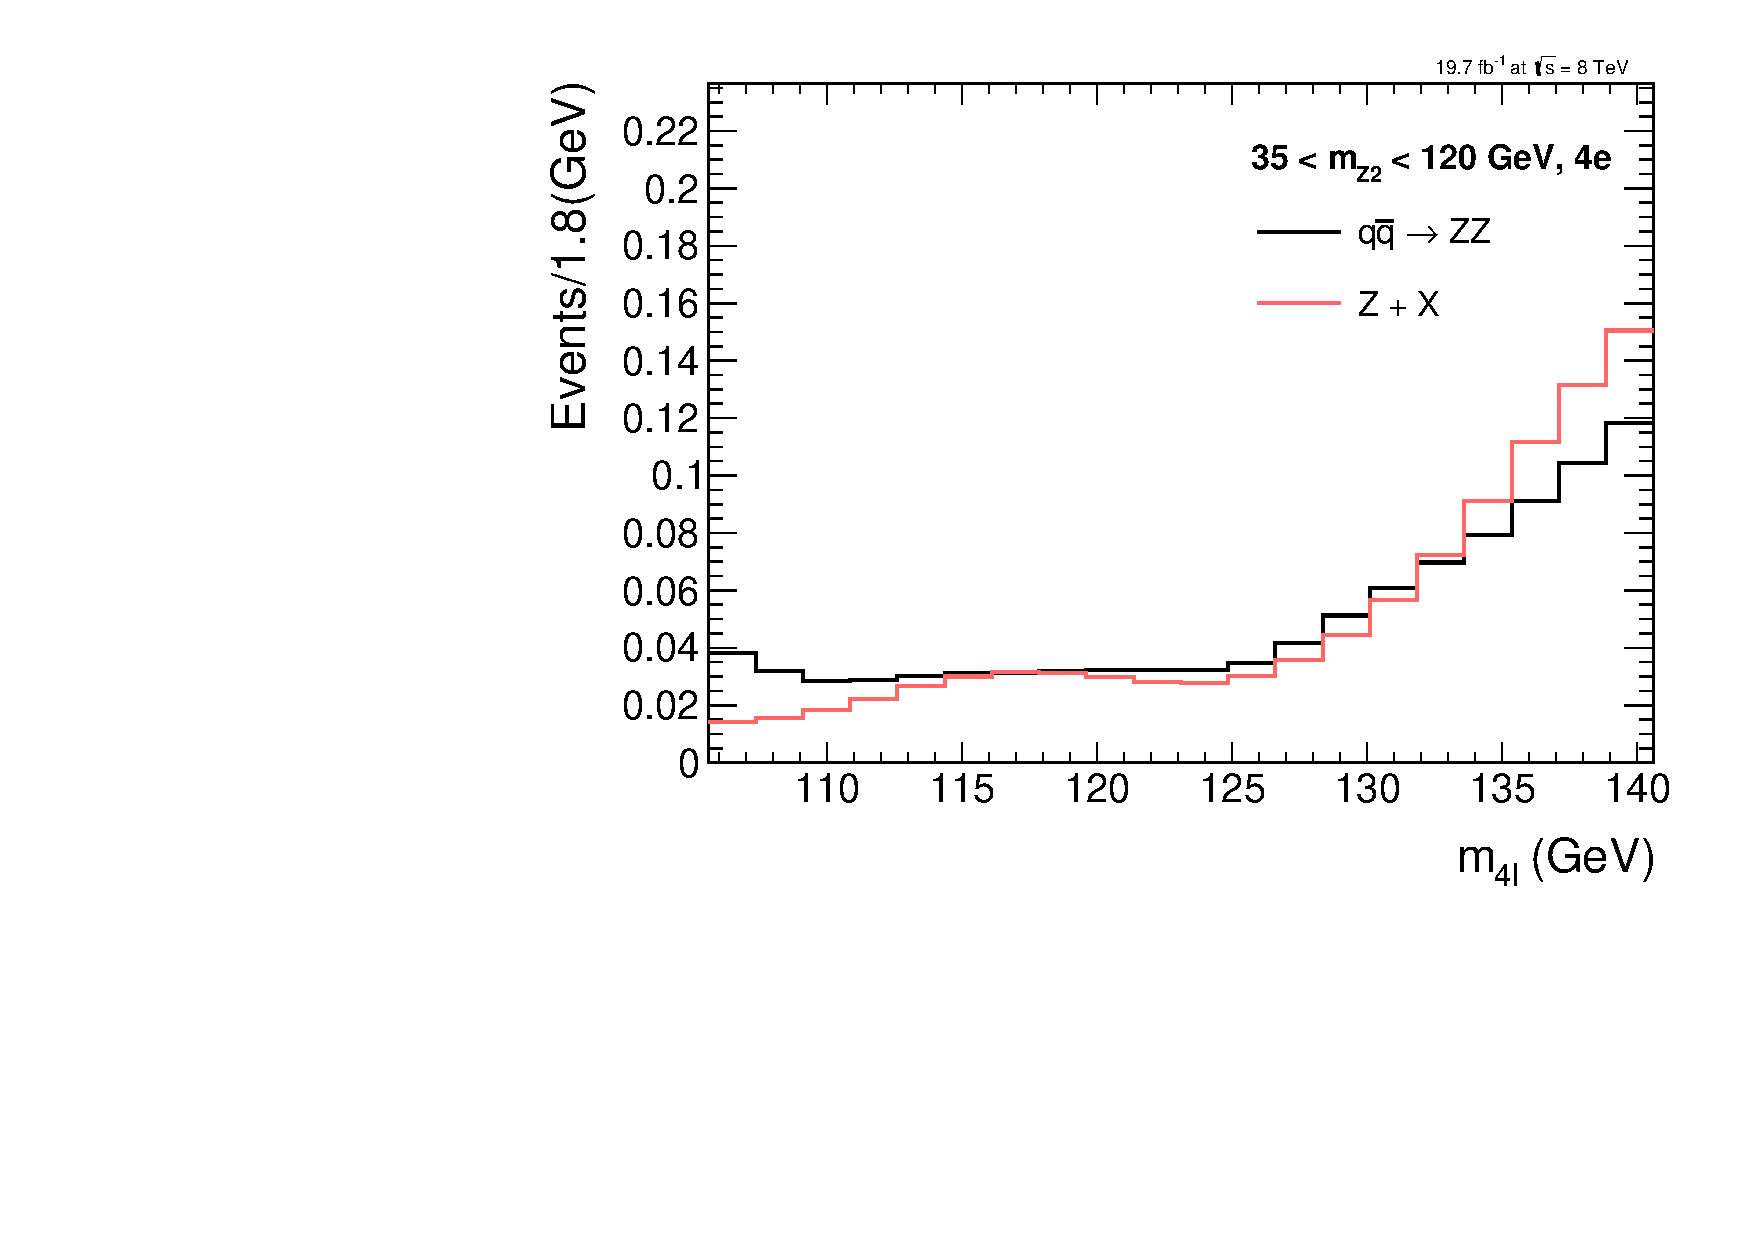
\includegraphics[width=0.30\textwidth,angle=0]{Appendix/figures/XSTemplates_4e_massZ2_35_120_qqZZ_ZJetsCR.pdf}
      \label{fig:bkg-massZ2-qqZZ-ZX-4e:d}
    } \\
    
    \caption{ Distributions of m($4\ell$) for the $qq \rightarrow \mathrm{ZZ}$ and Z+X backgrounds in different bins of $m(\mathrm{Z}_{2})$ 
    for three final states: $2e2\mu$(left), $4\mu$(middle) and $4e$(right).}
  \label{fig:bkg-massZ2-qqZZ-ZX}
  
 \end{center}
\end{figure} 

 \clearpage
 
 \begin{figure}[!ht]
  \begin{center}
  
    \subfigure[$12.0 \GeV < \mathrm{m}(\mathrm{Z}_{2}) < 20.0 \GeV$]{
      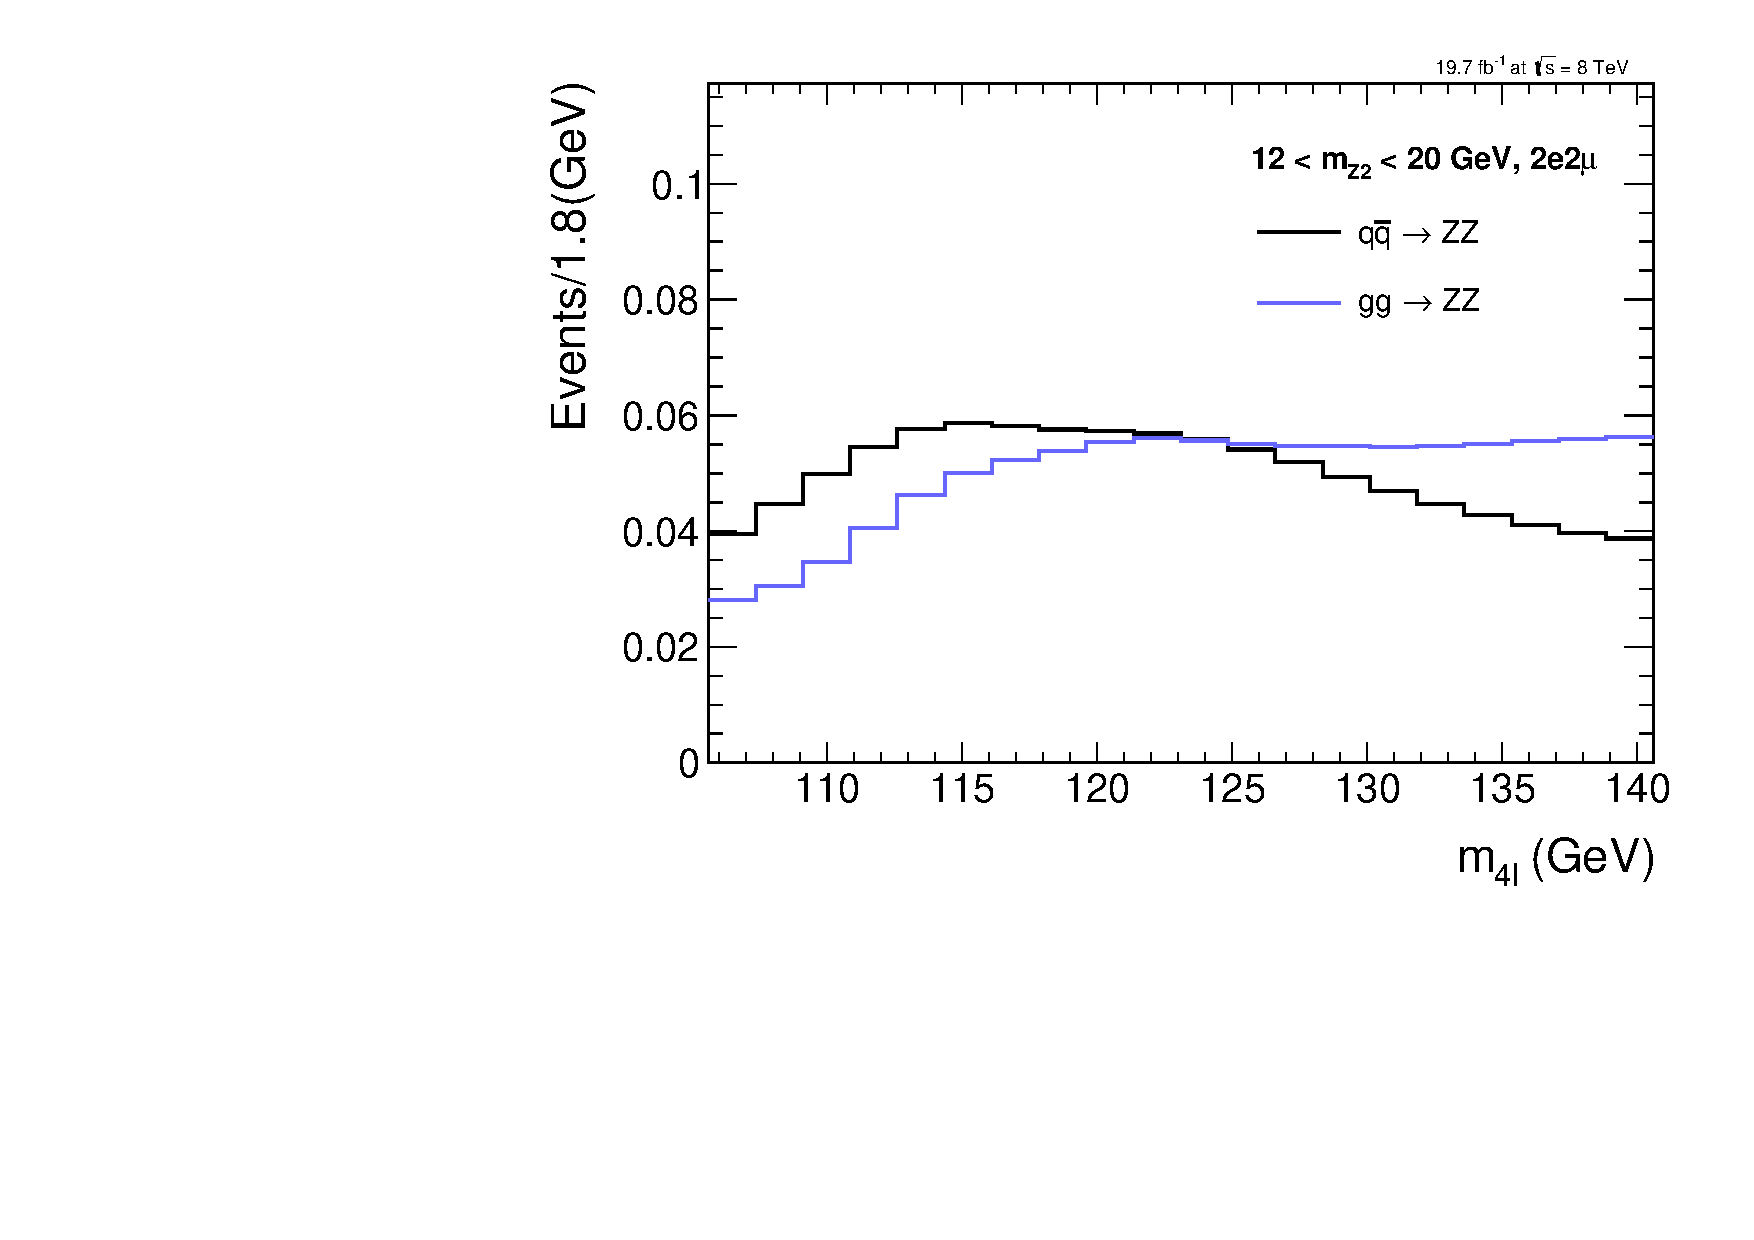
\includegraphics[width=0.30\textwidth,angle=0]{Appendix/figures/XSTemplates_2e2mu_massZ2_12_20_qqZZ_ggZZ.pdf}
      \label{fig:bkg-massZ2-qqZZ-ggZZ-2e2mu:a}
    }    
    \subfigure[$12.0 \GeV < \mathrm{m}(\mathrm{Z}_{2}) < 20.0 \GeV$]{
      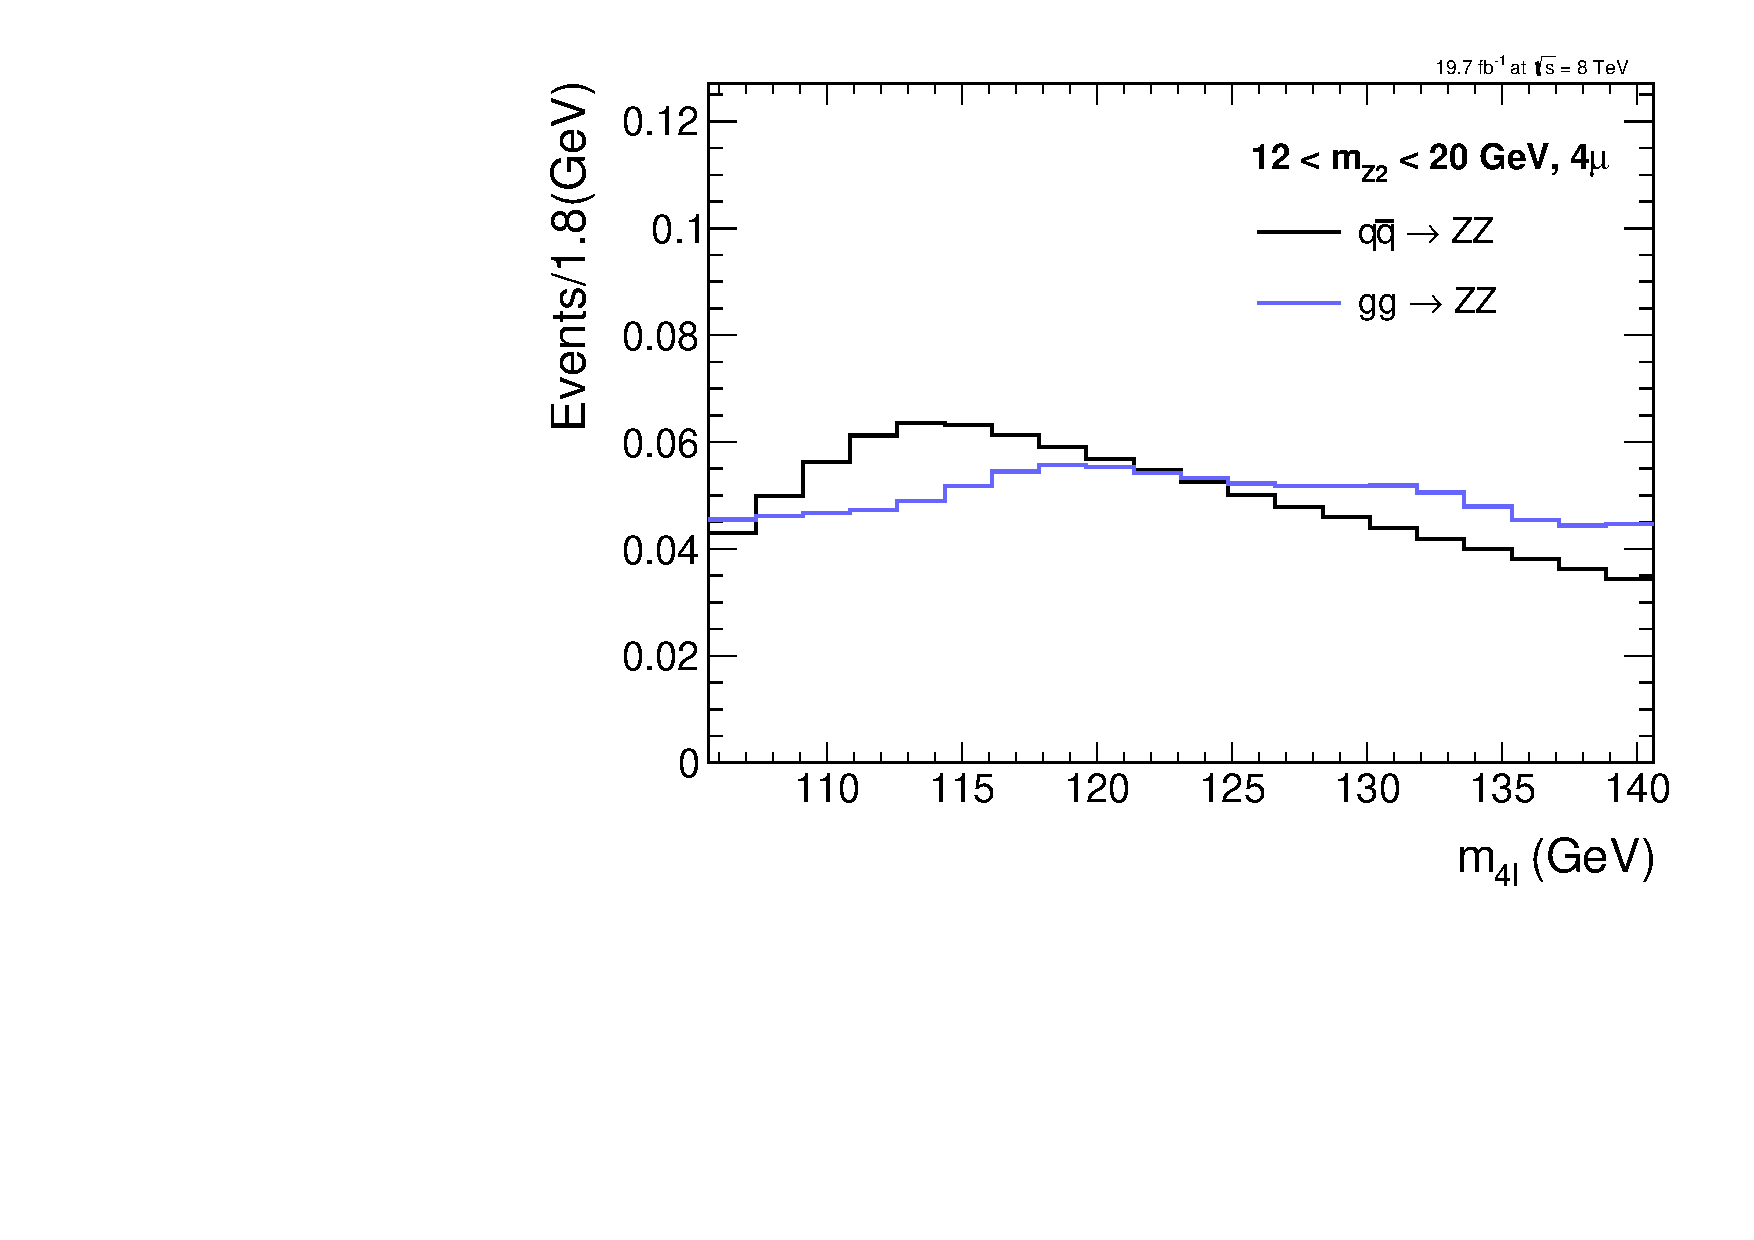
\includegraphics[width=0.30\textwidth,angle=0]{Appendix/figures/XSTemplates_4mu_massZ2_12_20_qqZZ_ggZZ.pdf}
      \label{fig:bkg-massZ2-qqZZ-ggZZ-4mu:a}
    }    
    \subfigure[$12.0 \GeV < \mathrm{m}(\mathrm{Z}_{2}) < 20.0 \GeV$]{
      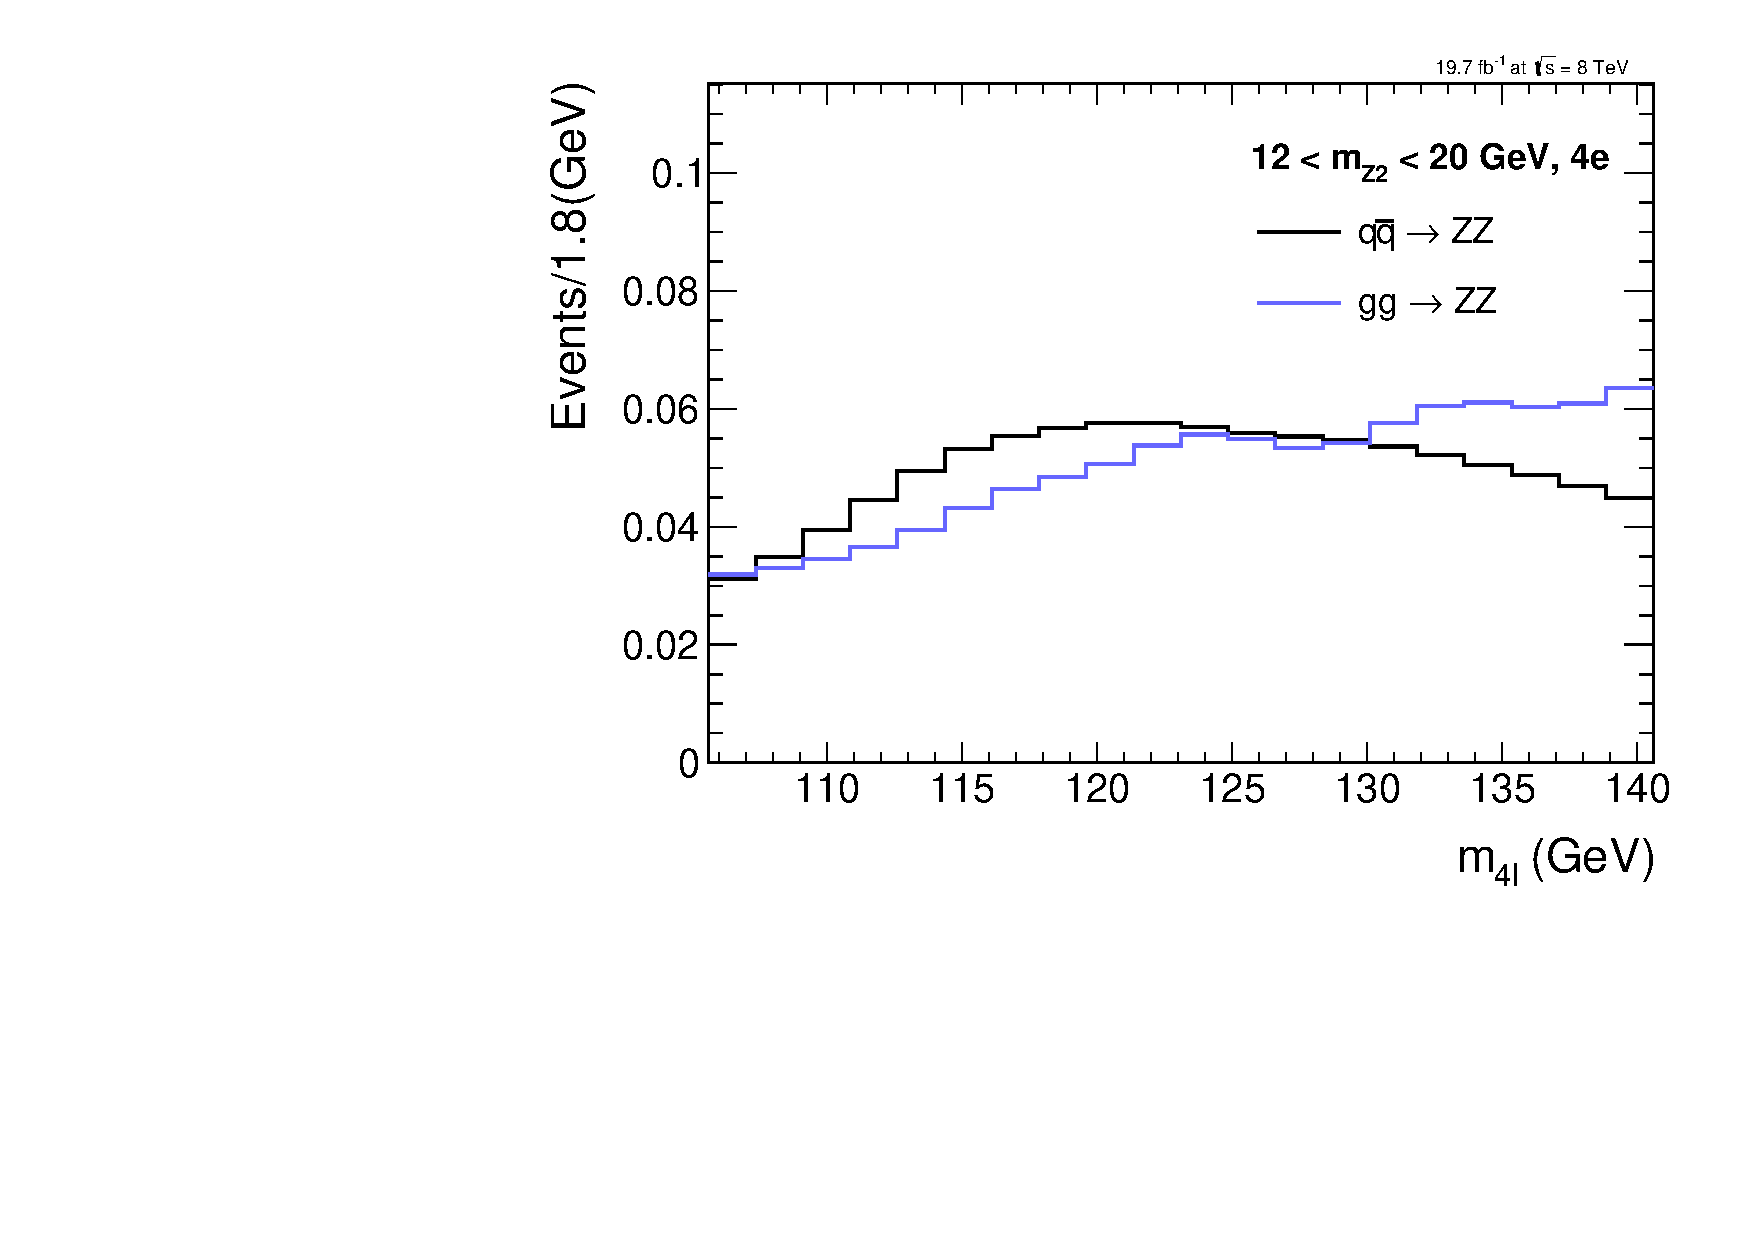
\includegraphics[width=0.30\textwidth,angle=0]{Appendix/figures/XSTemplates_4e_massZ2_12_20_qqZZ_ggZZ.pdf}
      \label{fig:bkg-massZ2-qqZZ-ggZZ-4e:a}
    }    \\

    \subfigure[$20.0 \GeV < \mathrm{m}(\mathrm{Z}_{2}) < 28.0 \GeV$]{
      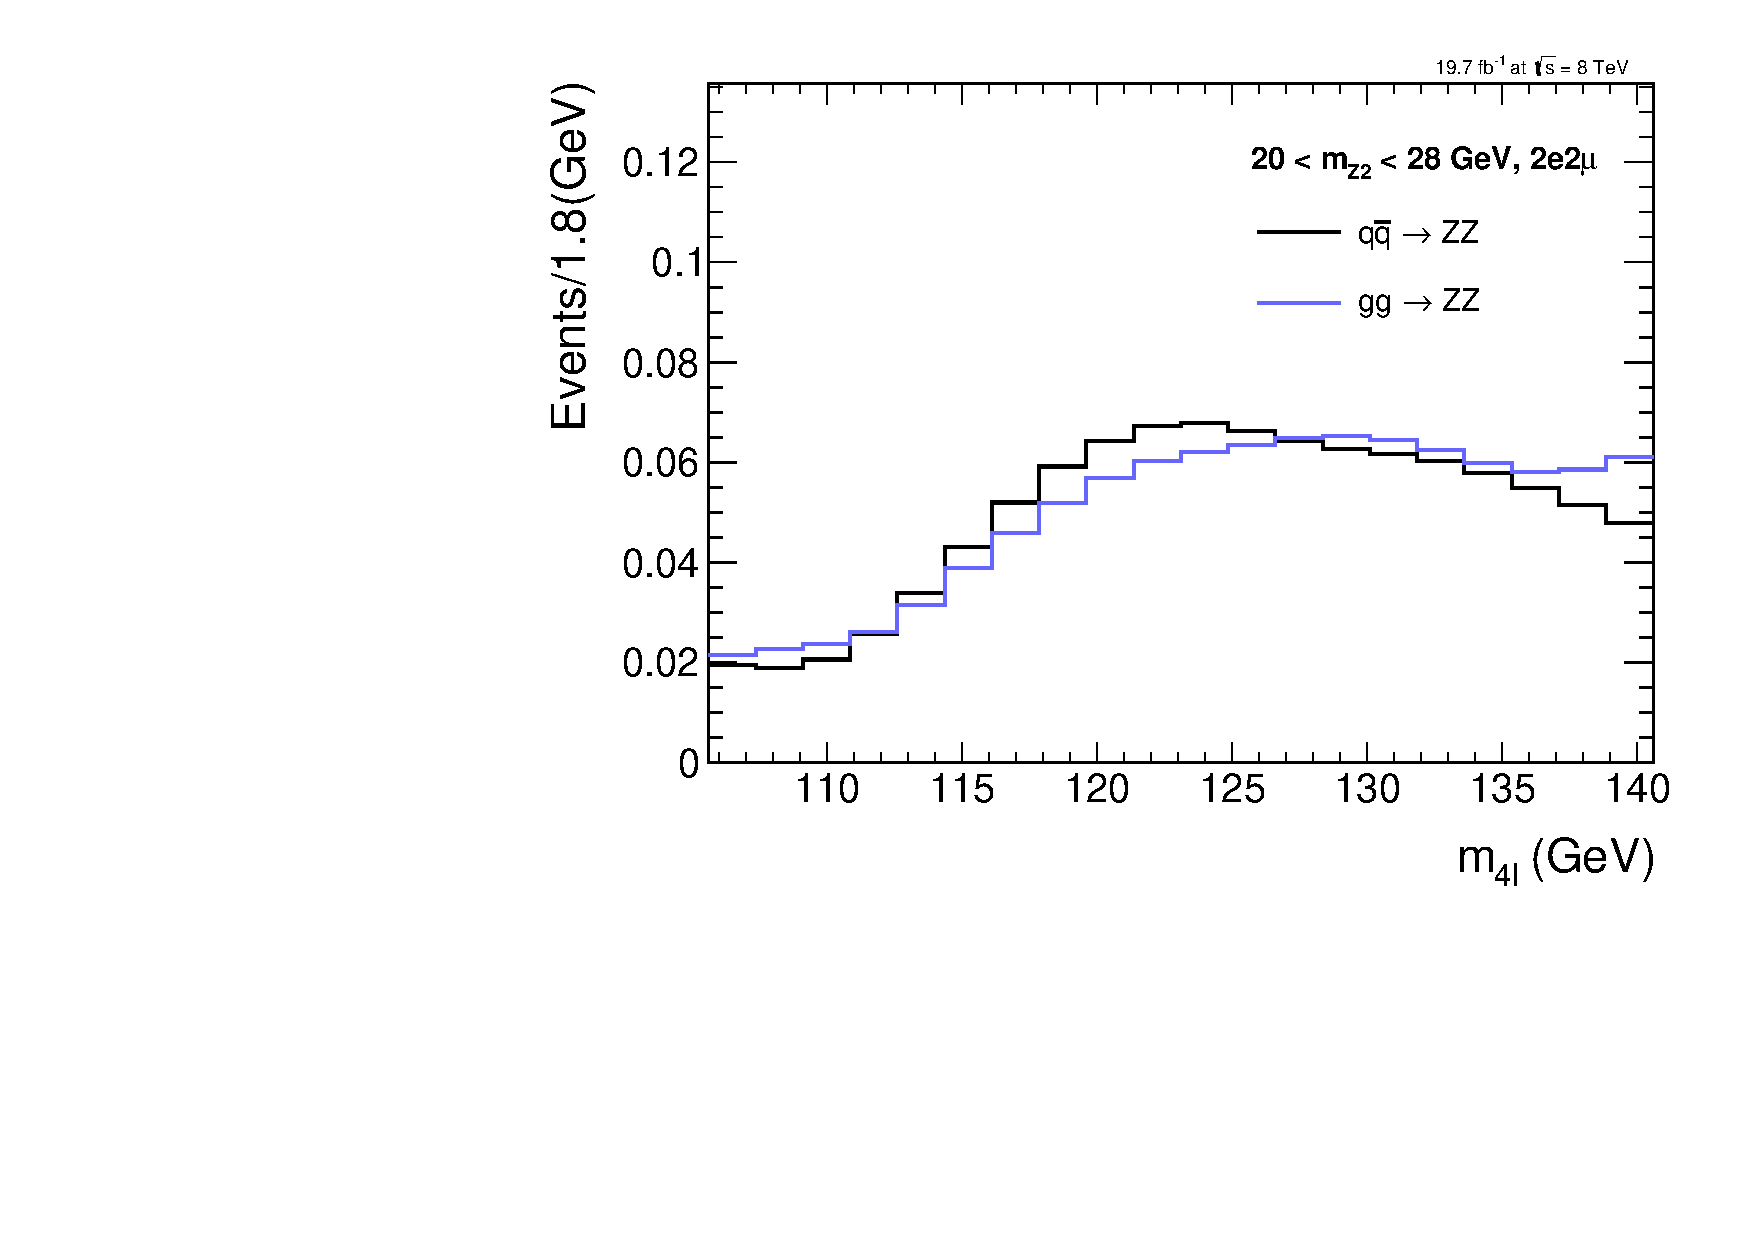
\includegraphics[width=0.30\textwidth,angle=0]{Appendix/figures/XSTemplates_2e2mu_massZ2_20_28_qqZZ_ggZZ.pdf}
      \label{fig:bkg-massZ2-qqZZ-ggZZ-2e2mu:b}
    }
    \subfigure[$20.0 \GeV < \mathrm{m}(\mathrm{Z}_{2}) < 28.0 \GeV$]{
      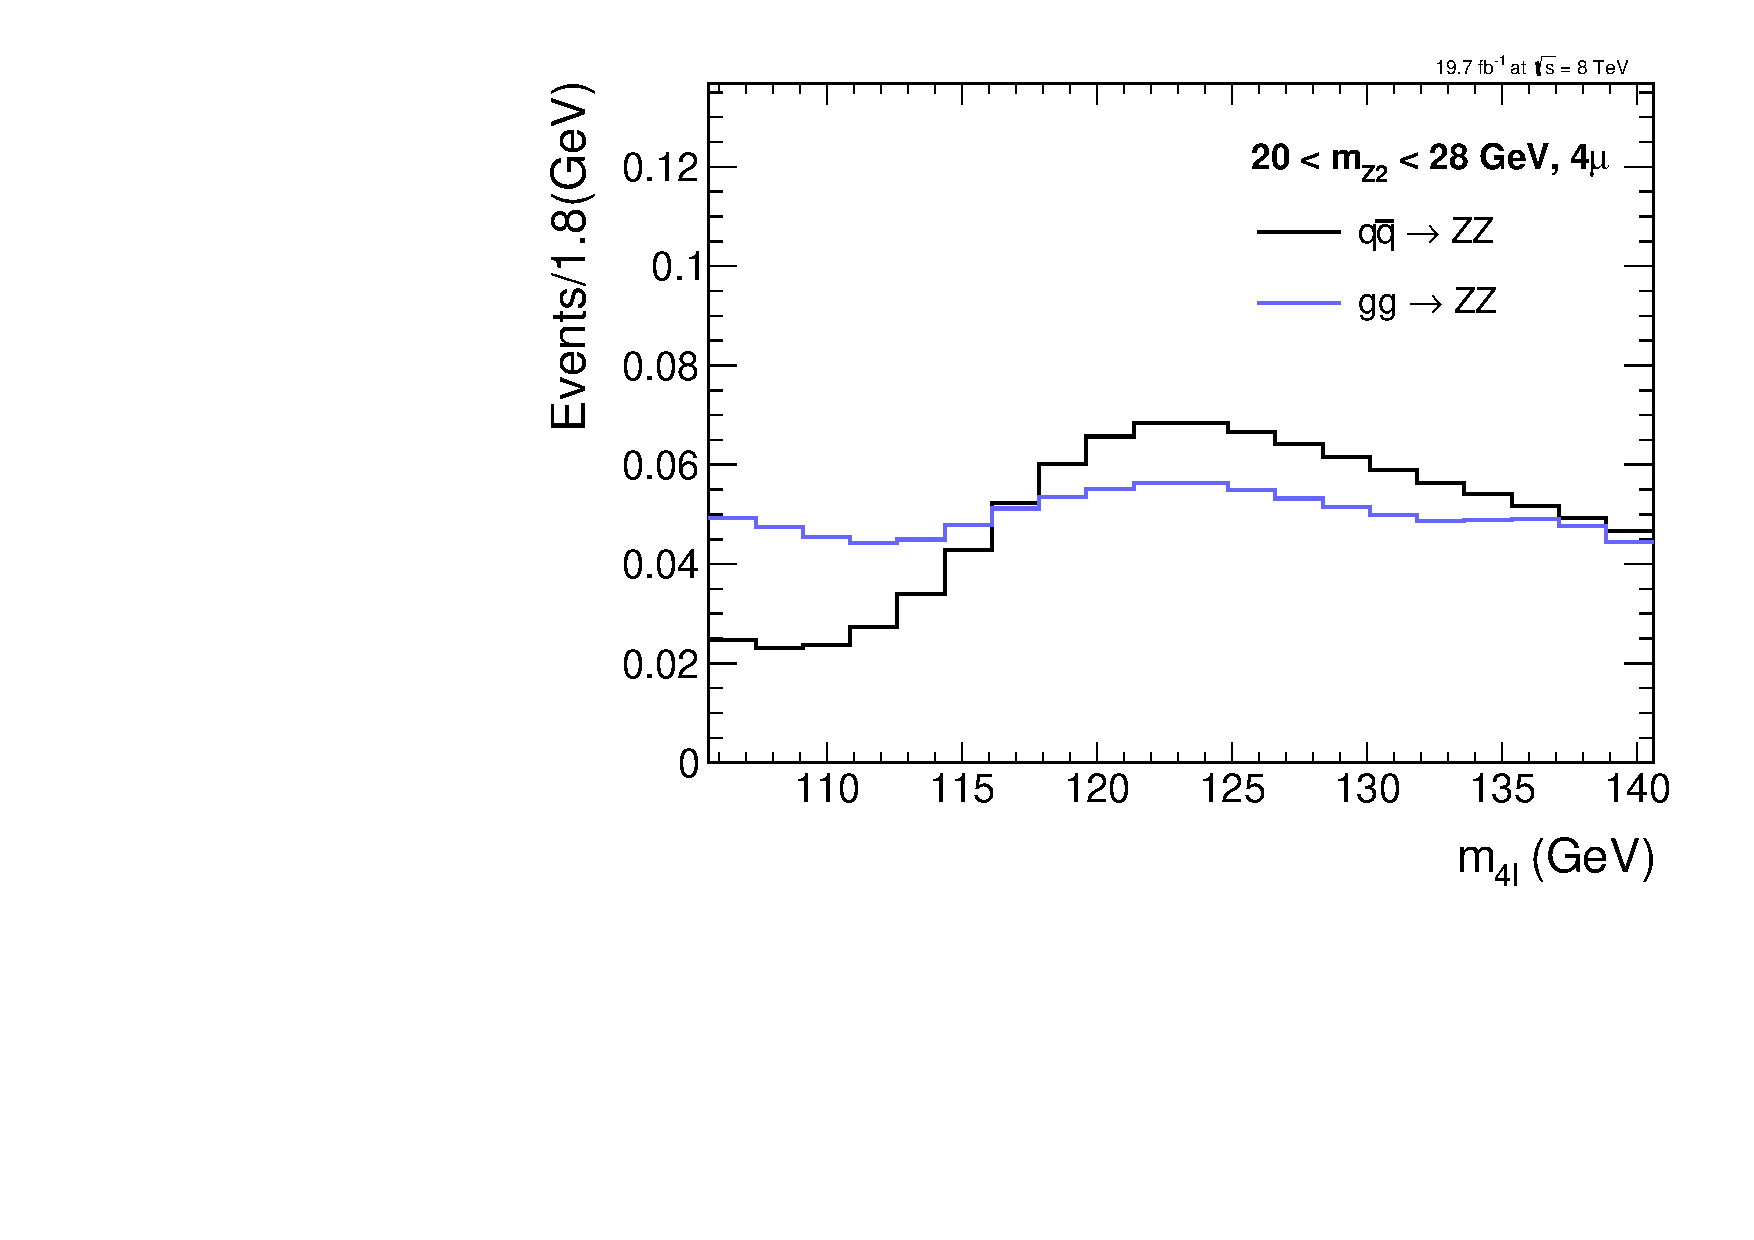
\includegraphics[width=0.30\textwidth,angle=0]{Appendix/figures/XSTemplates_4mu_massZ2_20_28_qqZZ_ggZZ.pdf}
      \label{fig:bkg-massZ2-qqZZ-ggZZ-4mu:b}
    } 
    \subfigure[$20.0 \GeV < \mathrm{m}(\mathrm{Z}_{2}) < 28.0 \GeV$]{
      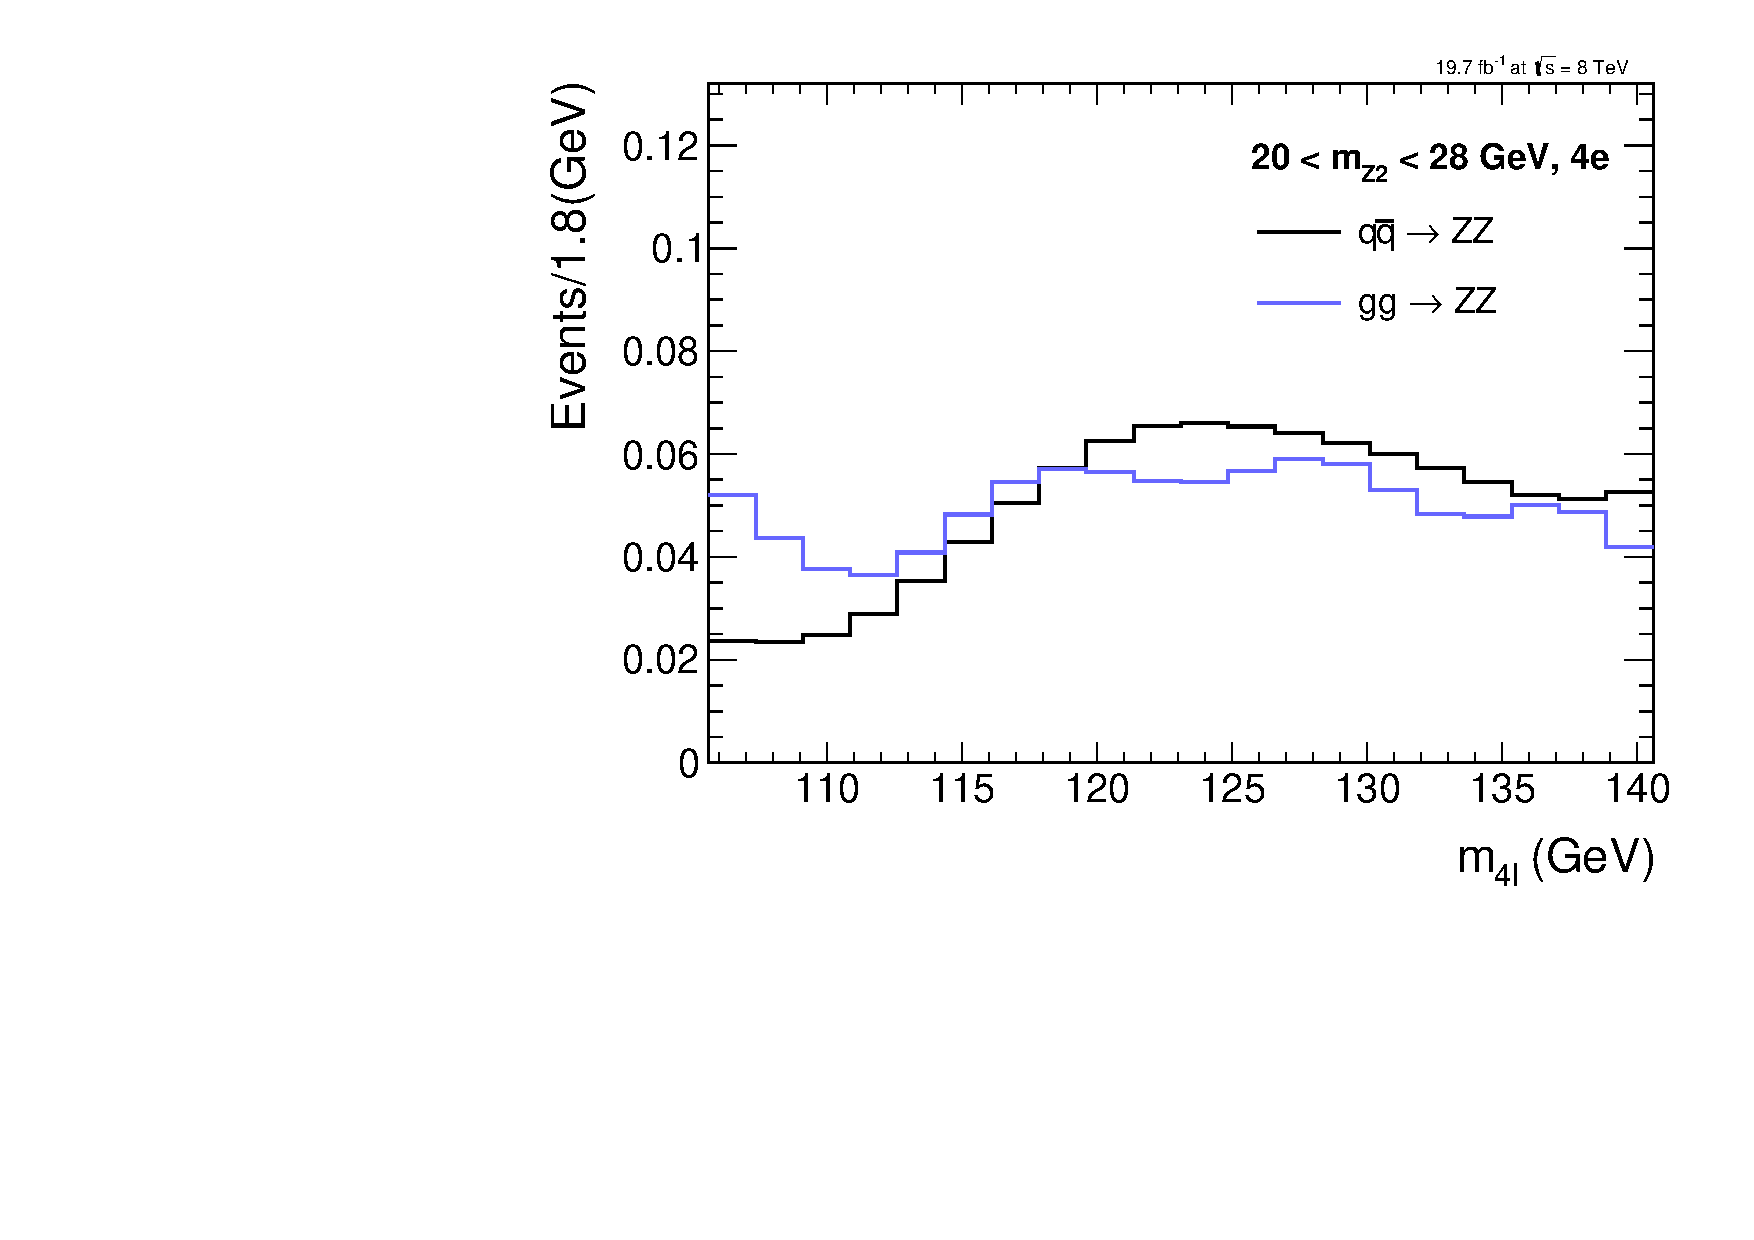
\includegraphics[width=0.30\textwidth,angle=0]{Appendix/figures/XSTemplates_4e_massZ2_20_28_qqZZ_ggZZ.pdf}
      \label{fig:bkg-massZ2-qqZZ-ggZZ-4e:b}
    } \\
    
    \subfigure[$28.0 \GeV < \mathrm{m}(\mathrm{Z}_{2}) < 35.0 \GeV$]{
      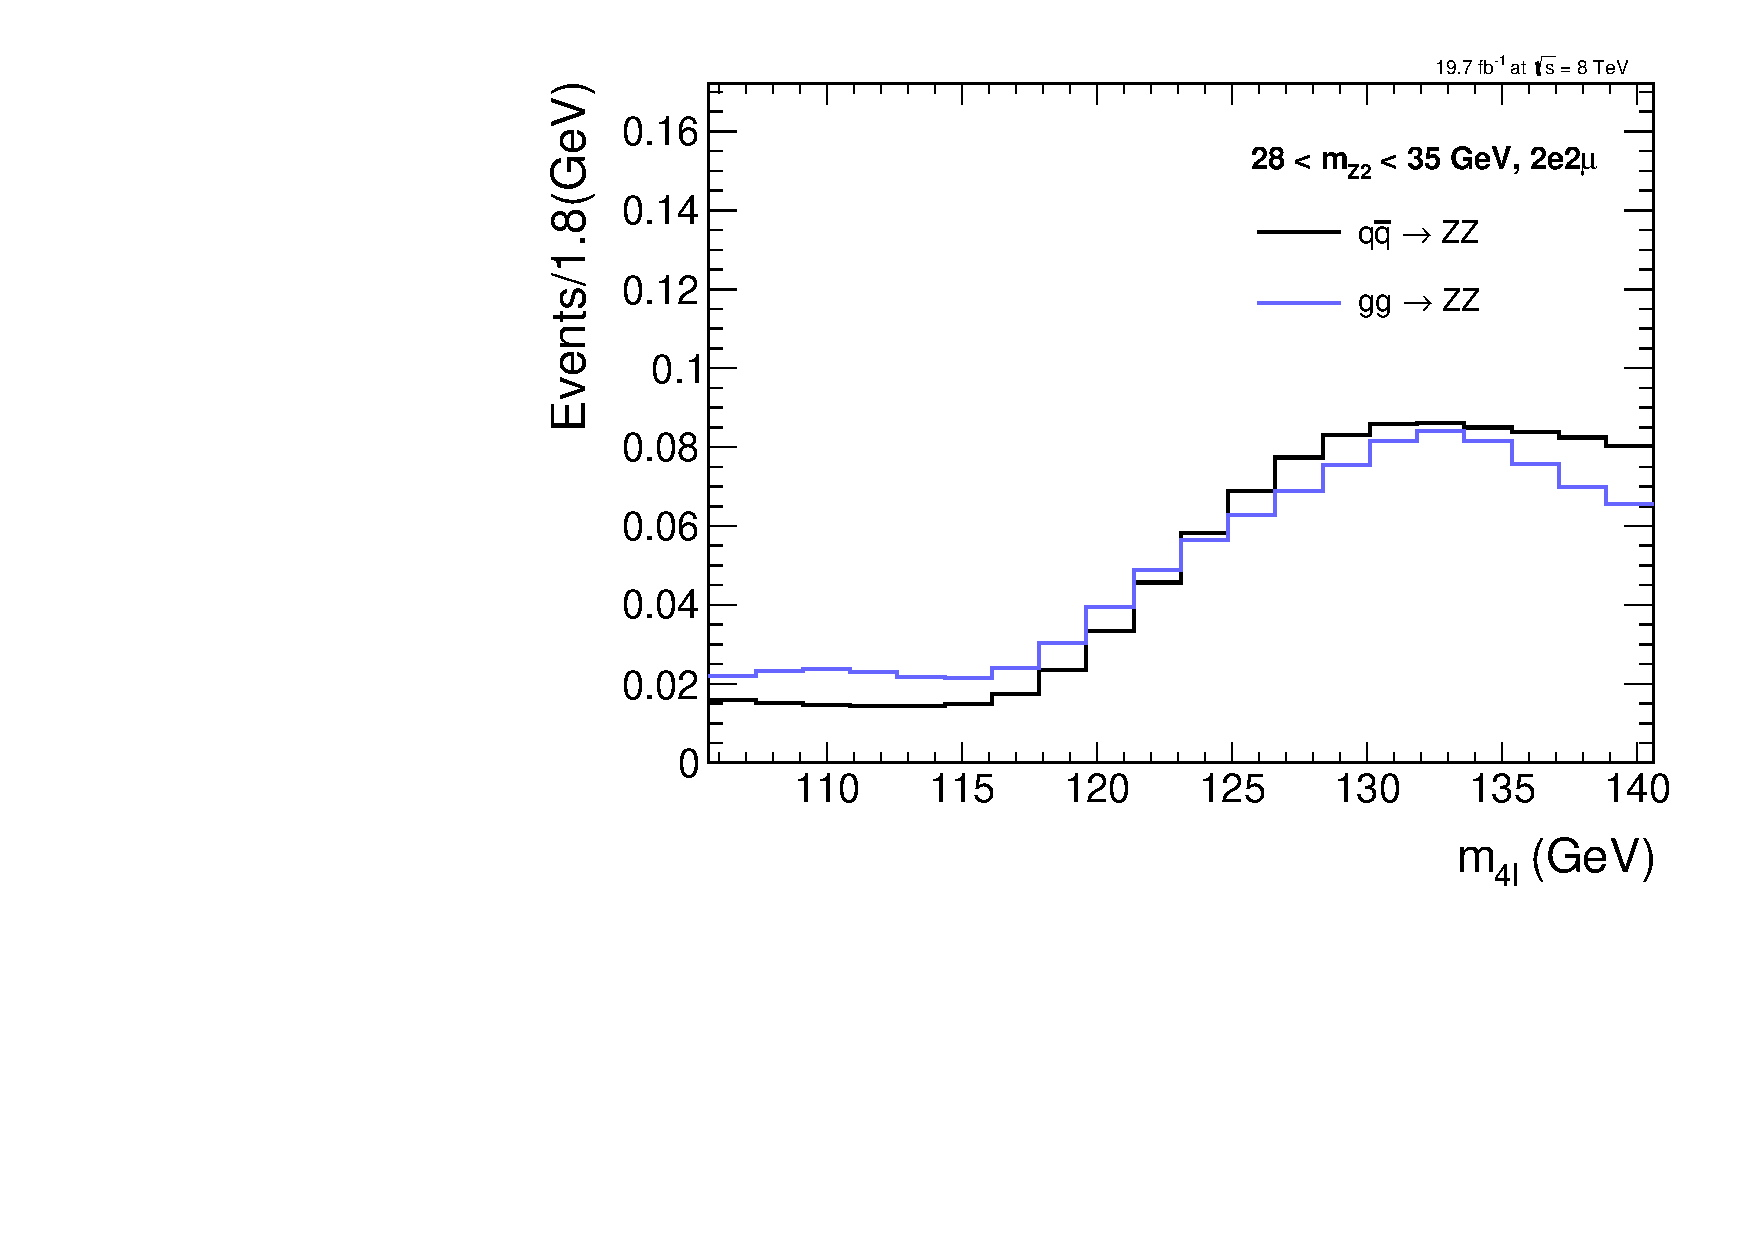
\includegraphics[width=0.30\textwidth,angle=0]{Appendix/figures/XSTemplates_2e2mu_massZ2_28_35_qqZZ_ggZZ.pdf}
      \label{fig:bkg-massZ2-qqZZ-ggZZ-2e2mu:c}
    }
    \subfigure[$28.0 \GeV < \mathrm{m}(\mathrm{Z}_{2}) < 35.0 \GeV$]{
      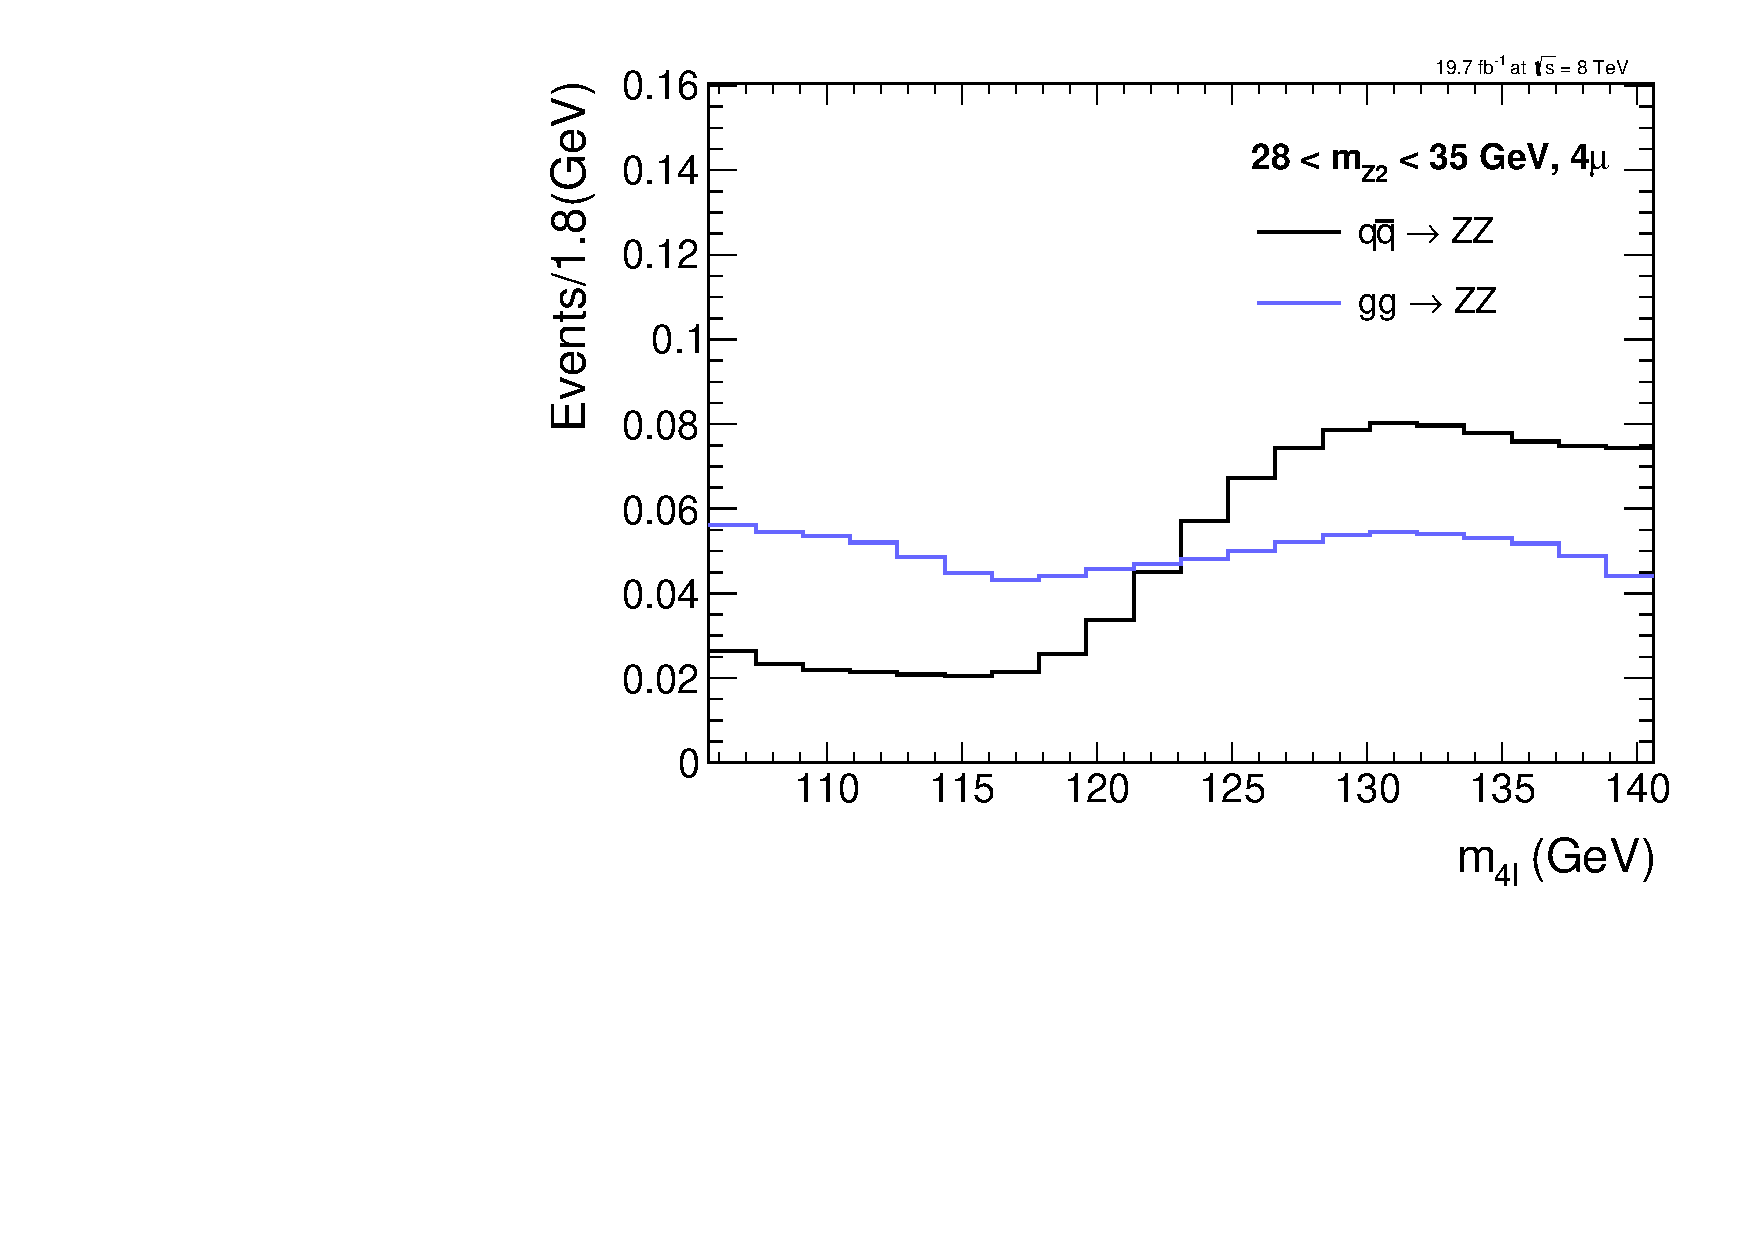
\includegraphics[width=0.30\textwidth,angle=0]{Appendix/figures/XSTemplates_4mu_massZ2_28_35_qqZZ_ggZZ.pdf}
      \label{fig:bkg-massZ2-qqZZ-ggZZ-4mu:c}
    }
    \subfigure[$28.0 \GeV < \mathrm{m}(\mathrm{Z}_{2}) < 35.0 \GeV$]{
      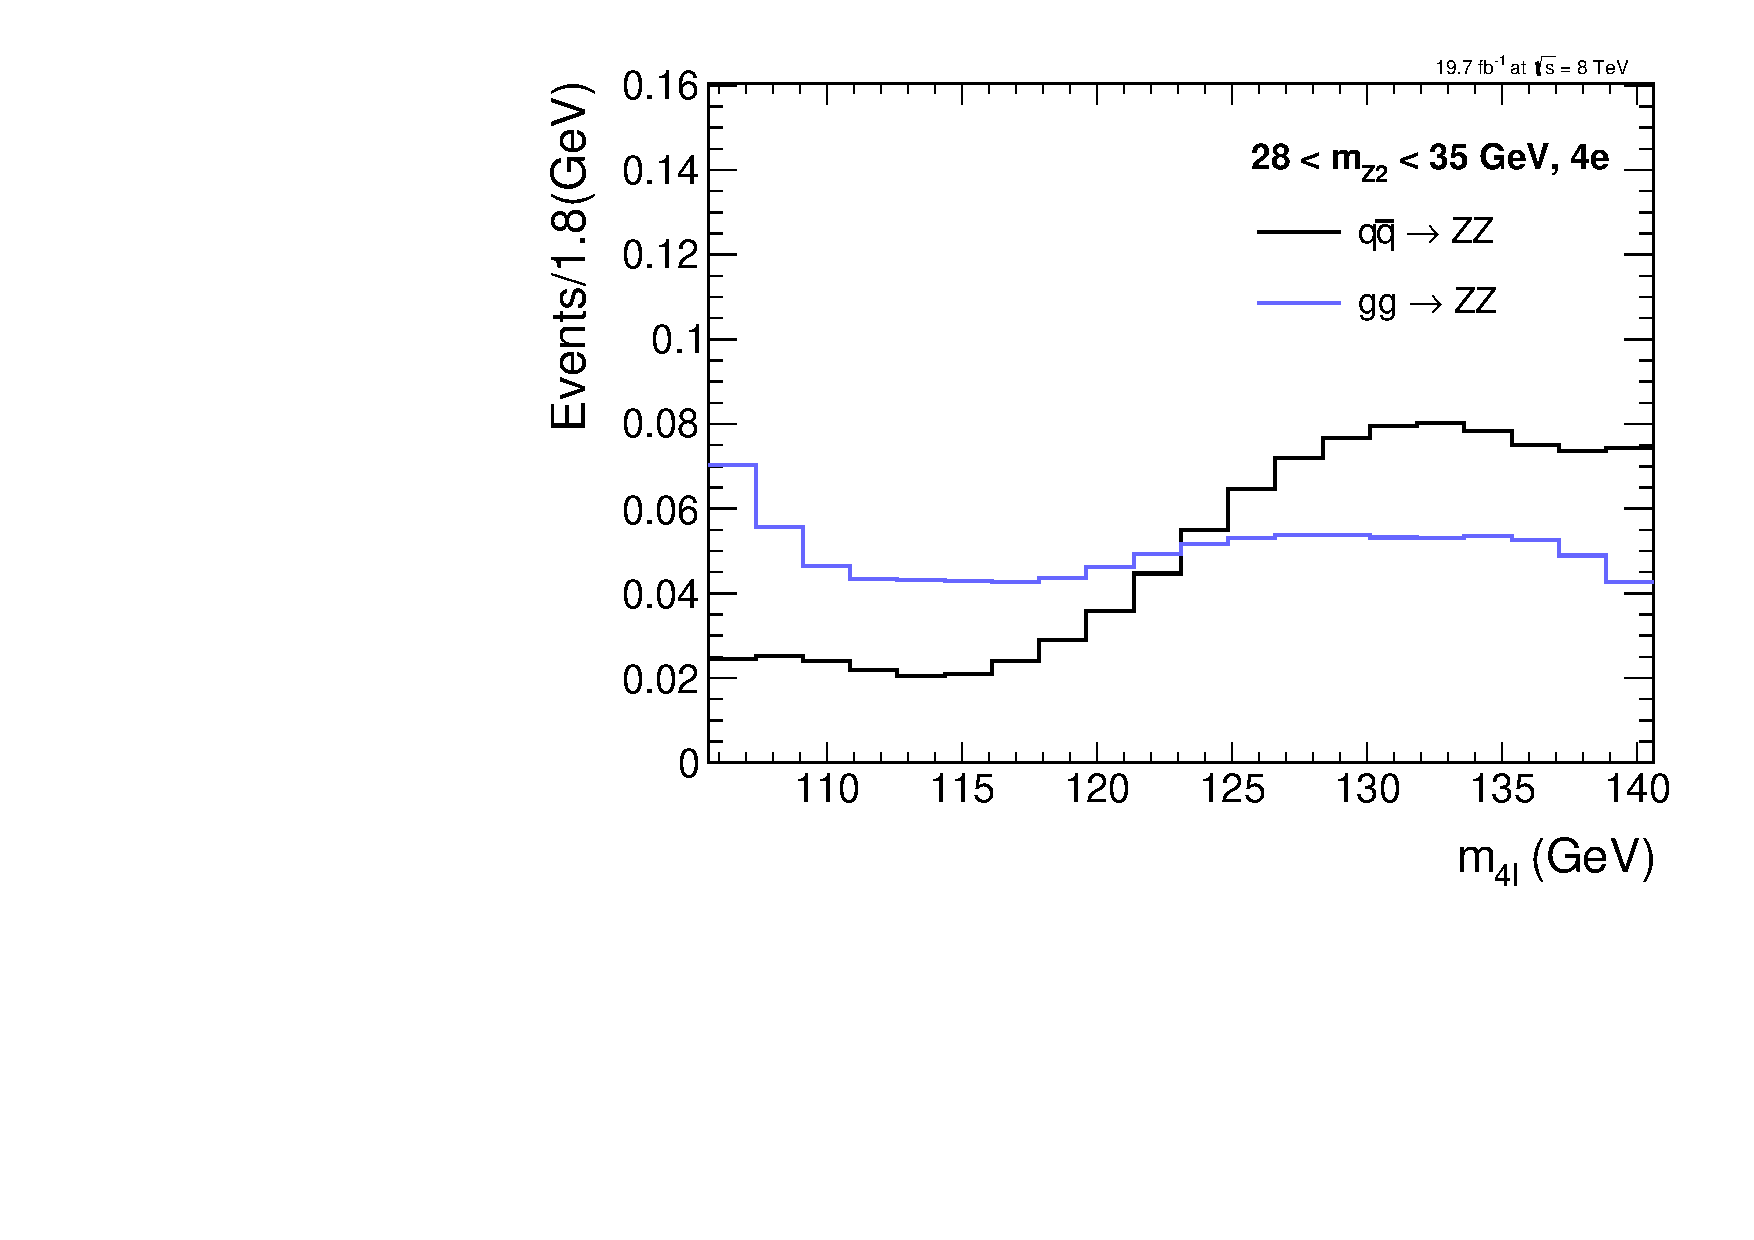
\includegraphics[width=0.30\textwidth,angle=0]{Appendix/figures/XSTemplates_4e_massZ2_28_35_qqZZ_ggZZ.pdf}
      \label{fig:bkg-massZ2-qqZZ-ggZZ-4e:c}
    } \\
    
    \subfigure[$35.0 \GeV < \mathrm{m}(\mathrm{Z}_{2}) < 120.0 \GeV$]{
      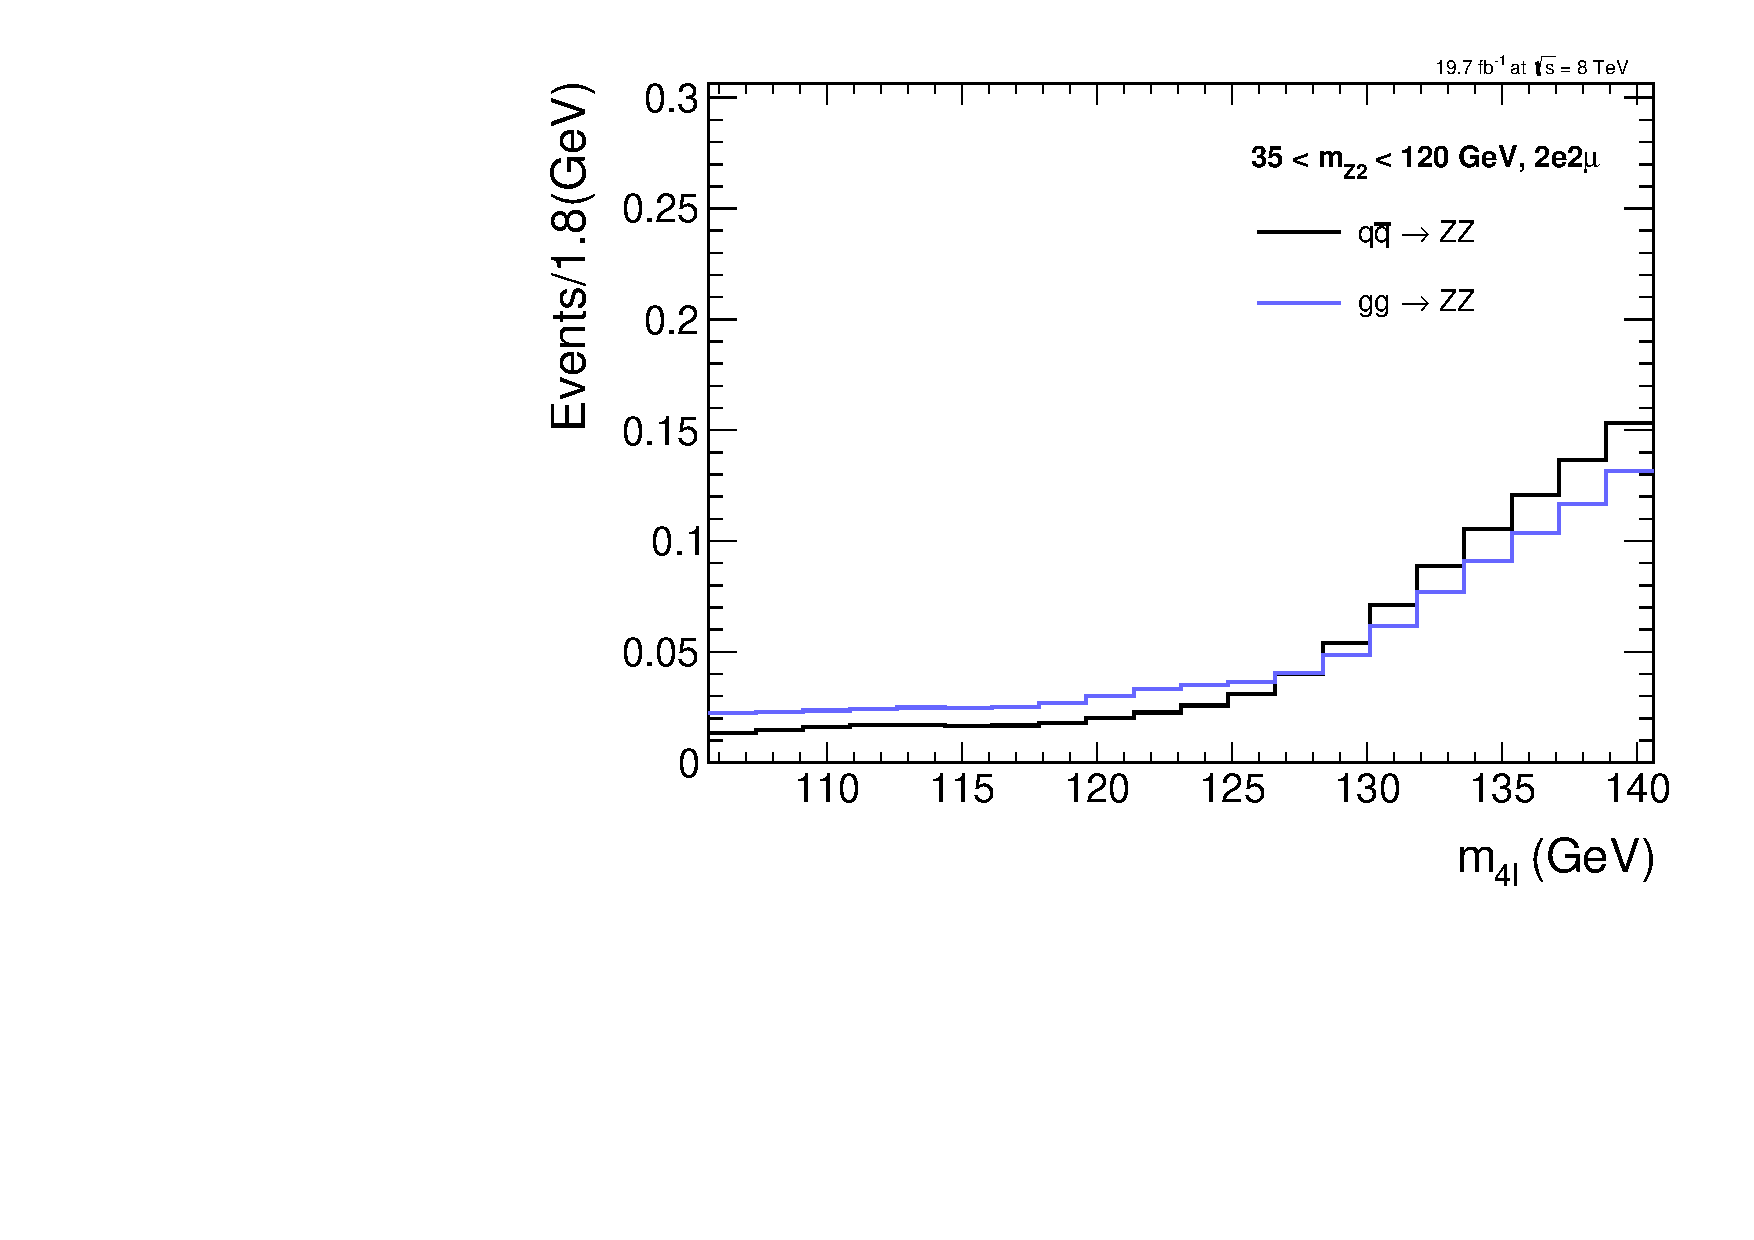
\includegraphics[width=0.30\textwidth,angle=0]{Appendix/figures/XSTemplates_2e2mu_massZ2_35_120_qqZZ_ggZZ.pdf}
      \label{fig:bkg-massZ2-qqZZ-ggZZ-2e2mu:d}
    }
    \subfigure[$35.0 \GeV < \mathrm{m}(\mathrm{Z}_{2}) < 120.0 \GeV$]{
      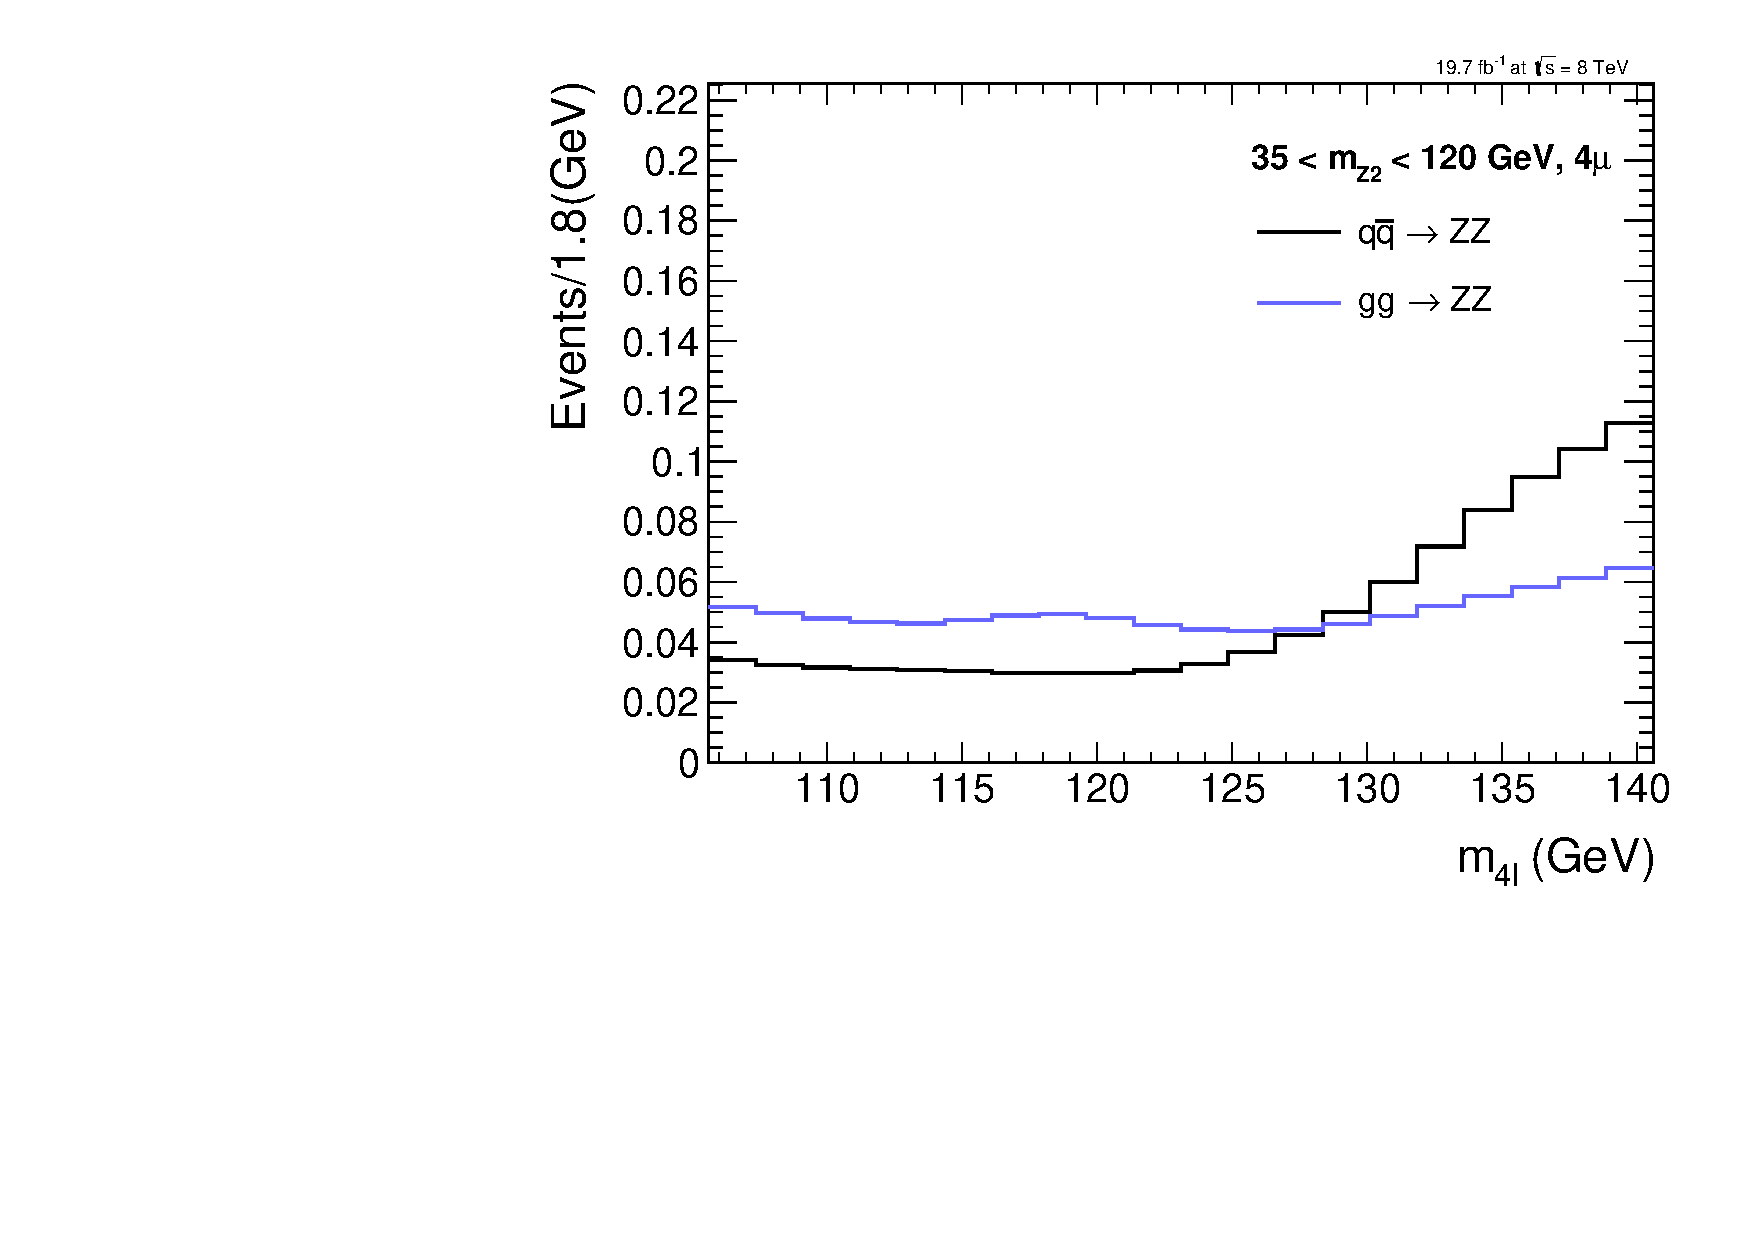
\includegraphics[width=0.30\textwidth,angle=0]{Appendix/figures/XSTemplates_4mu_massZ2_35_120_qqZZ_ggZZ.pdf}
      \label{fig:bkg-massZ2-qqZZ-ggZZ-4mu:d}
    }
    \subfigure[$35.0 \GeV < \mathrm{m}(\mathrm{Z}_{2}) < 120.0 \GeV$]{
      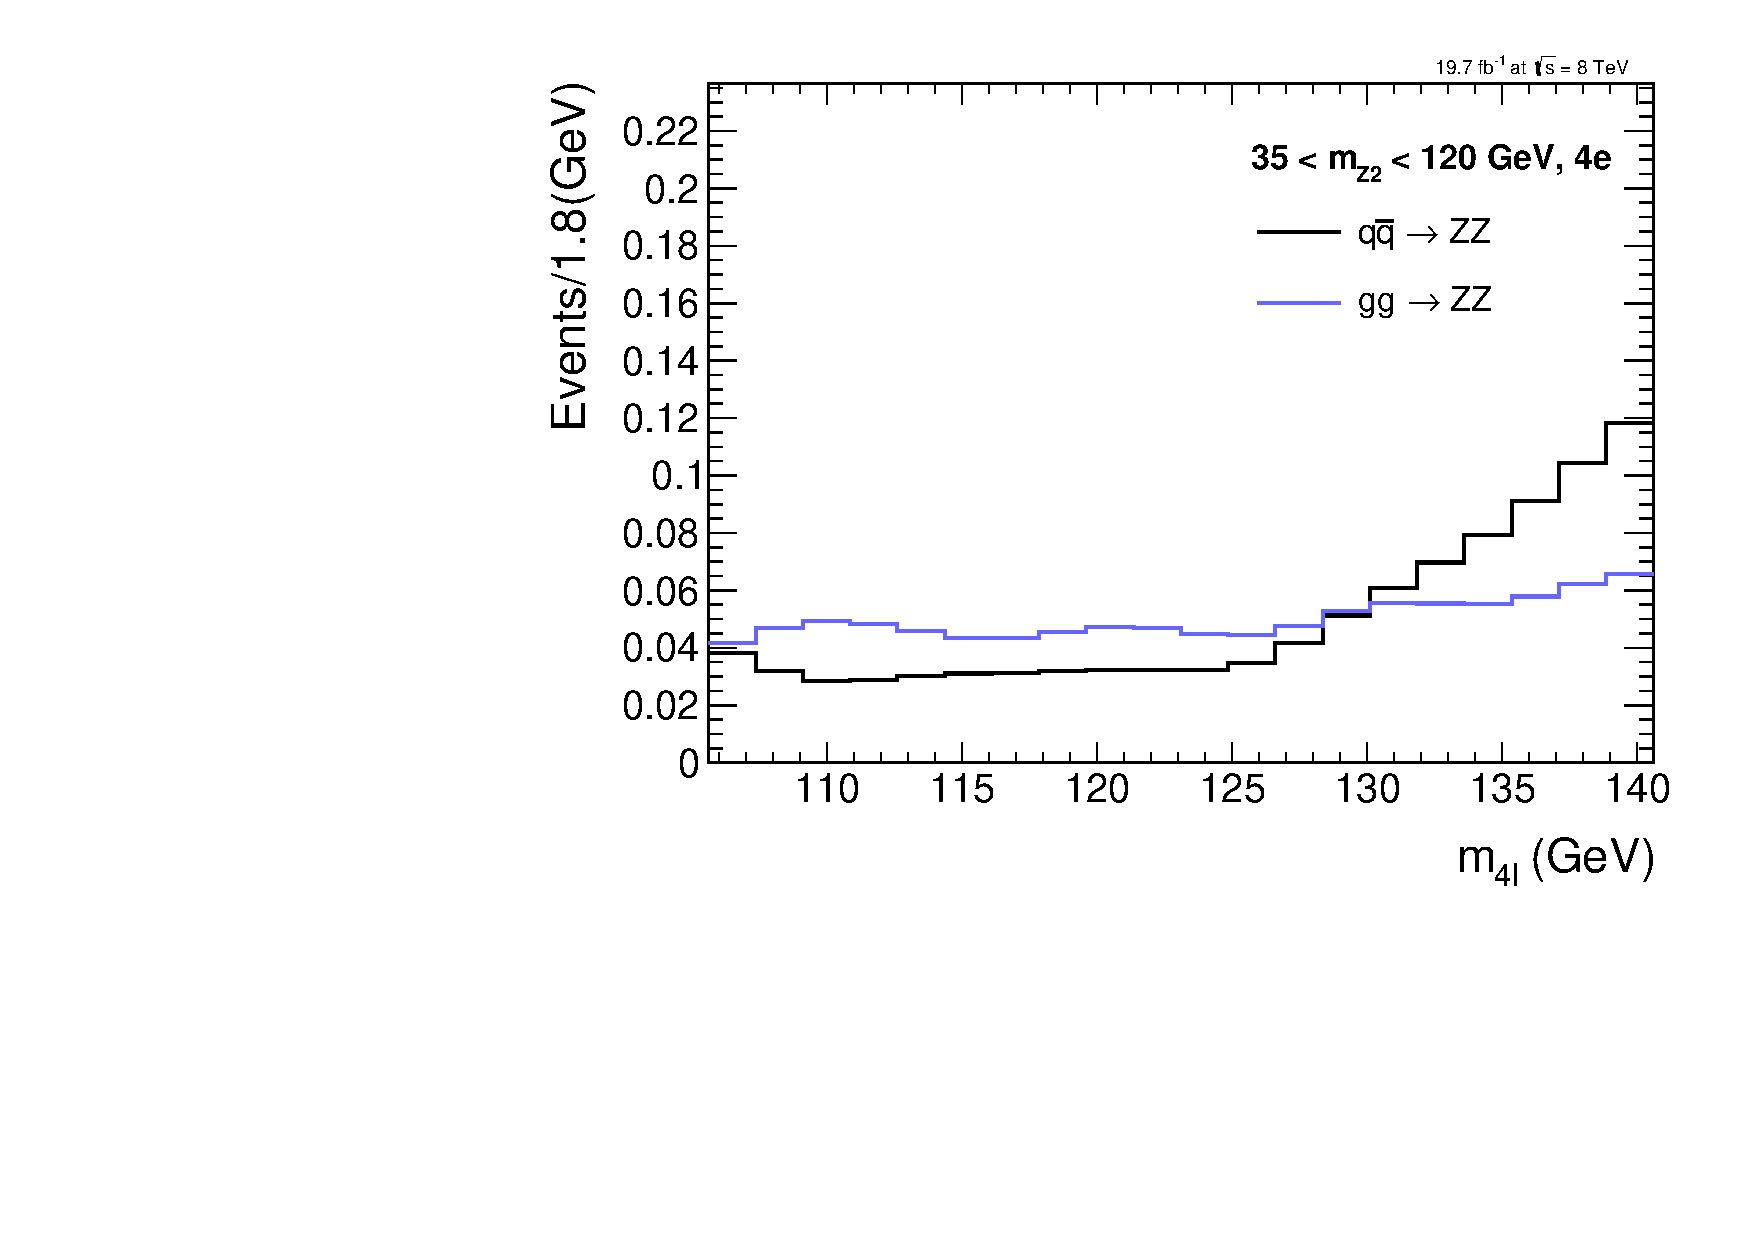
\includegraphics[width=0.30\textwidth,angle=0]{Appendix/figures/XSTemplates_4e_massZ2_35_120_qqZZ_ggZZ.pdf}
      \label{fig:bkg-massZ2-qqZZ-ggZZ-4e:d}
    } \\
    
    \caption{ Distributions of m($4\ell$) for the $qq \rightarrow \mathrm{ZZ}$ and $gg \rightarrow \mathrm{ZZ}$ backgrounds 
    in different bins of $m(\mathrm{Z}_{2})$ for three final states: $2e2\mu$(left), $4\mu$(middle) and $4e$(right).}
  \label{fig:bkg-massZ2-qqZZ-ggZZ}
  
 \end{center}
\end{figure} 

\clearpage

\subsection[Rapidity of the Higgs boson]{Background shapes in bins of $|y(4\ell)|$ }

\begin{figure}[!ht]
  \begin{center}
  
    \subfigure[$0.0 < |y(4\ell)| < 0.4$]{
      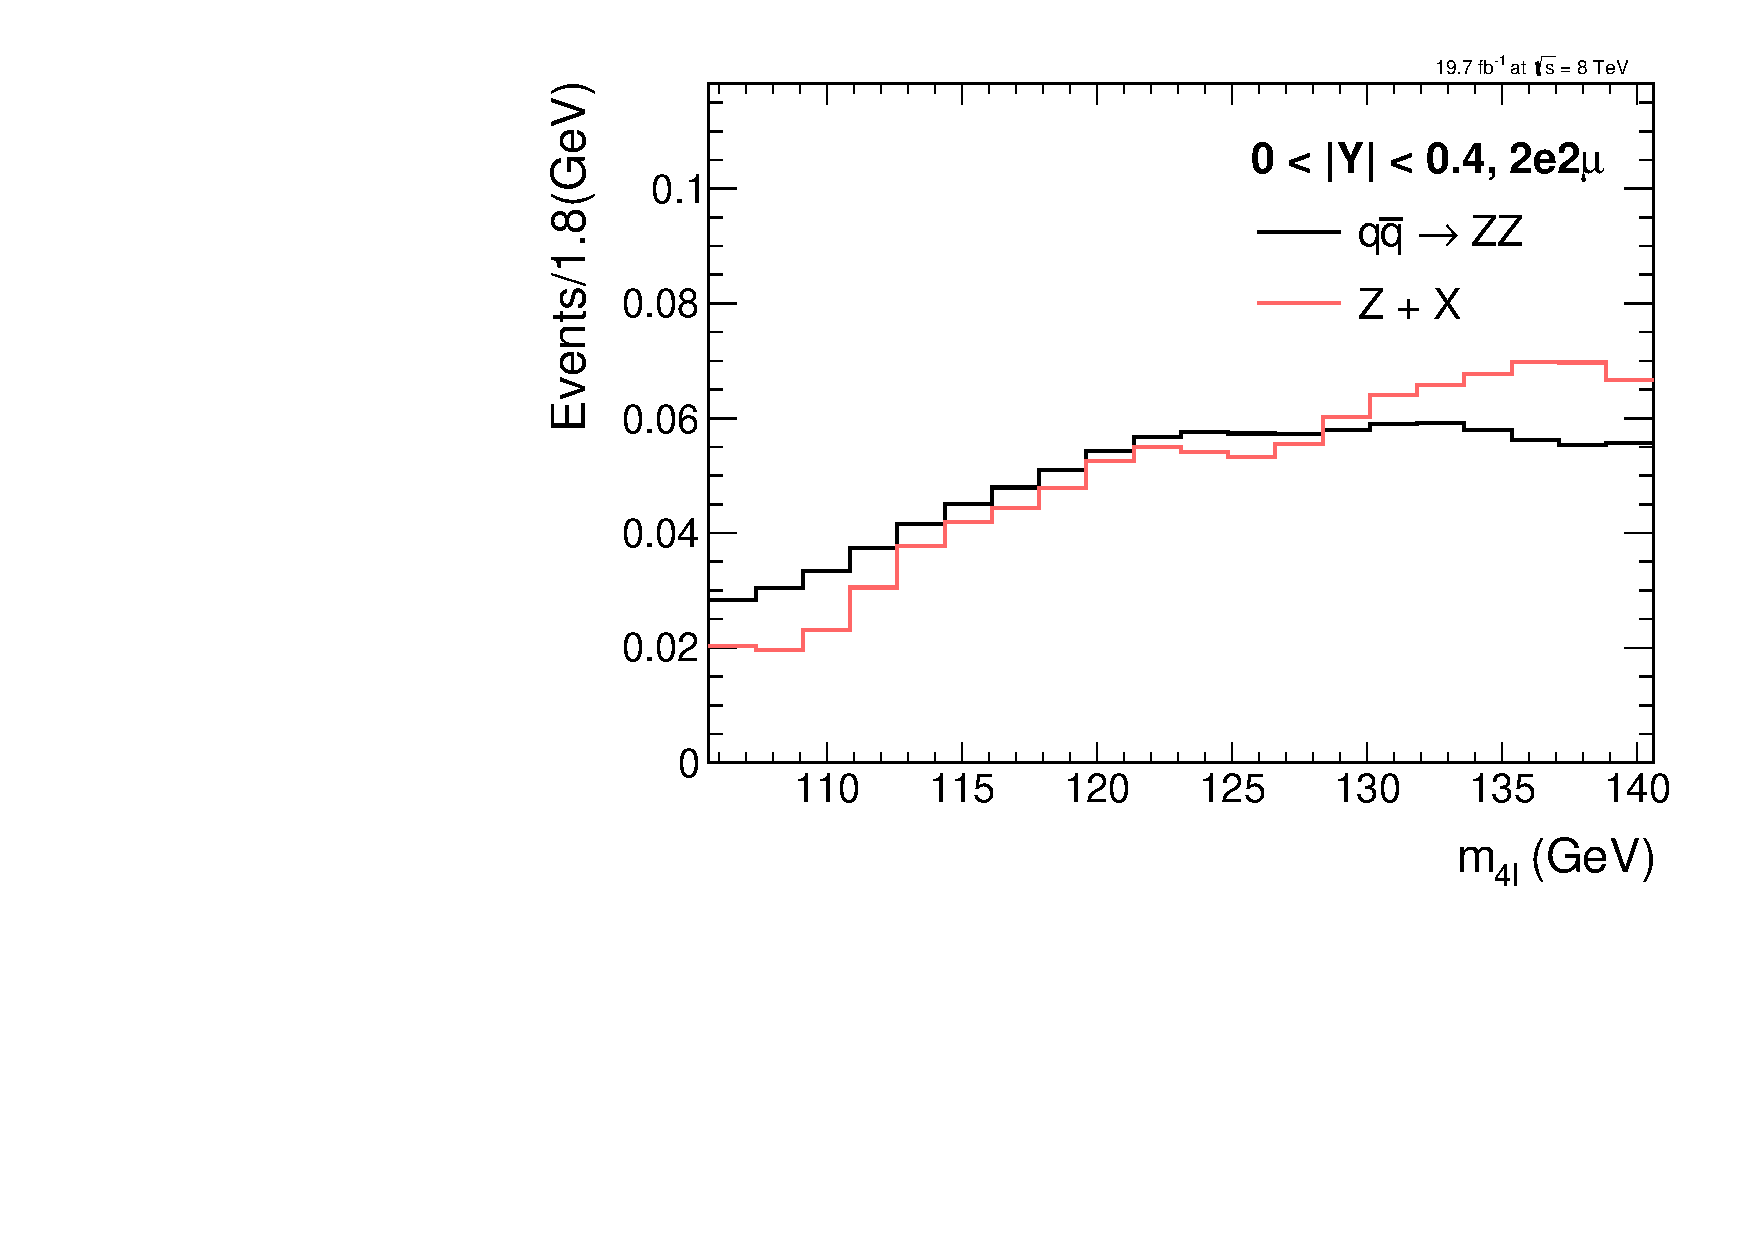
\includegraphics[width=0.30\textwidth,angle=0]{Appendix/figures/XSTemplates_2e2mu_rapidity4l_recobin0_qqZZ_ZJetsCR.pdf}
      \label{fig:bkg-rapidity4l-qqZZ-ZX-2e2mu:a}
    }    
    \subfigure[$0.0 < |y(4\ell)| < 0.4$]{
      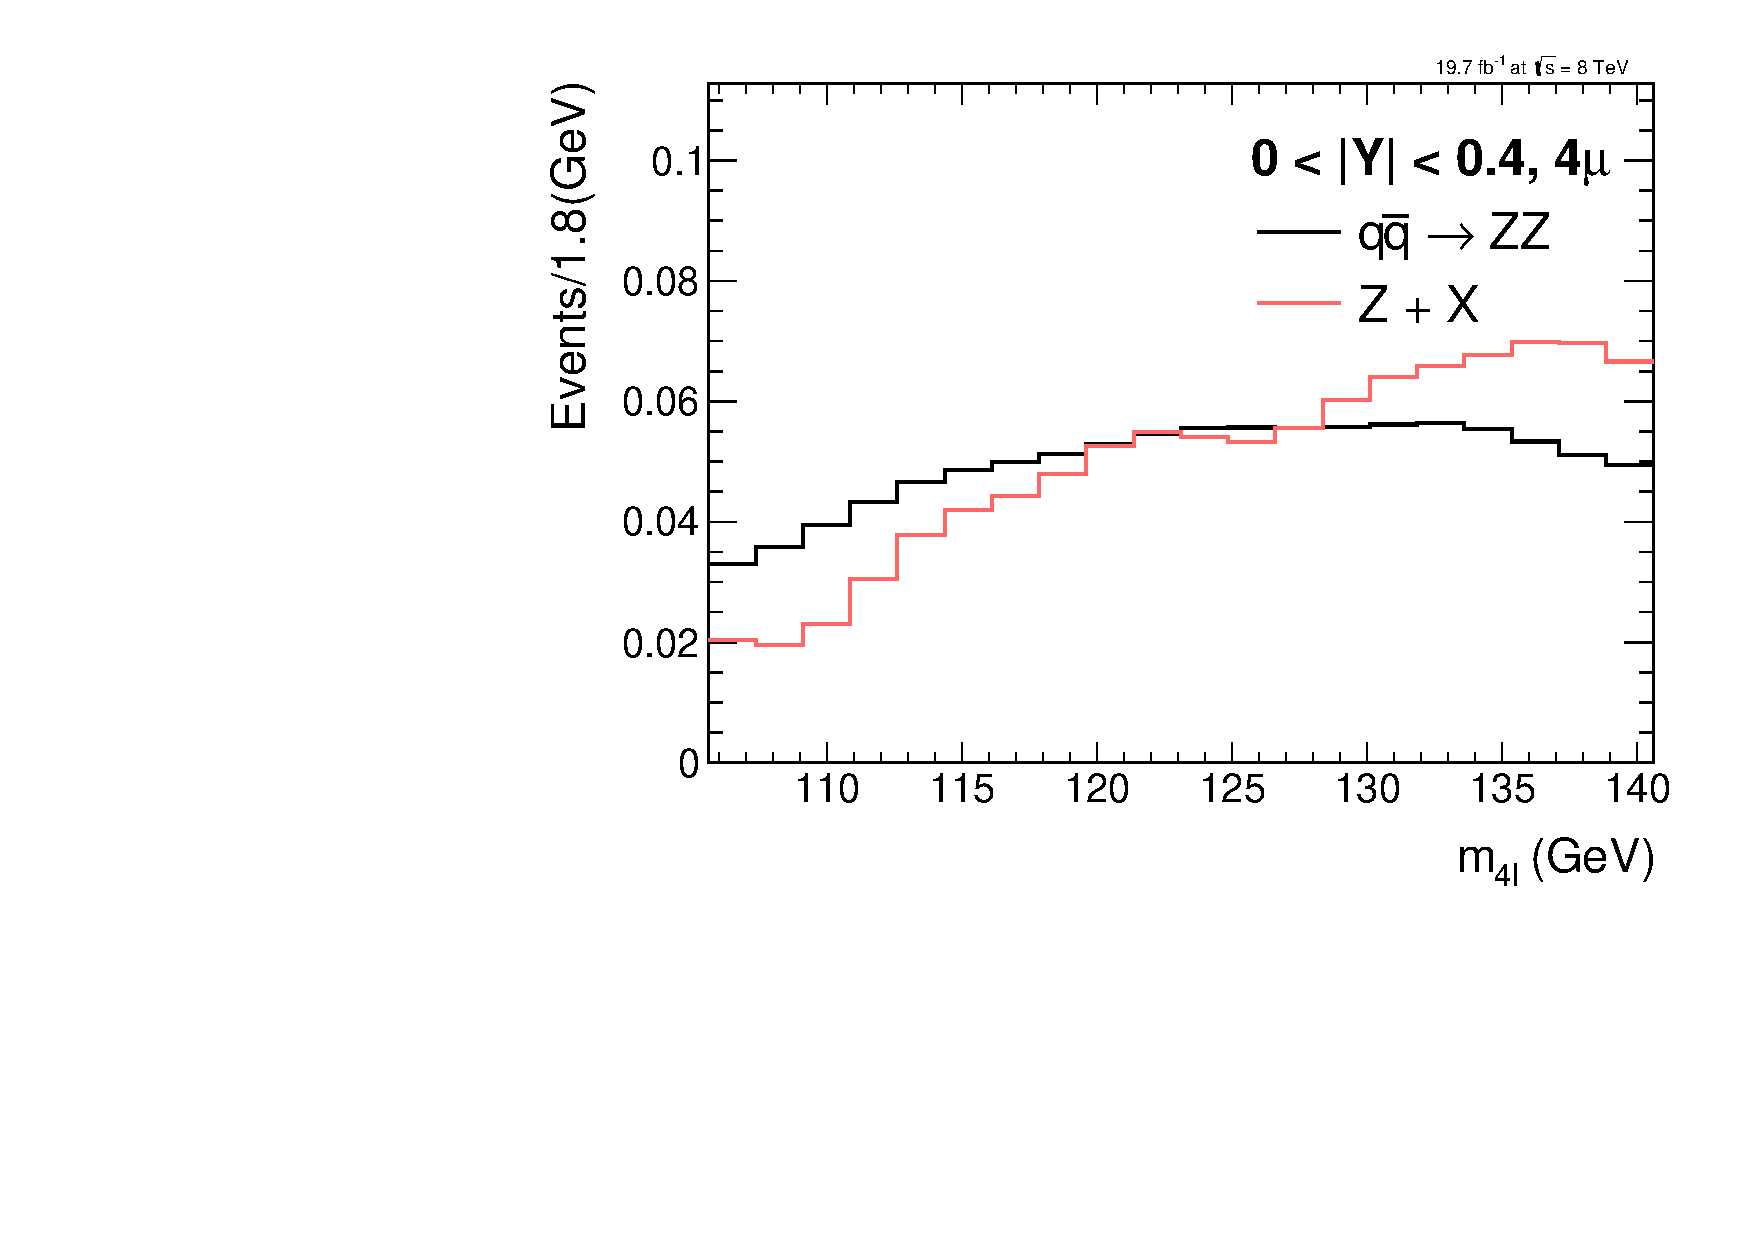
\includegraphics[width=0.30\textwidth,angle=0]{Appendix/figures/XSTemplates_4mu_rapidity4l_recobin0_qqZZ_ZJetsCR.pdf}
      \label{fig:bkg-rapidity4l-qqZZ-ZX-4mu:a}
    }    
    \subfigure[$0.0 < |y(4\ell)| < 0.4$]{
      \includegraphics[width=0.30\textwidth,angle=0]{Appendix/figures/XSTemplates_4e_rapidity4l_recobin0_qqZZ_ZJetsCR.pdf}
      \label{fig:bkg-rapidity4l-qqZZ-ZX-4e:a}
    }    \\

    \subfigure[$0.4 < |y(4\ell)| < 0.8$]{
      \includegraphics[width=0.30\textwidth,angle=0]{Appendix/figures/XSTemplates_2e2mu_rapidity4l_recobin1_qqZZ_ZJetsCR.pdf}
      \label{fig:bkg-rapidity4l-qqZZ-ZX-2e2mu:b}
    }
    \subfigure[$0.4 < |y(4\ell)| < 0.8$]{
      \includegraphics[width=0.30\textwidth,angle=0]{Appendix/figures/XSTemplates_4mu_rapidity4l_recobin1_qqZZ_ZJetsCR.pdf}
      \label{fig:bkg-rapidity4l-qqZZ-ZX-4mu:b}
    } 
    \subfigure[$0.4 < |y(4\ell)| < 0.8$]{
      \includegraphics[width=0.30\textwidth,angle=0]{Appendix/figures/XSTemplates_4e_rapidity4l_recobin1_qqZZ_ZJetsCR.pdf}
      \label{fig:bkg-rapidity4l-qqZZ-ZX-4e:b}
    } \\
    
    \subfigure[$0.8 < |y(4\ell)| < 1.2$]{
      \includegraphics[width=0.30\textwidth,angle=0]{Appendix/figures/XSTemplates_2e2mu_rapidity4l_recobin2_qqZZ_ZJetsCR.pdf}
      \label{fig:bkg-rapidity4l-qqZZ-ZX-2e2mu:c}
    }
    \subfigure[$0.8 < |y(4\ell)| < 1.2$]{
      \includegraphics[width=0.30\textwidth,angle=0]{Appendix/figures/XSTemplates_4mu_rapidity4l_recobin2_qqZZ_ZJetsCR.pdf}
      \label{fig:bkg-rapidity4l-qqZZ-ZX-4mu:c}
    }
    \subfigure[$0.8 < |y(4\ell)| < 1.2$]{
      \includegraphics[width=0.30\textwidth,angle=0]{Appendix/figures/XSTemplates_4e_rapidity4l_recobin2_qqZZ_ZJetsCR.pdf}
      \label{fig:bkg-rapidity4l-qqZZ-ZX-4e:c}
    } \\
    
    \subfigure[$1.2 < |y(4\ell)| < 2.4$]{
      \includegraphics[width=0.30\textwidth,angle=0]{Appendix/figures/XSTemplates_2e2mu_rapidity4l_recobin3_qqZZ_ZJetsCR.pdf}
      \label{fig:bkg-rapidity4l-qqZZ-ZX-2e2mu:d}
    }
    \subfigure[$1.2 < |y(4\ell)| < 2.4$]{
      \includegraphics[width=0.30\textwidth,angle=0]{Appendix/figures/XSTemplates_4mu_rapidity4l_recobin3_qqZZ_ZJetsCR.pdf}
      \label{fig:bkg-rapidity4l-qqZZ-ZX-4mu:d}
    }
    \subfigure[$1.2 < |y(4\ell)| < 2.4$]{
      \includegraphics[width=0.30\textwidth,angle=0]{Appendix/figures/XSTemplates_4e_rapidity4l_recobin3_qqZZ_ZJetsCR.pdf}
      \label{fig:bkg-rapidity4l-qqZZ-ZX-4e:d}
    } \\
    
    \caption{ Distributions of m($4\ell$) for the $qq \rightarrow \mathrm{ZZ}$ and Z+X backgrounds in different bins of $|y(4\ell)|$ 
    for three final states: $2e2\mu$(left), $4\mu$(middle) and $4e$(right).}
  \label{fig:bkg-rapidity4l-qqZZ-ZX}
  
 \end{center}
\end{figure} 

 \clearpage
 
 \begin{figure}[!ht]
  \begin{center}
  
    \subfigure[$0.0 < |y(4\ell)| < 0.4$]{
      \includegraphics[width=0.30\textwidth,angle=0]{Appendix/figures/XSTemplates_2e2mu_rapidity4l_recobin0_qqZZ_ggZZ.pdf}
      \label{fig:bkg-rapidity4l-qqZZ-ggZZ-2e2mu:a}
    }    
    \subfigure[$0.0 < |y(4\ell)| < 0.4$]{
      \includegraphics[width=0.30\textwidth,angle=0]{Appendix/figures/XSTemplates_4mu_rapidity4l_recobin0_qqZZ_ggZZ.pdf}
      \label{fig:bkg-rapidity4l-qqZZ-ggZZ-4mu:a}
    }    
    \subfigure[$0.0 < |y(4\ell)| < 0.4$]{
      \includegraphics[width=0.30\textwidth,angle=0]{Appendix/figures/XSTemplates_4e_rapidity4l_recobin0_qqZZ_ggZZ.pdf}
      \label{fig:bkg-rapidity4l-qqZZ-ggZZ-4e:a}
    }    \\

    \subfigure[$0.4 < |y(4\ell)| < 0.8$]{
      \includegraphics[width=0.30\textwidth,angle=0]{Appendix/figures/XSTemplates_2e2mu_rapidity4l_recobin1_qqZZ_ggZZ.pdf}
      \label{fig:bkg-rapidity4l-qqZZ-ggZZ-2e2mu:b}
    }
    \subfigure[$0.4 < |y(4\ell)| < 0.8$]{
      \includegraphics[width=0.30\textwidth,angle=0]{Appendix/figures/XSTemplates_4mu_rapidity4l_recobin1_qqZZ_ggZZ.pdf}
      \label{fig:bkg-rapidity4l-qqZZ-ggZZ-4mu:b}
    } 
    \subfigure[$0.4 < |y(4\ell)| < 0.8$]{
      \includegraphics[width=0.30\textwidth,angle=0]{Appendix/figures/XSTemplates_4e_rapidity4l_recobin1_qqZZ_ggZZ.pdf}
      \label{fig:bkg-rapidity4l-qqZZ-ggZZ-4e:b}
    } \\
    
    \subfigure[$0.8 < |y(4\ell)| < 1.2$]{
      \includegraphics[width=0.30\textwidth,angle=0]{Appendix/figures/XSTemplates_2e2mu_rapidity4l_recobin2_qqZZ_ggZZ.pdf}
      \label{fig:bkg-rapidity4l-qqZZ-ggZZ-2e2mu:c}
    }
    \subfigure[$0.8 < |y(4\ell)| < 1.2$]{
      \includegraphics[width=0.30\textwidth,angle=0]{Appendix/figures/XSTemplates_4mu_rapidity4l_recobin2_qqZZ_ggZZ.pdf}
      \label{fig:bkg-rapidity4l-qqZZ-ggZZ-4mu:c}
    }
    \subfigure[$0.8 < |y(4\ell)| < 1.2$]{
      \includegraphics[width=0.30\textwidth,angle=0]{Appendix/figures/XSTemplates_4e_rapidity4l_recobin2_qqZZ_ggZZ.pdf}
      \label{fig:bkg-rapidity4l-qqZZ-ggZZ-4e:c}
    } \\
    
    \subfigure[$1.2 < |y(4\ell)| < 2.4$]{
      \includegraphics[width=0.30\textwidth,angle=0]{Appendix/figures/XSTemplates_2e2mu_rapidity4l_recobin3_qqZZ_ggZZ.pdf}
      \label{fig:bkg-rapidity4l-qqZZ-ggZZ-2e2mu:d}
    }
    \subfigure[$1.2 < |y(4\ell)| < 2.4$]{
      \includegraphics[width=0.30\textwidth,angle=0]{Appendix/figures/XSTemplates_4mu_rapidity4l_recobin3_qqZZ_ggZZ.pdf}
      \label{fig:bkg-rapidity4l-qqZZ-ggZZ-4mu:d}
    }
    \subfigure[$1.2 < |y(4\ell)| < 2.4$]{
      \includegraphics[width=0.30\textwidth,angle=0]{Appendix/figures/XSTemplates_4e_rapidity4l_recobin3_qqZZ_ggZZ.pdf}
      \label{fig:bkg-rapidity4l-qqZZ-ggZZ-4e:d}
    } \\
    
    \caption{ Distributions of m($4\ell$) for the $qq \rightarrow \mathrm{ZZ}$ and $gg \rightarrow \mathrm{ZZ}$ backgrounds 
    in different bins of $|y(4\ell)|$ for three final states: $2e2\mu$(left), $4\mu$(middle) and $4e$(right).}
  \label{fig:bkg-rapidity4l-qqZZ-ggZZ}
  
 \end{center}
\end{figure} 

\clearpage


\subsection[Helicity angle theta*]{Background shapes in bins of $|\cos \theta^{*}|$ }

\begin{figure}[!ht]
  \begin{center}
  
    \subfigure[$0.0 < |\cos \theta^{*}| < 0.25$]{
      \includegraphics[width=0.30\textwidth,angle=0]{Appendix/figures/XSTemplates_2e2mu_cosThetaStar_recobin0_qqZZ_ZJetsCR.pdf}
      \label{fig:bkg-cosThetaStar-qqZZ-ZX-2e2mu:a}
    }    
    \subfigure[$0.0 < |\cos \theta^{*}| < 0.25$]{
      \includegraphics[width=0.30\textwidth,angle=0]{Appendix/figures/XSTemplates_4mu_cosThetaStar_recobin0_qqZZ_ZJetsCR.pdf}
      \label{fig:bkg-cosThetaStar-qqZZ-ZX-4mu:a}
    }    
    \subfigure[$0.0 < |\cos \theta^{*}| < 0.25$]{
      \includegraphics[width=0.30\textwidth,angle=0]{Appendix/figures/XSTemplates_4e_cosThetaStar_recobin0_qqZZ_ZJetsCR.pdf}
      \label{fig:bkg-cosThetaStar-qqZZ-ZX-4e:a}
    }    \\

    \subfigure[$0.25 < |\cos \theta^{*}| < 0.50$]{
      \includegraphics[width=0.30\textwidth,angle=0]{Appendix/figures/XSTemplates_2e2mu_cosThetaStar_recobin1_qqZZ_ZJetsCR.pdf}
      \label{fig:bkg-cosThetaStar-qqZZ-ZX-2e2mu:b}
    }
    \subfigure[$0.25 < |\cos \theta^{*}| < 0.50$]{
      \includegraphics[width=0.30\textwidth,angle=0]{Appendix/figures/XSTemplates_4mu_cosThetaStar_recobin1_qqZZ_ZJetsCR.pdf}
      \label{fig:bkg-cosThetaStar-qqZZ-ZX-4mu:b}
    } 
    \subfigure[$0.25 < |\cos \theta^{*}| < 0.50$]{
      \includegraphics[width=0.30\textwidth,angle=0]{Appendix/figures/XSTemplates_4e_cosThetaStar_recobin1_qqZZ_ZJetsCR.pdf}
      \label{fig:bkg-cosThetaStar-qqZZ-ZX-4e:b}
    } \\
    
    \subfigure[$0.50 < |\cos \theta^{*}| < 0.75$]{
      \includegraphics[width=0.30\textwidth,angle=0]{Appendix/figures/XSTemplates_2e2mu_cosThetaStar_recobin2_qqZZ_ZJetsCR.pdf}
      \label{fig:bkg-cosThetaStar-qqZZ-ZX-2e2mu:c}
    }
    \subfigure[$0.50 < |\cos \theta^{*}| < 0.75$]{
      \includegraphics[width=0.30\textwidth,angle=0]{Appendix/figures/XSTemplates_4mu_cosThetaStar_recobin2_qqZZ_ZJetsCR.pdf}
      \label{fig:bkg-cosThetaStar-qqZZ-ZX-4mu:c}
    }
    \subfigure[$0.50 < |\cos \theta^{*}| < 0.75$]{
      \includegraphics[width=0.30\textwidth,angle=0]{Appendix/figures/XSTemplates_4e_cosThetaStar_recobin2_qqZZ_ZJetsCR.pdf}
      \label{fig:bkg-cosThetaStar-qqZZ-ZX-4e:c}
    } \\
    
    \subfigure[$0.75 < |\cos \theta^{*}| < 1.0$]{
      \includegraphics[width=0.30\textwidth,angle=0]{Appendix/figures/XSTemplates_2e2mu_cosThetaStar_recobin3_qqZZ_ZJetsCR.pdf}
      \label{fig:bkg-cosThetaStar-qqZZ-ZX-2e2mu:d}
    }
    \subfigure[$0.75 < |\cos \theta^{*}| < 1.0$]{
      \includegraphics[width=0.30\textwidth,angle=0]{Appendix/figures/XSTemplates_4mu_cosThetaStar_recobin3_qqZZ_ZJetsCR.pdf}
      \label{fig:bkg-cosThetaStar-qqZZ-ZX-4mu:d}
    }
    \subfigure[$0.75 < |\cos \theta^{*}| < 1.0$]{
      \includegraphics[width=0.30\textwidth,angle=0]{Appendix/figures/XSTemplates_4e_cosThetaStar_recobin3_qqZZ_ZJetsCR.pdf}
      \label{fig:bkg-cosThetaStar-qqZZ-ZX-4e:d}
    } \\
    
    \caption{ Distributions of m($4\ell$) for the $qq \rightarrow \mathrm{ZZ}$ and Z+X backgrounds in different bins of  $|\cos \theta^{*}|$
    for three final states: $2e2\mu$(left), $4\mu$(middle) and $4e$(right).}
  \label{fig:bkg-cosThetaStar-qqZZ-ZX}
  
 \end{center}
\end{figure} 

 \clearpage
 
 \begin{figure}[!ht]
  \begin{center}
  
    \subfigure[$0.0 < |\cos \theta^{*}| < 0.25$]{
      \includegraphics[width=0.30\textwidth,angle=0]{Appendix/figures/XSTemplates_2e2mu_cosThetaStar_recobin0_qqZZ_ggZZ.pdf}
      \label{fig:bkg-cosThetaStar-qqZZ-ggZZ-2e2mu:a}
    }    
    \subfigure[$0.0 < |\cos \theta^{*}| < 0.25$]{
      \includegraphics[width=0.30\textwidth,angle=0]{Appendix/figures/XSTemplates_4mu_cosThetaStar_recobin0_qqZZ_ggZZ.pdf}
      \label{fig:bkg-cosThetaStar-qqZZ-ggZZ-4mu:a}
    }    
    \subfigure[$0.0 < |\cos \theta^{*}| < 0.25$]{
      \includegraphics[width=0.30\textwidth,angle=0]{Appendix/figures/XSTemplates_4e_cosThetaStar_recobin0_qqZZ_ggZZ.pdf}
      \label{fig:bkg-cosThetaStar-qqZZ-ggZZ-4e:a}
    }    \\

    \subfigure[$0.25 < |\cos \theta^{*}| < 0.50$]{
      \includegraphics[width=0.30\textwidth,angle=0]{Appendix/figures/XSTemplates_2e2mu_cosThetaStar_recobin1_qqZZ_ggZZ.pdf}
      \label{fig:bkg-cosThetaStar-qqZZ-ggZZ-2e2mu:b}
    }
    \subfigure[$0.25 < |\cos \theta^{*}| < 0.50$]{
      \includegraphics[width=0.30\textwidth,angle=0]{Appendix/figures/XSTemplates_4mu_cosThetaStar_recobin1_qqZZ_ggZZ.pdf}
      \label{fig:bkg-cosThetaStar-qqZZ-ggZZ-4mu:b}
    } 
    \subfigure[$0.25 < |\cos \theta^{*}| < 0.50$]{
      \includegraphics[width=0.30\textwidth,angle=0]{Appendix/figures/XSTemplates_4e_cosThetaStar_recobin1_qqZZ_ggZZ.pdf}
      \label{fig:bkg-cosThetaStar-qqZZ-ggZZ-4e:b}
    } \\
    
    \subfigure[$0.50 < |\cos \theta^{*}| < 0.75$]{
      \includegraphics[width=0.30\textwidth,angle=0]{Appendix/figures/XSTemplates_2e2mu_cosThetaStar_recobin2_qqZZ_ggZZ.pdf}
      \label{fig:bkg-cosThetaStar-qqZZ-ggZZ-2e2mu:c}
    }
    \subfigure[$0.50 < |\cos \theta^{*}| < 0.75$]{
      \includegraphics[width=0.30\textwidth,angle=0]{Appendix/figures/XSTemplates_4mu_cosThetaStar_recobin2_qqZZ_ggZZ.pdf}
      \label{fig:bkg-cosThetaStar-qqZZ-ggZZ-4mu:c}
    }
    \subfigure[$0.50 < |\cos \theta^{*}| < 0.75$]{
      \includegraphics[width=0.30\textwidth,angle=0]{Appendix/figures/XSTemplates_4e_cosThetaStar_recobin2_qqZZ_ggZZ.pdf}
      \label{fig:bkg-cosThetaStar-qqZZ-ggZZ-4e:c}
    } \\
    
    \subfigure[$0.75 < |\cos \theta^{*}| < 1.0$]{
      \includegraphics[width=0.30\textwidth,angle=0]{Appendix/figures/XSTemplates_2e2mu_cosThetaStar_recobin3_qqZZ_ggZZ.pdf}
      \label{fig:bkg-cosThetaStar-qqZZ-ggZZ-2e2mu:d}
    }
    \subfigure[$0.75 < |\cos \theta^{*}| < 1.0$]{
      \includegraphics[width=0.30\textwidth,angle=0]{Appendix/figures/XSTemplates_4mu_cosThetaStar_recobin3_qqZZ_ggZZ.pdf}
      \label{fig:bkg-cosThetaStar-qqZZ-ggZZ-4mu:d}
    }
    \subfigure[$0.75 < |\cos \theta^{*}| < 1.0$]{
      \includegraphics[width=0.30\textwidth,angle=0]{Appendix/figures/XSTemplates_4e_cosThetaStar_recobin3_qqZZ_ggZZ.pdf}
      \label{fig:bkg-cosThetaStar-qqZZ-ggZZ-4e:d}
    } \\
    
    \caption{ Distributions of m($4\ell$) for the $qq \rightarrow \mathrm{ZZ}$ and $gg \rightarrow \mathrm{ZZ}$ backgrounds 
    in different bins of  $|\cos \theta^{*}|$ for three final states: $2e2\mu$(left), $4\mu$(middle) and $4e$(right).}
  \label{fig:bkg-cosThetaStar-qqZZ-ggZZ}
  
 \end{center}
\end{figure} 

\clearpage


\subsection[Number of jets]{Background shapes in bins of $N_{\rm jets}$ }

\begin{figure}[!ht]
  \begin{center}
  
    \subfigure[$\mathrm{N(jets)}=0$]{
      \includegraphics[width=0.30\textwidth,angle=0]{Appendix/figures/XSTemplates_2e2mu_njets_reco_pt30_eta4p7_0_1_qqZZ_ZJetsCR.pdf}
      \label{fig:bkg-njets_reco_pt30_eta4p7-qqZZ-ZX-2e2mu:a}
    }    
    \subfigure[$\mathrm{N(jets)}=0$]{
      \includegraphics[width=0.30\textwidth,angle=0]{Appendix/figures/XSTemplates_4mu_njets_reco_pt30_eta4p7_0_1_qqZZ_ZJetsCR.pdf}
      \label{fig:bkg-njets_reco_pt30_eta4p7-qqZZ-ZX-4mu:a}
    }    
    \subfigure[$\mathrm{N(jets)}=0$]{
      \includegraphics[width=0.30\textwidth,angle=0]{Appendix/figures/XSTemplates_4e_njets_reco_pt30_eta4p7_0_1_qqZZ_ZJetsCR.pdf}
      \label{fig:bkg-njets_reco_pt30_eta4p7-qqZZ-ZX-4e:a}
    }    \\

    \subfigure[$\mathrm{N(jets)}=1$]{
      \includegraphics[width=0.30\textwidth,angle=0]{Appendix/figures/XSTemplates_2e2mu_njets_reco_pt30_eta4p7_1_2_qqZZ_ZJetsCR.pdf}
      \label{fig:bkg-njets_reco_pt30_eta4p7-qqZZ-ZX-2e2mu:b}
    }
    \subfigure[$\mathrm{N(jets)}=1$]{
      \includegraphics[width=0.30\textwidth,angle=0]{Appendix/figures/XSTemplates_4mu_njets_reco_pt30_eta4p7_1_2_qqZZ_ZJetsCR.pdf}
      \label{fig:bkg-njets_reco_pt30_eta4p7-qqZZ-ZX-4mu:b}
    } 
    \subfigure[$\mathrm{N(jets)}=1$]{
      \includegraphics[width=0.30\textwidth,angle=0]{Appendix/figures/XSTemplates_4e_njets_reco_pt30_eta4p7_1_2_qqZZ_ZJetsCR.pdf}
      \label{fig:bkg-njets_reco_pt30_eta4p7-qqZZ-ZX-4e:b}
    } \\
    
    \subfigure[$\mathrm{N(jets)}=2$]{
      \includegraphics[width=0.30\textwidth,angle=0]{Appendix/figures/XSTemplates_2e2mu_njets_reco_pt30_eta4p7_2_3_qqZZ_ZJetsCR.pdf}
      \label{fig:bkg-njets_reco_pt30_eta4p7-qqZZ-ZX-2e2mu:c}
    }
    \subfigure[$\mathrm{N(jets)}=2$]{
      \includegraphics[width=0.30\textwidth,angle=0]{Appendix/figures/XSTemplates_4mu_njets_reco_pt30_eta4p7_2_3_qqZZ_ZJetsCR.pdf}
      \label{fig:bkg-njets_reco_pt30_eta4p7-qqZZ-ZX-4mu:c}
    }
    \subfigure[$\mathrm{N(jets)}=2$]{
      \includegraphics[width=0.30\textwidth,angle=0]{Appendix/figures/XSTemplates_4e_njets_reco_pt30_eta4p7_2_3_qqZZ_ZJetsCR.pdf}
      \label{fig:bkg-njets_reco_pt30_eta4p7-qqZZ-ZX-4e:c}
    } \\
    
    \subfigure[$\mathrm{N(jets)} \geq 3$]{
      \includegraphics[width=0.30\textwidth,angle=0]{Appendix/figures/XSTemplates_2e2mu_njets_reco_pt30_eta4p7_3_10_qqZZ_ZJetsCR.pdf}
      \label{fig:bkg-njets_reco_pt30_eta4p7-qqZZ-ZX-2e2mu:d}
    }
    \subfigure[$\mathrm{N(jets)} \geq 3$]{
      \includegraphics[width=0.30\textwidth,angle=0]{Appendix/figures/XSTemplates_4mu_njets_reco_pt30_eta4p7_3_10_qqZZ_ZJetsCR.pdf}
      \label{fig:bkg-njets_reco_pt30_eta4p7-qqZZ-ZX-4mu:d}
    }
    \subfigure[$\mathrm{N(jets)} \geq 3$]{
      \includegraphics[width=0.30\textwidth,angle=0]{Appendix/figures/XSTemplates_4e_njets_reco_pt30_eta4p7_3_10_qqZZ_ZJetsCR.pdf}
      \label{fig:bkg-njets_reco_pt30_eta4p7-qqZZ-ZX-4e:d}
    } \\
    
    \caption{ Distributions of m($4\ell$) for the $qq \rightarrow \mathrm{ZZ}$ and Z+X backgrounds in different bins of $N_{\rm jets}$
    for three final states: $2e2\mu$(left), $4\mu$(middle) and $4e$(right).}
  \label{fig:bkg-njets_reco_pt30_eta4p7-qqZZ-ZX}
  
 \end{center}
\end{figure} 

 \clearpage
 
 \begin{figure}[!ht]
  \begin{center}
  
    \subfigure[$\mathrm{N(jets)}=0$]{
      \includegraphics[width=0.30\textwidth,angle=0]{Appendix/figures/XSTemplates_2e2mu_njets_reco_pt30_eta4p7_0_1_qqZZ_ggZZ.pdf}
      \label{fig:bkg-njets_reco_pt30_eta4p7-qqZZ-ggZZ-2e2mu:a}
    }    
    \subfigure[$\mathrm{N(jets)}=0$]{
      \includegraphics[width=0.30\textwidth,angle=0]{Appendix/figures/XSTemplates_4mu_njets_reco_pt30_eta4p7_0_1_qqZZ_ggZZ.pdf}
      \label{fig:bkg-njets_reco_pt30_eta4p7-qqZZ-ggZZ-4mu:a}
    }    
    \subfigure[$\mathrm{N(jets)}=0$]{
      \includegraphics[width=0.30\textwidth,angle=0]{Appendix/figures/XSTemplates_4e_njets_reco_pt30_eta4p7_0_1_qqZZ_ggZZ.pdf}
      \label{fig:bkg-njets_reco_pt30_eta4p7-qqZZ-ggZZ-4e:a}
    }    \\

    \subfigure[$\mathrm{N(jets)}=1$]{
      \includegraphics[width=0.30\textwidth,angle=0]{Appendix/figures/XSTemplates_2e2mu_njets_reco_pt30_eta4p7_1_2_qqZZ_ggZZ.pdf}
      \label{fig:bkg-njets_reco_pt30_eta4p7-qqZZ-ggZZ-2e2mu:b}
    }
    \subfigure[$\mathrm{N(jets)}=1$]{
      \includegraphics[width=0.30\textwidth,angle=0]{Appendix/figures/XSTemplates_4mu_njets_reco_pt30_eta4p7_1_2_qqZZ_ggZZ.pdf}
      \label{fig:bkg-njets_reco_pt30_eta4p7-qqZZ-ggZZ-4mu:b}
    } 
    \subfigure[$\mathrm{N(jets)}=1$]{
      \includegraphics[width=0.30\textwidth,angle=0]{Appendix/figures/XSTemplates_4e_njets_reco_pt30_eta4p7_1_2_qqZZ_ggZZ.pdf}
      \label{fig:bkg-njets_reco_pt30_eta4p7-qqZZ-ggZZ-4e:b}
    } \\
    
    \subfigure[$\mathrm{N(jets)}=2$]{
      \includegraphics[width=0.30\textwidth,angle=0]{Appendix/figures/XSTemplates_2e2mu_njets_reco_pt30_eta4p7_2_3_qqZZ_ggZZ.pdf}
      \label{fig:bkg-njets_reco_pt30_eta4p7-qqZZ-ggZZ-2e2mu:c}
    }
    \subfigure[$\mathrm{N(jets)}=2$]{
      \includegraphics[width=0.30\textwidth,angle=0]{Appendix/figures/XSTemplates_4mu_njets_reco_pt30_eta4p7_2_3_qqZZ_ggZZ.pdf}
      \label{fig:bkg-njets_reco_pt30_eta4p7-qqZZ-ggZZ-4mu:c}
    }
    \subfigure[$\mathrm{N(jets)}=2$]{
      \includegraphics[width=0.30\textwidth,angle=0]{Appendix/figures/XSTemplates_4e_njets_reco_pt30_eta4p7_2_3_qqZZ_ggZZ.pdf}
      \label{fig:bkg-njets_reco_pt30_eta4p7-qqZZ-ggZZ-4e:c}
    } \\
    
    \subfigure[$\mathrm{N(jets)} \geq 3$]{
      \includegraphics[width=0.30\textwidth,angle=0]{Appendix/figures/XSTemplates_2e2mu_njets_reco_pt30_eta4p7_3_10_qqZZ_ggZZ.pdf}
      \label{fig:bkg-njets_reco_pt30_eta4p7-qqZZ-ggZZ-2e2mu:d}
    }
    \subfigure[$\mathrm{N(jets)} \geq 3$]{
      \includegraphics[width=0.30\textwidth,angle=0]{Appendix/figures/XSTemplates_4mu_njets_reco_pt30_eta4p7_3_10_qqZZ_ggZZ.pdf}
      \label{fig:bkg-njets_reco_pt30_eta4p7-qqZZ-ggZZ-4mu:d}
    }
    \subfigure[$\mathrm{N(jets)} \geq 3$]{
      \includegraphics[width=0.30\textwidth,angle=0]{Appendix/figures/XSTemplates_4e_njets_reco_pt30_eta4p7_3_10_qqZZ_ggZZ.pdf}
      \label{fig:bkg-njets_reco_pt30_eta4p7-qqZZ-ggZZ-4e:d}
    } \\
    
    \caption{ Distributions of m($4\ell$) for the $qq \rightarrow \mathrm{ZZ}$ and $gg \rightarrow \mathrm{ZZ}$ backgrounds 
    in different bins of $N_{\rm jets}$ for three final states: $2e2\mu$(left), $4\mu$(middle) and $4e$(right).}
  \label{fig:bkg-njets_reco_pt30_eta4p7-qqZZ-ggZZ}
  
 \end{center}
\end{figure} 

\clearpage
